\documentclass[
% reprint,
%preprint, 
% 11pt,
% 10pt,
%superscriptaddress,
%groupedaddress,
%unsortedaddress,
%runinaddress,
% frontmatterverbose, 
%preprintnumbers,
%nofootinbib,
%nobibnotes,
%bibnotes,
aps,
pra,
% linenumbers,
twocolumn,
% prl,
% prb,
% prd,
% rmp,
% prstab,
% prstper,
floatfix,
%longbibliography
]{revtex4-2} 
% \usepackage{revquantum}
% new linux font, ignore mono
% \usepackage[mono=false]{libertine} 
% \renewcommand{\baselinestretch}{1.05}
% \usepackage[top=0.7in,left=1in,bottom=1in,right=1in]{geometry}
\usepackage{amsmath,amsthm,amssymb,epsfig,graphicx,mathrsfs,amsfonts,dsfont,bbm}
% \usepackage{bbm} % for \mathbb{1}, but ruins the letter
% \usepackage{unicode-math}
% \DeclareMathOperator*{\argmax}{argmax}
% \DeclareMathOperator*{\argmin}{argmin}
\usepackage{pict2e}
\usepackage[percent]{overpic}
\usepackage{color}
\usepackage{listings}
% \usepackage{caption}
% \usepackage{subcaption}
\usepackage[caption=false]{subfig}
% \usepackage{fullpage}
\usepackage[toc,title,titletoc,header]{appendix}
\usepackage{color}
\usepackage{dcolumn}
\usepackage{bm}
\usepackage{hyperref}
\hypersetup{
    citecolor=magenta,
    colorlinks=true,
    linkcolor=blue,
    filecolor=green,      
    urlcolor=cyan,
}
\usepackage[capitalise]{cleveref}
\usepackage{enumitem}
\setlist[enumerate]{leftmargin=10mm, label=\alph*)}
\setlist[itemize]{leftmargin=12pt}
\usepackage{mathtools}
\usepackage{tikz}
\usepackage{tkz-graph} % graph theory
%\usepackage{tikzit}
%\input{path_integral.tikzstyles}
\usepackage{braket}
\usepackage{physics}
% \usepackage{luatex85} % for qcircuit
\usepackage{luatex85,qcircuit}
\usepackage{blkarray}
\usepackage[linesnumbered,ruled,vlined,algosection]{algorithm2e}
\newcommand\mycommfont[1]{\footnotesize\ttfamily\textcolor{blue}{#1}}
\SetCommentSty{mycommfont}

% \setlength\parindent{0pt}
\setcounter{secnumdepth}{3}

\theoremstyle{plain}
\newtheorem{axiom}{Axiom}
\newtheorem{theorem}{Theorem}
\newtheorem{corollary}{Corollary}
\newtheorem{lemma}{Lemma}
\newtheorem{proposition}{Proposition}
\newtheorem{conjecture}{Conjecture} 
\newtheorem{question}{Question} 
\newtheorem{claim}{Claim} 

\theoremstyle{definition}
\newtheorem{definition}{Definition}
\newtheorem*{problem*}{Problem} 
\newtheorem{problem}{Problem}
\newtheorem{notation}{Notation}
\newtheorem{observation}{Observation} 
\newtheorem{fact}{Fact}
\newtheorem{example}{Example}
\newtheorem{remark}{Remark}


% !TEX root = ./notes.tex

%%%%%%%%%%%%%%%%%%%%%%%%%%%%%%%%%%%%
%%%%%%%%%%%%%% math %%%%%%%%%%%%%%%%
%%%%%%%%%%%%%%%%%%%%%%%%%%%%%%%%%%%%
\newcommand{\calH}{\mathcal{calH}}
\newcommand{\hilbertspace}{\mathcal{H}}
\newcommand{\bigO}{\mathcal{O}}
\newcommand{\lagrangian}{\mathcal{L}}
\newcommand{\VS}{\textrm{VS}}

\newcommand{\realnumber}{\mathbb{R}}
\newcommand{\complexnumber}{\mathbb{C}}
\newcommand{\rationalnumber}{\mathbb{Q}}
\newcommand{\integer}{\mathbb{Z}}
\newcommand{\naturalnumber}{\mathbb{N}}
\newcommand{\numberfield}{\mathbb{F}}

\newcommand{\0}{\mathbf{0}}
\newcommand{\bI}{\mathbf{I}}
\newcommand{\identity}{\mathds{1}}
\newcommand{\midentity}{\mathds{1}}
% \newcommand{\identity}{\mathbb{1}}
\newcommand{\bX}{\mathbf{X}}
\newcommand{\bY}{\mathbf{Y}}
\newcommand{\bepsilon}{\boldsymbol{\epsilon}}

\newcommand{\ii}{\textup{i}}

\newcommand{\floor}[1]{\left\lfloor #1 \right\rfloor}
\newcommand{\ceil}[1]{\left\lceil #1 \right\rceil}

% probability
\newcommand{\probability}{\mathbb{P}}
\newcommand{\variance}{\textup{\textrm{Var}}}
\newcommand{\covariance}{\textup{\textrm{Cov}}}
\newcommand{\expectation}{\mathbb{E}}

% group theory
\newcommand{\group}{\mathbb{G}}
\newcommand{\dihedral}{\mathbb{D}}
\newcommand{\GL}{\mathbb{GL}}
\newcommand{\SL}{\mathbb{SL}}
\newcommand{\Sp}{\textup{Sp}}
% \newcommand{\sp}{\mathfrak{sp}}
\newcommand{\SU}[1]{\textup{SU(#1)}}
\newcommand{\su}[1]{\mathfrak{su}(#1)}
% \renewcommand{\SO}[1]{\textup{SO(#1)}}
% \newcommand{\SO}{\textup{SO}}

% graph theory
\newcommand{\graph}{G}

% matrix and linear algebra
\newcommand{\diag}{\textup{diag}}
% \let\span\relax
% \DeclareMathOperator{\span}{\textup{span}}
% \newcommand{\span}{\textup{span}}
\newcommand{\spn}{\mathop{\mathrm{span}}}
\DeclareMathOperator{\spann}{\textup{span}}
%%%%%%%%%%%%%%%%%%%%%%%%%%%%%%%%%%%%
%%%%%%%%%%%%%%  CS  %%%%%%%%%%%%%%%%
%%%%%%%%%%%%%%%%%%%%%%%%%%%%%%%%%%%%
% cryptography
\newcommand{\gen}{\textsf{Gen}}
\newcommand{\enc}{\textsf{Enc}}
\newcommand{\dec}{\textsf{Dec}}
\newcommand{\mac}{\textsf{Mac}}
\newcommand{\sign}{\textsf{Sign}}
\newcommand{\verfy}{\textsf{Verfy}}
\newcommand{\negl}{\textup{negl}}

% quantum computing
% gates
\newcommand{\cnot}{\textup{\textsc{cnot}}}
\newcommand{\hdm}{\textup{\textsc{h}}}
\newcommand{\tphase}{\textup{\textsc{t}}}
\newcommand{\cphase}{\textup{\textsc{cphase}}}
\newcommand{\swap}{\textup{\textsc{swap}}}
\newcommand{\negate}{\textup{\textsc{not}}}
\newcommand{\QFT}{\textup{QFT}}

% Boolean Functions
\newcommand{\MAJ}{\textup{\textsc{maj}}}
\newcommand{\NOT}{\textup{\textsc{not}}}
\newcommand{\OR}{\textup{\textsc{or}}}
\newcommand{\AND}{\textup{\textsc{and}}}
\newcommand{\NAND}{\textup{\textsc{nand}}}
\newcommand{\EQ}{\textup{\textsc{eq}}}
\newcommand{\IP}{\textup{\textsc{ip}}}
\newcommand{\DISJ}{\textup{\textsc{disj}}}
\newcommand{\Parity}{\textup{\textsc{parity}}}
\newcommand{\Threshold}{\textup{\textsc{thr}}}

\newcommand{\GS}{\textup{\textsc{gs}}}
\newcommand{\dejo}{\textup{\textsc{DeJo}}}
\newcommand{\STAB}{\textup{\textsc{stab}}}

% algorithms
\newcommand{\algo}{\mathcal{A}}
\newcommand{\maxcut}{\textup{\textsc{MaxCut}}}
\newcommand{\sat}{\textup{\textsc{sat}}}
\newcommand{\partition}{\textup{\textsc{Partition}}}
\newcommand{\bosonsample}{\textup{\textsc{BosonSampling}}}

% complexity measures
\newcommand{\vcdim}{\mathsf{VCdim}}
\DeclareMathOperator{\certificate}{\mathsf{Cert}}
\DeclareMathOperator{\s}{\mathsf{s}}
\DeclareMathOperator{\bs}{\mathsf{bs}}
\DeclareMathOperator{\adeg}{\mathsf{\widetilde{deg}}}
% \DeclareMathOperator{\adv}{\mathsf{Adv}}
\DeclareMathOperator{\dqc}{\mathsf{D}}
\DeclareMathOperator{\rqc}{\mathsf{R}}
\DeclareMathOperator{\qqc}{\mathsf{Q}}
\DeclareMathOperator{\cmc}{\mathsf{C}}
\DeclareMathOperator{\rcmc}{\mathsf{RC}}
\DeclareMathOperator{\qcmc}{\mathsf{QC}}
\let\deg\relax
\DeclareMathOperator{\deg}{\mathsf{deg}}
\DeclareMathOperator{\poly}{\textup{poly}}

% complexity classes
\newcommand{\reduceto}{\le_P}
\let\cclass\textup
\let\P\relax
\newcommand{\P}{\cclass{P}}
\newcommand{\PP}{\cclass{PP}}
\newcommand{\NP}{\cclass{NP}}
\newcommand{\sharpP}{\cclass{\#P}}
\newcommand{\coNP}{\cclass{co-NP}}
\newcommand{\PH}{\cclass{PH}}
\newcommand{\NPC}{\cclass{NPC}}
\newcommand{\BQP}{\cclass{BQP}}
\newcommand{\QMA}{\cclass{QMA}}
\newcommand{\PSPACE}{\cclass{PSPACE}}
\newcommand{\BPP}{\cclass{BPP}}

% Optimization
\newcommand{\subjectto}{\textup{subject to  }}

\let\iff\relax
\newcommand{\iff}{\text{ iff }}
\newcommand{\eff}{\textup{eff}}
\newcommand{\st}{\text{ s.t. }}
\newcommand{\otherwise}{\text{otherwise}}
\newcommand{\T}{\intercal}
\newcommand{\OPT}{\textup{OPT}}


\newcommand\vartextvisiblespace[1][.5em]{%
  \makebox[#1]{%
    \kern.07em
    \vrule height.3ex
    \hrulefill
    \vrule height.3ex
    \kern.07em
  }% <-- don't forget this one!
}
\newcommand{\visiblespace}{\vartextvisiblespace}

%%%%%%%%%%%%%%%%%%%%%%%%%%%%%%%%%%%%
%%%%%%%%%%%%% Physics %%%%%%%%%%%%%%
%%%%%%%%%%%%%%%%%%%%%%%%%%%%%%%%%%%%
\newcommand{\zpartition}{\mathcal{Z}}
\newcommand{\llaplacian}{\mathfrak{L}}
\newcommand{\dlagrangian}{\mathcal{L}}
\newcommand{\eaction}{\mathcal{A}}
\newcommand{\action}{\mathcal{S}}
\newcommand{\hhat}{\hat{H}}
\newcommand{\xhat}{\hat{x}}
\newcommand{\phat}{\hat{p}}
\newcommand{\qhat}{\hat{q}}
\newcommand{\nhat}{\hat{n}}
\newcommand{\pihat}{\hat{\pi}}
\newcommand{\phihat}{\hat{\phi}}
\newcommand{\oph}{\mathbf{H}}
\newcommand{\opx}{\mathbf{x}}
\newcommand{\opp}{\mathbf{p}}
\newcommand{\opq}{\mathbf{q}}
\newcommand{\vecx}{\vec{x}}
\newcommand{\vecp}{\vec{p}}
\newcommand{\veck}{\vec{k}}
\newcommand{\vecq}{\vec{q}}
\newcommand{\vbk}{\vb{k}}
\newcommand{\vbs}{\vb{s}}
\newcommand{\vbx}{\vb{x}}
\newcommand{\vbn}{\vb{n}}
\newcommand{\vbp}{\vb{p}}
\newcommand{\vbq}{\vb{q}}
\newcommand{\vbr}{\vb{r}}
\newcommand{\vbe}{\vb{e}}
\newcommand{\vbv}{\vb{v}}
\newcommand{\vbw}{\vb{w}}
\newcommand{\vbB}{\vb{B}}
\newcommand{\vbE}{\vb{E}}
% \newcommand{\acreation}{\hat{a}^\dagger}
% \newcommand{\aannihilation}{\hat{a}}
\newcommand{\acreation}{\hat{a}^\dagger}
\newcommand{\aannihilation}{\hat{a}}
\newcommand{\bcreation}{\hat{b}^\dagger}
\newcommand{\bannihilation}{\hat{b}}
\newcommand{\ccreation}{\hat{c}^\dagger}
\newcommand{\cannihilation}{\hat{c}}
\newcommand{\homega}{\hbar \omega}
\newcommand{\opsigma}{\hat{\bm{\sigma}}}
\newcommand{\hatsigma}{\hat{\sigma}}
\newcommand{\bmhsig}{\bm{\hat{\sigma}}}
\newcommand{\hsig}{\hat{\sigma}}
\newcommand{\si}{\hat{\sigma}_0}
\newcommand{\sx}{\hat{\sigma}_x}
\newcommand{\sy}{\hat{\sigma}_y}
\newcommand{\sz}{\hat{\sigma}_z}
\newcommand{\splus}{\hat{\sigma}_+}
\newcommand{\sminus}{\hat{\sigma}_-}
\newcommand{\px}{\hat{X}}
\newcommand{\py}{\hat{Y}}
\newcommand{\pz}{\hat{Z}}
\newcommand{\pI}{\hat{I}}
\newcommand{\schrodinger}{\textup{Schr\"{o}dinger }}
\newcommand{\tc}{T_c}
\newcommand{\alembertian}{\square}
\newcommand{\vecA}{\vb{A}}
\newcommand{\magfield}{\vb{B}}
\newcommand{\elefield}{\vb{E}}

\newcommand{\deltat}{\Delta t}
\newcommand{\deltatau}{\Delta \tau}

%%%%%%%%%%%%%%%%%%%%%%%%%%%%%%%%%%%%
%%%%%%%%%%%%% Quantum Computing %%%%%%%%%%%%%%
%%%%%%%%%%%%%%%%%%%%%%%%%%%%%%%%%%%%
% \newcommand{\gcommutator}[1]{[[ #1 ]]}
\usepackage{stmaryrd}
\newcommand{\gcommutator}[1]{\llbracket #1 \rrbracket}
\newcommand{\kernel}{k}
\newcommand{\ew}{W}
\newcommand{\ob}{O}
\newcommand{\pob}{O}
\newcommand{\dm}{\rho}
% \newcommand{\ob}{\hat{O}}
% \newcommand{\ew}{\hat{W}}
\newcommand{\ghz}{\text{GHZ}}
\newcommand{\jsd}{\text{JS}}
\newcommand{\qjs}{\text{QJS}}
\newcommand{\kl}{\text{KL}}
\newcommand{\ml}{\text{ml}}
\newcommand{\bi}{\text{bi}}
\newcommand{\cs}{\text{cs}}
\newcommand{\svm}{\text{svm}}
\newcommand{\shadow}{\textup{shadow}}
\newcommand{\ansatz}{\textup{ansatz}}
\newcommand{\tomo}{\textup{tomo}}
\newcommand{\perm}{\textup{Perm}}
\newcommand{\target}{\textup{tar}}
\newcommand{\prepare}{\textup{pre}}
\newcommand{\entangled}{\textsc{entangled}}
\newcommand{\separable}{\textsc{separable}}
\newcommand{\noise}{\text{noise}}
\newcommand{\qnn}{\textup{QNN}}
\newcommand{\ntk}{\textup{NT}}
\newcommand{\ppt}{\textup{PPT}}
\newcommand{\bells}{\textup{BELL}}
\newcommand{\chsh}{\textup{CHSH}}
\newcommand{\bellineq}{\textup{Bell}}
\newcommand{\locc}{\textup{LOCC}}
% \newcommand{\ml}{\textup{ml}}
\newcommand{\stbz}{\hat{S}}
\newcommand{\separableset}{\mathcal{S}}
\newcommand{\si}{\hat{\sigma}_0}
\newcommand{\sx}{\hat{\sigma}_x}
\newcommand{\sy}{\hat{\sigma}_y}
\newcommand{\sz}{\hat{\sigma}_z}
\newcommand{\px}{X}
\newcommand{\py}{Y}
\newcommand{\pz}{Z}
\newcommand{\pI}{I}
\newcommand{\bmsigma}{\bm{\sigma}}

\renewcommand{\llaplacian}{\hat{\mathfrak{L}}}
%\newcommand{\zpartition}{\mathcal{Z}}
\newcommand{\hamiltonian}{\hat{H}}
\newcommand{\U}{U}
% \newcommand{\U}{\hat{U}}
\newcommand{\subgroup}{\mathbb{H}}
\newcommand{\ppartition}{\mathcal{P}}
\newcommand{\oracle}{\hat{O}}
\newcommand{\D}{\mathcal{D}}
\newcommand{\proj}{\hat{P}}
%\newcommand{\deltat}{\Delta t}
%\newcommand{\deltatau}{\Delta \tau}
\newcommand{\cz}{\textup{\textsc{cz}}}
\newcommand{\cx}{\textup{\textsc{cx}}}
\newcommand{\toffoli}{\textup{\textsc{toffoli}}}
\newcommand{\lleft}{\leftarrow}
\newcommand{\rright}{\rightarrow}
\newcommand{\intinf}{\int_{-\infty}^{\infty}}
\newcommand{\qi}[1]{\textcolor{blue}{(Qi: #1)}}
% disable subsections and subsubsections in the TOC
\makeatletter
%\def\l@subsection#1#2{}
\def\l@subsubsection#1#2{}
\makeatother

\begin{document}
%%%%%%%%%%%%%%%%%%%
\title{Towards efficient and generic entanglement detection by machine learning}
\author{Jue Xu}
\email{juexu@cs.umd.edu}
\author{Qi Zhao}
\email{zhaoqi@cs.hku.hk}
%\affiliation{Department of Computer Science, University of Hong Kong.}
\affiliation{
QICI Quantum Information and Computation Initiative, Department of Computer Science,
The University of Hong Kong, Pokfulam Road, Hong Kong}
\date{\today}
%%%%%%%%%%%%%%%%%%%
\begin{abstract}
	Detection of entanglement is an indispensable step to practical quantum computation and communication. 
	% Most of entanglement witnesses XXX,   drawback. To address these problems, we use (machine learning + shadow) to     noise and efficient. 
	Compared with the conventional entanglement witness method based on fidelity, we propose a flexible, machine learning assisted entanglement detection protocol that is robust to different types of noises and also experimental-friendly.
	In this protocol, an entanglement classifier for a generic entangled state is obtained by training a classical machine learning model with a synthetic dataset.
	The dataset contains classical features of two types of states and their labels (either entangled or separable). 
	The classical features of a state, that is expectation values of a set of $k$-local Pauli observables, are estimated sample-efficiently by the classical shadow method. 
	In numerical simulation, our classifier can detect the entanglement of 4-qubit GHZ states with coherent noise and W states mixed with large white noise, with high accuracy.
	% And the features of states, the expectation values of a set of $k$-local Pauli observables are estimated efficiently in sample by the classical shadow method.
\end{abstract}

\maketitle
% \setcounter{tocdepth}{0}
% \tableofcontents

%%%%%%%%%%%%%%%Content%%%%%%%%%%%%%%%
\section{Introduction}
Entanglement \cite{horodeckiQuantumEntanglement2009} is the key ingredient of quantum teleportation \cite{bennettTeleportingUnknownQuantum1993}, quantum cryptography \cite{ekertQuantumCryptographyBased1991}, quantum computation \cite{briegelMeasurementbasedQuantumComputation2009}, and quantum metrology \cite{giovannettiQuantumenhancedMeasurementsBeating2004}.
% \qi{teleportation (B), QKD (E92), metrology, check references }
However, decoherence and imperfections are inevitable in real-world devices, which means the interaction between a quantum system and classical environment would significantly affect entanglement quality and diminish quantum advantage in applications. 
For practical purpose, it is essential to detect entanglement in certain quantum physical system.
This problem has been widely studied \cite{guhneEntanglementDetection2009}, but still far from being perfectly solved. 
From theoretical perspective,
even given the full density matrix of a general state, it is computationally intractable to determine whether the state is entangled by classical \cite{gurvitsClassicalDeterministicComplexity2003} or quantum computation \cite{gutoskiQuantumInteractiveProofs2015}.
Not alone, the sample complexity to fully recover the density matrix of a state from experiments grows exponentially with dimension \cite{haahSampleoptimalTomographyQuantum2017,odonnellEfficientQuantumTomography2016}.
So, a more realistic scenario is to determine whether a prepared state from experiments is entangled or not,
with the prior knowledge of the state. 
%assuming it is a known entangled state subject to realistic noises.
This task for many entangled states of practical interest can be efficiently solved by measuring few observables called entanglement witness \cite{bourennaneWitnessingMultipartiteEntanglement2004,tothDetectingGenuineMultipartite2005,tothEntanglementDetectionStabilizer2005}.
Though attempts such as \cite{guhneNonlinearEntanglementWitnesses2006,zhouEntanglementDetectionCoherent2020} have been made to enhance robustness to noise, there is no generic, efficient solution to detect entanglement beyond witness \cite{weilenmannEntanglementDetectionMeasuring2020}.
Moreover, it is generally challenging to reduce the measurement efforts (sample complexity) of entanglement witnesses for non-stabilizer states \cite{zhangEfficientEntanglementGeneration2021}. 

The goal of this paper is to find an efficient and generic way to detect entanglement of a target state. 
Machine learning (ML) is a powerful tool for such purpose. 
As we know, many ML techniques including both classical and quantum machine learning models have been proposed for classification tasks in physics, such as classification of phases and prediction of ground states \cite{carrasquillaMachineLearningPhases2017,congQuantumConvolutionalNeural2019,huangProvablyEfficientMachine2022}.
Entanglement detection as a typical classification problem has been studies by ML techniques, such as determining separability by Neural Network (NN) \cite{luSeparabilityEntanglementClassifierMachine2018,maTransformingBellInequalities2018} and deriving generic entanglement witnesses by Support Vector Machine (SVM) \cite{zhuMachineLearningDerivedEntanglement2021,vintskevichClassificationFourqubitEntangled2022}. 
% There are quantum machine learning algorithms for quantum problems (data) 
Nevertheless, these prior machine learning assisted methods 
only explore white noise robustness without considering other types of noises happened in experiments.
And the sample efficiency of experimental implementation for these ML-derived classifiers have not been discussed.
% the implementation of the entanglement witnesses requires LMS
% provide an end-to-end protocol
% and do not address the problem how to efficiently extract classical features of quantum states in real experiments.

% Roughly, our solution is to make use of both machine learning techniques and some recently-developed quantum algorithms.
% Assume we would like to distinguish an entangled state incluing its `vicinity' (proximity) from undesired states (e.g., all separable states), 
In this work, a ML classifier is obtained by training SVM with a synthetic dataset on a classical computer.
The dataset consists of two types of states, one is a set of certain target entangled states subject to randomly sampled noise and the other is a set of randomly sampled separable states.
To be easily implemented in experiments, each state is characterized by its expectation values of Pauli observables, called classical features.
The classical features $\vbx$ and the label $y\in\qty{-1,1}$ of a state consist a datapoint in a dataset $\qty{(\vbx,y)}$.
% \qi{To be more specific, input data, classical machine learning. XXXX.}
% Efficient ,  shadow vs non shadow, better sample complexity 
% our method derive such a classifier by fitting a synthetic dataset randomly sampled states from two target sets with their labels (either $\entangled$ or $\textsf{separable}$).
% Specifically, our protocol starts from evaluation of expectations of $n$-qubit Pauli observables of a set of states. 
Within the framework of SVM, classification capability can be boosted by nonlinear kernel method and unimportant features can be eliminated programmatically. 
%With the trained classifier at hand, it is expected that brand new samples from real experiments can be classified with high accuracy, 
Furthermore, we restrict the Pauli observables to $k$-local such that classical features are estimated by the classical shadow method \cite{huangPredictingManyProperties2020} with affordable sample complexity.
In numeric simulation of 4-qubit GHZ state and W state, the kernel SVM classifier exhibits better robustness to white noise than conventional fidelity witnesses and also robust to coherent noise which is more realistic in experiments but not widely studied. 
% test, high accuracy. 
% provide a generic and efficient solution to multipartite entanglement detection.
% experimental friendly, feasible.

This paper is organized as follows: in \cref{sec:preliminaries}, we briefly present necessary definitions about multipartite entanglement, related entanglement detection problems, and mainstream methods for these problems;
\cref{sec:protocol} demonstrates our end-to-end protocol including two parts: learning an entanglement witness for a generic state from synthetic data and efficient estimation of classical features of states from experiments;
at last, numerical simulation results are discussed in \cref{sec:numerical_simulation}.

\section{Preliminaries}\label{sec:preliminaries}
% \subsection{Related works}
% \subsection{Notations}
% Notations: 
% \begin{notation}
% 	The hats on the matrices such as
% 	% $\hat{A}$, Hamiltonian $\hamiltonian$, 
% 	observables $\ob$, entanglement witness $\ew$, 
% 	emphasize that they play the roles of operators (Hermitian matrices).
% 	density matrix $\dm$ (omitted)
% 	$\qty{I,X,Y,Z}$
% \end{notation}

% \begin{notation}
% 	In machine learning setting,
% 	denote vector (matrix) $\vbx$, $\vbw$, $\vb{K}$ by boldface font.
% 	% A simle (undirected, unweighted) graph $\graph=(V,E)$ is described by vertices $V$ and edges $E$.
% \end{notation}

% For specific purpose, we use different basis (representations) for quantum states.
% One is the computational basis $\qty{\ket{z}}$ with $z\in \qty[2^n]$ where $n$ is the number of qubits,
% while another useful one is the binary representation of computational basis $\qty{\ket{\vbx}\equiv\ket{x_1}\ket{x_2}\dots\ket{x_n}}$ with $x_j\in \qty{0,1}$. 
% For simplicity, we let $N \equiv 2^n$ and $\ket{\vb{0}}\equiv\ket{0^n} \equiv\ket{0}^{\otimes n}$ if no ambiguity.
% \begin{notation}
% 	If no ambiguity,
% 	we omit the tensor products between subsystems and the hats on operators for readability,
% 	e.g.,
% 	% shorthand 
% 	$\ket{\psi_A}\ket{\psi_B}\equiv \ket{\psi_A}\otimes \ket{\psi_B}$ 
% 	% Hadamard basis $\ket{+}: = (\ket{0}+\ket{1})/\sqrt{2} $.
% 	and $\px I \pz \equiv \hat{X} \otimes \identity \otimes \hat{Z}$.
% 	% and $\px^{(1)}\pz^{(3)} \equiv \hat{X} \otimes \identity \otimes \hat{Z}$.
% \end{notation}
% \begin{notation}
% 	Denote $\pob_{\sigma}\in \qty{I,X,Y,Z}^{\otimes n}$ for a Pauli observable.
% 	% Denote $\pob_{\sigma}:=\bigotimes \sigma$ for a Pauli observable.
% 	% where $\sigma\in \qty{I,X,Y,Z}^n$ is a string of Pauli operators.
% 	Denote $\vbx_{\dm,\bmsigma}:=(\Tr(\dm\pob_{\sigma_1}),\dots,\Tr(\dm\pob_{\sigma_M}))$ for expectations of $M$ Pauli observables with respect to the state $\dm$ where $\bmsigma\subseteq \qty{I,X,Y,Z}^n$.
% 	Denote vectors $\vbx$, $\bmsigma$, $\vbw$ by boldface font.
% \end{notation}
% \begin{notation}
% 	% $d$ for $d$-dimensional qudit; 
% 	$D\equiv d^n$ as the dimension of a $n$-qudit systems.
% \end{notation}

\subsection{Multipartite entanglement}
% \subsection{Entanglement detection}

% \subsubsection{Bipartite entanglement}
Large scale entanglement involving multiple particles maybe the main resource for quantum advantages in quantum computation and communication.
Roughly, we say a quantum state $\dm$ of $n$ subsystems is \emph{entangled} if it is not fully separable,
i.e., the state cannot be written as the tensor product of all subsystems as $\dm=\rho_1\otimes\cdots\otimes\rho_n$.
% it can be written as a convex mixture of product states $\sum_j w_j \dm\otimes\dots\otimes\dm$
% \begin{definition}[fully separable]\label{def:fully_separable}
% 	An $n$-particle (qubit) pure state $\ket{\psi_f}$ is fully separable 
% 	if it can be written as the tensor product of all subsystems $\qty{A_1,\dots,A_n}$, i.e., $\ket{\psi_f}=\bigotimes_{i=1}^n \ket{\phi_{A_i}}$.
% 	% Analoguous to \cref{eq:mixed}, 
% 	Analoguously, a mixed state $\dm_f$  is fully separable if it can be written as a convex combination of fully separable pure states.
% 	% (, and is (fully) $n$-separable if it is in $S_n$).
% 	% An $n$-qubit pure state $\ket{\psi_f}$ is $\ppartition$-fully separable $\iff$ it can be written as 
% 	% $\ket{\psi_f}=\otimes_i^m \ket{\phi_{A_i}}$.
% 	% Analoguous to \cref{eq:mixed}, an $n$-qubit mixed state $\dm_f$ is $\ppartition$-fully separable $\iff$ it can be decomposed into a convex mixture of $\ppartition$-fully separable pure states.
% 	% % \begin{equation}
% 	% % 	\dm_f = \sum_i p_i \op{\psi_f^i}, (\forall i) ( p_i\ge 0, \sum_i p_i = 1) .
% 	% % \end{equation}
% 	% P-bi-separable... $\separableset_f^\ppartition \subset S_b^\ppartition$
% \end{definition}
Clearly, the simple statement `the state is entangled' would allow that only two of the particles are entangled while the rest is in a product state, which is very weak entanglement.
So, the more interesting entanglement property is bipartite separability:
\begin{definition}[bi-separable]\label{def:bipartite_separable}
	% Consider a system partitioned into two subsystems $\hilbertspace_A \otimes \hilbertspace_B$ of dimensions $d_A$ and $d_B$ respectively.
	A pure state $\ket{\psi}$ is bipartite separable (bi-separable) if and only if it can be written as a tensor product form 
	% $\ket{\psi_b}=\ket{\phi_A}\otimes\ket{\phi_{\bar{A}}}$, 
	% $\ket{\psi}_{bi}=\ket{\phi^{(A)}}\otimes\ket{\phi}^{(B)}$, 
	$\ket{\psi}_{\bi}^{\ppartition} = \ket{\phi_{A}}\otimes\ket{\phi_{B}}$ with some bi-partition $\ppartition=\qty{A,B\equiv \bar{A}}$. 
	% where $\ppartition_2 = \qty{ A, B\equiv \bar{A} }$ is a bipartition of the qubits in the system.
	% Otherwise, $\ket{\psi}$ is entangled.
	A mixed state $\dm$ is bi-separable if and only if it can be written as a convex combination of pure bi-separable states, i.e.,
	$\dm_{\bi}=\sum_i p_i \op{\psi_i}_\bi^{\ppartition_i}$ 
	($\ppartition_i$ can be different partitions)
	% \footnote{For different $i$, $\ppartition_i$ can be different partitions}
	% \begin{equation}
	% 	\dm_{\bi}=\sum_i p_i \op{\psi_i}_{bi}	
	% 	% \dm_{AB}= \sum_i \lambda_i \dm_{A,i} \otimes \dm_{B,i}
	% 	,\;
	% 	\forall p_i > 0, \sum_i p_i = 1
	% 	\label{eq:mixed}
	% \end{equation}
	with a probability distribution $\qty{p_i}$.
	The set of all bi-separable states is denoted as $\separableset_\bi$.
	% A state $\dm_{AB}$ is \emph{separable} if it can be writen as a convex combination $\dm_{AB}= \sum_i \lambda_i \dm_{A,i} \otimes \dm_{B,i}$ with a probability distribution $\lambda_i\ge 0$ and $\sum_i \lambda_i = 1$. 
\end{definition}
% Note that the state $\ket{\phi}_A$ may be entangled, thus the state $\ket{\psi}$ is not necessarily \nameref{def:fully_separable}.
% \begin{definition}[genuine multipartite entanglement]\label{def:gme}
\begin{definition}[GME]\label{def:gme}
	% \begin{definition}[genuine entangled]\label{def:genuinely_entangled}
	On the contrary, if a state $\dm\notin \separableset_\bi$,
	it possesses genuine multipartite entanglement (GME).
	% A state possesses $\ppartition$-genuine entanglement if it is outside of $S_b^\ppartition$.
	% A state $\dm$ possesses $\ppartition$-genuine entanglement iff $\dm\notin S_b^\ppartition$.
\end{definition}
% The size of the genuinely entangled quantum system becomes a figure of merit for assessing the advancement of quantum devices in the competition among various realizations.

% \subsubsection{Multipartite entanglement structures}
GME implies that all subsystems are indeed entangled with each other,
so it is the strongest form of entanglement. 
Whereas, there is another restricted way for generalizing bi-separability to mixed states: 
% In contrast to $S_{\bi}$, a state is $\ppartition_2$-separable, 
if it is a mixing of pure bi-separable states with the same partition $\ppartition_2$, 
and we denote the state set as $\separableset_{\bi}^{\ppartition_2}$. 
It is practically interesting to study entanglement under certain partition,
because it naturally indicates the quantum information processing capabilities among a real geometric configuration.
% Moreover, for some systems, such as distributed quantum computing, multiple quantum processor, and quantum network, natural partition exists due to the system geometric configuration. 
We have a formal definition for entanglement concerning partitions:
\begin{definition}[full entanglement]\label{def:full_entanglement}
	A state $\dm$ possesses full entanglement
	if it is outside of the separable state set $\separableset_{\bi}^{\ppartition_2}$ for any partition,
	that is, $\forall \ppartition_2 = \qty{A,\bar{A}},\dm \notin \separableset_\bi^{\ppartition_2}$.
	% \begin{equation}
	% 	\dm \notin S_b^{\ppartition_2},
	% 	\forall \ppartition_2 = \qty{A,\bar{A}}
	% \end{equation}
	% is fully entangled if it is neither biseparable nor fully separable.
	% \cite{guhneEntanglementDetection2009}
\end{definition}
For a state with full entanglement, it is possible to prepare it by mixing bi-separable states with different bipartitions,
so full entanglement is weaker than \nameref{def:gme} but still useful in practice.

% Since $S_b^{\ppartition_2}\subset S_\bi$, GME is a stronger claim than full entanglement. 
% It is clear that $S_b^{\ppartition_2}\subset S_b$, and $S_b$ can be generated by the convex mixture of all possible $S_b^{\ppartition_2}$.
% We also remark that the recently demonstrated entanglement in the IBM cloud quantum computing \cite{wang16qubitIBMUniversal2018} is actually the full entanglement defined here. 

% \begin{remark}
% 	P-... can be viewed as generalized versions of regular fully separable, biseparable, and genuinely entangled states, respectively.
% 	In fact, when $m=n$, these pairs of definitions are the same.
% 	By definitions, one can see that if a state is $P_m$-fully separable, it must be m-separable. Of course, an m-separable state might not be $P_m$-fully separable, for example, if the partition is not properly chosen.
% \end{remark}

% \subsubsection{entanglement measures}
% Rather than qualitatively determining (bi)separability, there are measures to quantify entanglement.
% \begin{definition}[concurrence]\label{def:concurrence}
% \end{definition}

% \begin{remark}
% the minimal eigenvalue (the absolution of this value for entangled states is named as negativity) , can be obtained analytically 
% \begin{equation}
% 	\lambda_{\min}\qty(\dm_{\theta,\phi}^{\T_B}) = 
% 	(1-p)/4 - p \cos(\theta/2) \sin(\theta/2)
% \end{equation}
% \cite{maTransformingBellInequalities2018}
% \end{remark}
% entanglement structure measures.
% By going through all possible partitions, one can investigate higher level entanglement structures, such as entanglement intactness (non-separability), which quantifies how many pieces in the $n$-partite state are separated.
% To benchmark our technological progress towards the generation of largescale genuine multipartite entanglement, it is thus essential to determine the corresponding entanglement depth.

% \begin{definition}[Entanglement intactness, depth]
% 	the entanglement intactness of a state $\dm$ to be $m$, if and only if $\dm\notin S_{m+1}$ and $\dm\in S_m$.
% 	When the entanglement intactness is 1, the state possesses \nameref{def:gme}; and when the intactness is $n$, the state is \nameref{def:fully_separable}.
% 	$k$-producible. $D$-dimensional (Schmidt rank) entangled
% \end{definition}

% \begin{example}[GHZ]\label{exm:ghz}
% 	bipartite: Bell states;
% 	nontrivial multipartite: tripartite.
% 	Greenberger-Horne-Zeilinger (GHZ) state: $\ket{\ghz}:=\frac{1}{\sqrt{2}}(\ket{0}^{\otimes n} + \ket{1}^{\otimes n} )$ (eight-photon) produce the five different entangled states (one from each entanglement structure/partition?): 
% 	\begin{equation*}
% 		\ket{\ghz_8},\ket{\ghz_{62}},\ket{\ghz_{44}},\ket{\ghz_{422}},\ket{\ghz_{2222}}.
% 	\end{equation*}
% 	The GHZ-state is generally considered as the state with the genuine 3-partite entanglement, while the W-state has the peculiar property of having the maximal expected amount of two-partite entanglement if one party is traced out.

% 	% W state
% 	Schmidt rank, PPT criteria, entanglement witness...
% \end{example}


% \subsubsection{Unfaithful state}\label{sec:unfaithful_state}

% \subsubsection{Graph state}\label{sec:graph_state}

% \begin{remark}[??]
% 	The entanglement \nameref{def:entropy} $S( \dm_A )$ equals the rank of the adjacency matrix of the underlying bipartite graph, which can be efficiently calculated.
% 	For graph states, the reduced density matrices can be represented efficiently in terms of their stabilizer elements or their adjacency matrix.
% 	% \cite{heimQuantumClassicalAnnealing2015}
% \end{remark}

\subsection{Entanglement detection}
After introducing the definitions about entanglement, 
the next basic question is how to determine entanglement of a state efficiently.
Despite clear definitions, it is a highly non-trivial question for a general state.
For a general review on this subject, we refer readers to \cite{guhneEntanglementDetection2009}.
One of the most widely studied problems in this area is bi-separability.
\begin{problem}[separability]\label{prm:separability}
	Given a density matrix 
	\footnote{
		A quantum (mixed) state $\dm$ can be represented by a density matrix which is a Hermitian, positive semidefinite operator (matrix) of trace one. If the rank of $\dm$ is 1, then the state is a pure state.
	}
	$\dm$, to determine if it is \nameref{def:bipartite_separable} (in $\separableset_{\bi}$).
\end{problem}

% \subsubsection{Hardness of separability}
% \nameref{thm:ppt}
It is not hard to prove that if a state is bi-separable regarding $\ppartition=\qty{A,B}$, then it must have positive partial transpose (PPT),
i.e., 
the partially transposed (PT) 
\footnote{
	The partial transpose (PT) operation acting on subsystem $A$ is defined as
	$\op{k_A,k_B}{l_A,l_B}^{\T_A} := \op{l_A,k_B}{k_A,l_B}$
	where $\qty{\ket{k_A,k_B}}$ is a product basis of the joint system $\hilbertspace_{AB}$.
}
density matrix $\dm_{AB}^{\T_A}$ is positive, semidefinite \footnote{A matrix (operator) is positive, semidefinite (PSD) if all its eigenvalues are non-negative.} \cite{peresSeparabilityCriterionDensity1996,horodeckiSeparabilityMixedStates1996}.
By contrapositive, we have a sufficient condition for (bipartite) entanglement, that is
%\begin{theorem}
%\label{thm:ppt}
	% The positive partial transpose (\ppt) criterion states that 
	if the smallest eigenvalue of partial transpose $\dm_{AB}^{\T_A}$ is negative (NPT), then the state is entangled (cannot be bi-separable with $\ppartition=\qty{A,B}$).
%\end{theorem}
We should mention that PPT criterion is a necessary and sufficient condition for \nameref{prm:separability} only when the system dimension is low ($d_A d_B \le 6$ where $d_A$ and $d_B$ are the dimensions of two bipartite subsystems respectively) \cite{horodeckiSeparabilityMixedStates1996}.
Therefore, no general solution for the separability problem is known.
Then, a natural question is whether it is possible to solve separability approximately.
By relaxing the defintion (promise a gap between two types of states), a reformulation of separability in the theoretic computer science language is
\begin{problem}[Weak membership problem for separability]\label{prm:weak_membership problem_for_separability}
	Given a density matrix $\dm$ with the promise that either (i) $\dm\in \separableset_{\bi}$ or (ii) $\norm{\dm-\dm_{\bi}}\ge \epsilon$ with certain norm, decide which is the case.
\end{problem}
% Unfortunately, solving this problem classically is proved to be hard.
Unfortunately, even we are given the complete information about a state and promised a gap (error tolerance $\epsilon$), it is still hard to determine separability approximately by classical computation.
% In order to apply the \nameref{thm:ppt}, the full density matrix must be available. However, tomography requires an exponential number of measurements.
\nameref{prm:weak_membership problem_for_separability} is NP-Hard for $\epsilon=1/\poly(d_A,d_B)$ with respect to Euclidean norm and trace norm \footnote{
	% Schatten p-norm $\norm{x}_p:= (\sum_i \abs{x_i}^p)^{1/p}$.
	% Euclidean norm $l_2$ norm;
	% Spectral (operator) norm $\norm{\vbx}_{\infty}$;
	The Euclidean norm of a matrix $A$ is defined as $\norm{A}_2:=\sqrt{\Tr(A^\dagger A)}$.
	The trace norm of $A$ is defined as $\norm{A}_{\Tr}\equiv\norm{A}_{1}:=\Tr(\abs{A})\equiv\Tr(\sqrt{A^\dagger A})$.
	Correspondingly, trace distance between two density matrices is $d_{\tr}(\dm,\dm') : = \frac{1}{2} \norm{\dm-\dm'}_1$.
	% The fidelity between two density matrices is defined as $F(\dm,\dm') : = \Tr(\sqrt{\sqrt{\dm}\dm'\sqrt{\dm}})\equiv\norm{\sqrt{\dm}\sqrt{\dm'}}_1$.
% 	Uhlmann fidelity
% 	linear fidelity or overlap $F(\dm,\dm'):=\tr(\dm\dm')$
} \cite{gurvitsClassicalDeterministicComplexity2003} \cite{gharibianStrongNPHardnessQuantum2009},
while there exists a quasipolynomial-time algorithm with respect to certain norm \cite{brandaoQuasipolynomialtimeAlgorithmQuantum2011}.
% \begin{theorem}[\cite{gurvitsClassicalDeterministicComplexity2003}]
% 	% The problem of determining whether a given quantum state is entangled lies at the heart of quantum information processing, which is an NP-hard problem in general.
% 	\nameref{prm:weak_membership problem_for_separability} is NP-Hard for $\epsilon=1/\poly(D)$ with respect to Euclidean \nameref{def:norm} and trace norm.
% 	\cite{ioannouComputationalComplexityQuantum2007}
% 	\cite{dohertyCompleteFamilySeparability2004}
% 	while there exists a quasipolynomial-time algorithm with respect to $\norm{\cdot}_{\locc}$ (and $\norm{\cdot}_2$?) \cite{brandaoQuasipolynomialtimeAlgorithmQuantum2011}.
% 	% \begin{itemize}
% 	% 	\item \textbf{Input}: ??
% 	% 	\item \textbf{Output}: ??
% 	% \end{itemize}
% 	\label{thm:classical_hardness}
% \end{theorem}
A notable numeric method is the powerful criteria called $k$-symmetric extension hierarchy based on SDP \cite{dohertyCompleteFamilySeparability2004} \cite{ioannouComputationalComplexityQuantum2007} \cite{navascuesPowerSymmetricExtensions2009}, 
which also becomes computationally intractable with growing $k$.
The quantum complexity (hardness) of a series of related separability testing problems were studied in the framework of quantum interactive proofs \cite{gutoskiQuantumInteractiveProofs2015}.
Nevertheless, these hardness results do not rule out the possibility to solve it efficiently with a stronger promise (approximation) or by machine learning (heuristic) techniques powered by data.
% Though it sounds easy


% \subsubsection{Direct entanglement detection}

% method only works for bipartite (not clear how to generalize to multipartite).
% While the left-hand-side is ...
% % \begin{equation}
% % 	\pi: = (1,2,\dots,m).
% % \end{equation}
% We can estimate the quantities $\Re [\Tr(\dm_1\cdots \dm_m)]$ and $\Im [\Tr(\dm_1\cdots \dm_m)]$ respectively.
% to generalize the estimation beyond single-qubit states, we can either increase the width or the depth of the circuit described above.
% solve the quantum problem by quantum, without full tomography.
% \begin{definition}[entanglement spectroscopy]\label{def:entanglement_spectroscopy}
% 	the concept of the entanglement spectrum which is the energy spectrum of the ``entanglement Hamiltonian" $\hamiltonian_E$ defined through $\dm_A = \exp(−\hamiltonian_E )$. They pointed out that the largest eigenvalues of $\dm_A$ [30] contain more universal signatures than the von Neumann \nameref{def:entropy} or $S_2$ alone. (SWAP trick, Quantum phase estimation)
% 	% Entanglement spectroscopy on a quantum computer
% 	\cite{johriEntanglementSpectroscopyQuantum2017}:
% \end{definition}

% \begin{theorem}[\cite{quekMultivariateTraceEstimation2022}]\label{thm:multivariate_trace}
% 	multivariate \nameref{prm:trace_estimation} can be implemented in \textbf{constant depth}, with only linearly-many controlled two-qubit gates 
% 	copies $\bigO(\epsilon^{-2}\log( \delta^{-1}))$ ...
% \end{theorem}

% \begin{theorem}[\cite{quekMultivariateTraceEstimation2022}]\label{thm:multivariate_trace}
% 	Let $\qty{\dm_1,\dots,\dm_m}$ be a set of $p$-qubit states, and fix $\epsilon > 0$ and $\delta \in (0,1)$.
% 	There exists a random variable $\hat{T}_p$ that can be computed using $\bigO(\epsilon^{-2}\log( \delta^{-1}))$ repetitions (copies) of a \textbf{constant-depth} quantum circuit consisting of $\bigO(mp)$ three-qubit gates, and satisfies 
% 	\begin{equation}
% 		\probability\qty(\abs{\hat{T}_p - \Tr(\dm_1\cdots\dm_m)}\le \epsilon) \ge 1 -\delta.
% 	\end{equation}
% 	with only linearly-many controlled two-qubit gates 
% 	and a linear amount of classical pre-processing.
% \end{theorem}
% Multivariate trace estimation in constant quantum depth
% \cite{quekMultivariateTraceEstimation2022}

% \begin{algorithm}[H]
%     \DontPrintSemicolon
%     \SetKwInOut{Input}{input}
%     \SetKwInOut{Output}{output}
%     \Input{(copies of) density matrix (graph state?) $\dm$,...}
%     \Output{spectrum of entanglement Hamiltonian}
%     \BlankLine
%     \For{ $i = 1,2, \ldots, m$} {
%         GHZ  \tcp*{prepare GHZ}
%         parallel  \tcp*{estimate real and imaginary part respectively}
%         % \tcc{comment in a new line}
%     {\Return $\lambda$ }
%     }
%     \Return smallest eigenvalue of $\dm_A$
%     \caption{\nameref{def:entanglement_spectroscopy} by ... quantum trace estimation}
%     \label{alg:entanglement_spectroscopy}
% \end{algorithm}

% \begin{remark}[\cite{quekMultivariateTraceEstimation2022}]
% 	We remark that, an alternative way to estimate $\Tr( \dm^k )$ for each $k \in [m]$ is by using the method of classical shadows to obtain `classical snapshots' of $\dm$ that can be linearly combined to obtain a classical random variable whose expectation is $\Tr( \dm^k )$ (see Supplementary Material Section 6 of \cite{huangPredictingManyProperties2020}). 
% 	However, it is \textbf{unclear to us if this method would offer savings in the quantum resources required, as the total number of times the quantum circuit needs to be run in the data acquisition phase should scale with the variance of the corresponding estimator}. 
% 	We do not know of a concise expression for this variance for arbitrary $m$. Indeed, calculating it for just a single value of $m$ ($m = 2$) required four pages of calculations in \cite{huangPredictingManyProperties2020}.
% \end{remark}


\subsubsection{Entanglement witness based on fidelity}\label{sec:entanglement_witness}
% \subsubsection{Entanglement spectroscopy via quantum trace estimation}
% \nameref{prm:trace_estimation}
A (realistic) variant of \nameref{prm:separability} is how to determine \nameref{def:bipartite_separable} given copies of an unknown state (from experiments) rather than its full density matrix.
In this case, the sample complexity should be considered besides computational complexity.
Since the input to this problem is quantum data (states), directly estimating spectrum or entanglement monotone functions of the reduced density matrix $\rho_A:=\Tr_B(\rho_{AB})$ \cite{ekertDirectEstimationsLinear2002} \cite{horodeckiDirectDetectionQuantum2002} \cite{johriEntanglementSpectroscopyQuantum2017}, e.g., purity, negativity, and entanglement entropy, by quantum measurement and circuits \cite{wang16qubitIBMUniversal2018} \cite{quekMultivariateTraceEstimation2022} is a good option (without fully recovering density matrices).
% Rather than qualitatively determining bi-separability, there are measures to quantify entanglement, such as entanglement entropy, negativity and purity of reduced density matrices.
% $E(\Psi_{AB}):= S(\dm_A) = -\Tr(\dm_A \log \dm_A)$
% fully entangled graph state (ring of 16 qubits) IBM by measuring negativity 
% \footnote{
% 	The well-known identity (related to the replica trick originating in spin glass theory)
% 	% \begin{equation}
% 		$\Tr(\U^{\pi} (\dm_1 \otimes \cdots \otimes \dm_m) ) = 
% 		\Tr(\dm_1\cdots \dm_m) $
% 	% \end{equation}
% 	where the RHS is the multivariate trace and $\U^{\pi}$ is a unitary representation of the cyclic shift permutation.
% }.
However, this line of work does not provide capability beyond theoretical complexity bounds (though usually efficient for one-side test).
% - deducing the full set of eigenvalues of $\dm_A$. 
% The smallest eigenvalue of diagnoses whether $\psi_{AB}$ is separable or entangled . 
% Another research direction about determining multipartite entanglement is using entanglement witnesses,
% which requires detailed priori knowledge about the state.
% This is a key distinction from the \nameref{prm:separability} problem. 
In this paper, the problem we study is another variant:
\begin{problem}[entanglement detection with prior knowledge]\label{prm:entanglement_detection}
	% Entanglement witness, Entanglement detection, Certify entanglement
	Given copies of an unknown state $\dm$ (from experiments) that is promised either (i) $\dm\in\separableset_{\bi}$
	or (ii) in `proximity' of a target $\ket{\psi_{\target}}$,
	% (i.e., possesses `useful' entanglement such as \nameref{def:gme}, \nameref{def:full_entanglement}, depth ...) 
	% \footnote{
	% 	For fidelity witness, promise that the state is either 
	% 	(1) the fidelity $ \Tr(\dm_{\prepare}\op{\psi_{\target}}) < \alpha$ implies $\dm\in\separableset_{\bi}$ or entangled;
	% 	(2) the fidelity $ \Tr(\dm_{\prepare}\op{\psi_{\target}}) \ge \alpha$ implies $\dm\notin\separableset_{\bi}$
	% 	(In other words, the trace distance $\norm{\dm_{\prepare}-\op{\psi_\target}}_1 \le \sqrt{1-\alpha}$)
	% }
	determine which is the case.
	% \begin{itemize}
	% 	\item \textbf{Input}: an unknown state $\dm$ (from experiments) is promised in `vicinity' of a target $\ket{\psi}_{\target}$, 
	% 	\item \textbf{Output}: $\dm$ possesses `useful' entanglement
	% 	(\nameref{def:gme}, full entanglement, $\separableset_b^\ppartition$, intactness, depth ...) or not 
	% \end{itemize}
\end{problem}
The typical scenario for this problem is one aims to prepare a pure entangled state $\ket{\psi_\target}$ in experiments and would like to detect (verify) it as true multipartite entangled. 
While the preparation is not perfect, 
it is reasonable to assume that the prepared mixed state $\dm_{\prepare}$ is in the proximity of the target state,
that is, $\ket{\psi_{\target}}$ undergoes noise channels restricted to white noise, bit/phase-flip error, or random local unitary.
% \begin{problem}[Certify entanglement]
% 	Multipartite entanglement-structure detection
% 	\begin{itemize}
% 		\item \textbf{Input}: an (actual) state $\dm'$ from experiment that is close to a \textbf{known/target} (general multipartite) state $\ket{\psi}$,
% 		certain partition?
% 		\item \textbf{Output}: the certified lower-order entanglement among several subsystems could be still useful for some quantum information tasks.
% 		entanglement structure (intactness, depth)
% 	\end{itemize}
% \end{problem}

This problem is supposed to be solved more efficiently, because we have a much stronger promise than the separability problem.
The usual method for it is constructing an observable $W$ called entanglement witness such that
\begin{equation}
	\Tr(\ew\dm_{\bi}) \ge 0  \text{ and }
	\Tr(\ew\op{\psi_{\target}}) < 0 
	% \Tr(\ew\dm) \ge 0 , \forall \text{ separable }\rho,\;
	% \Tr(\ew\dm) < 0 , \text{ for some entangled including } \rho_{\target}
	\label{eq:witness}
\end{equation}
which means that the witness $W$ has a positive expectation value on all separable states. 
Hence, a negative expectation value implys the presence of entanglement (GME).
It can be proved, for every entangled state, a witness can always be constructed,
but no entanglement witness works for all entangled states \cite{heinosaariMathematicalLanguageQuantum2011}.
So, entanglement witness only provides one-side test for separability.
% see \cref{fig:entangle} for relations.
% \subsubsection{Bell inequality}
For instance, the Bell (CHSH) inequalities originally proposed to rule out local hidden variable models,
can be regarded as an entanglement witness for many 2-qubit entangled states \cite{terhalBellInequalitiesSeparability2000}.
% \begin{definition}[Bell inequality]\label{def:bell_inequality}
% \begin{definition}[CHSH inequality]\label{def:chsh_inequality}
% 	Bell inequalities for graph states $\abs{\sum_{\sigma\in S} \expval{\sigma}}\le C?$...
% \end{definition}
A Bell inequality can be considered as a linear combination of Pauli observables $\ew_{\bellineq}:=\vb{w}_{\bellineq}\cdot\vb{\pob}_{\bellineq}$
such that only entangled states $\dm$ have $\abs{\Tr(\dm\ew_{\bellineq})}$ greater than a threshold
% $\ew_{\bellineq}:=\vb{w}_{\bellineq}\cdot\vb{\pob}_{\bellineq}$
% where $\vb{\pob}_{\bellineq}=\qty(\identity, XX,XZ,ZX,ZZ )$ and $\vb{w}_{\bellineq}$ are coefficients
\footnote{
	The Bell (CHSH) inequality (witness):
	$\vb{\pob}_{\chsh}=\qty(\identity, a b, a b', a' b, a' b' )$ with 
	$a = \pz, a' = \px, b = (\px-\pz)/\sqrt{2}, b = (\px+\pz)/\sqrt{2}$
	% \begin{equation}
	% 	\label{eq:chsh}
	% \end{equation}
	and $\vb{w}_{\chsh} = \qty(\pm 2, 1, -1, 1, 1)$
}.
% \begin{equation}
% 	\ew_{ml} := w_0 + w_1 a_0 b_0 +  w_2 a_0 b_0' +  w_3 a_0' b_0 +  w_4 a_0' b_0'
% 	\quad, \vb{w} = \qty{\pm 2, 1, -1, 1, 1}
% \end{equation}
% \begin{remark}
% Not surprisingly, even for two-qubit systems there exist entangled states which do not violate any Bell inequality.
% \cite{maTransformingBellInequalities2018}

% \subsubsection{universal?}

% \begin{definition}[entanglement witness]\label{def:entanglement_witness}
% 	Given a specific entangled state $\ket{\psi_\target}$, its entanglement witness $\ew$ is an obseverable such that
% 	\begin{equation}
% 		\Tr(\ew\dm_{\bi}) \ge 0  \text{ and }
% 		\Tr(\ew\op{\psi_{\target}}) < 0 
% 	\end{equation}
% \end{definition}

% Entanglement verification. Fidelities with pure target states can also serve as (bipartite) entanglement witnesses. For every (bipartite) entangled state $\dm$, there exists a constant $\alpha$ and an observable $\ob = \op{\psi}$ such that $\Tr(\ob \dm ) > \alpha \ge \Tr(\ob \dm_s )$, for all (bipartite) separable states $\dm_s$. Establishing $\Tr(\ob \dm ) > \alpha$ verifies the existence of entanglement in the state $\dm$. Any $\ob = \op{\psi}$ that satisfies the above condition is known as an entanglement witness for the state $\dm$. 

% \subsubsection{Fidelity, projector-based witness, and stabilizer state}
While various methods for constructing an entanglement witness exist, the most common one is based on the fidelity between a prepared state $\dm_{\prepare}$ to the target (pure entangled) state $\ket{\psi_{\target}}$
% The usual way to construct entanglement witnesses using the knowledge of this state is
\begin{equation}
	\ew_{\psi} = \alpha\identity - \op{\psi_\target} 
	% ,\; \alpha = \max_{\dm_{\bi}} \Tr(\dm_{\bi}\op{\psi_{\target}})
	\label{eq:entanglement_witness}
\end{equation}
where $\alpha = \max_{\dm_{\bi}} \Tr(\dm_{\bi}\op{\psi_{\target}})$ is the maximal fidelity between separable states and the target entangled state such that for every separable state $\Tr(\dm_{\bi}\ew)\ge 0$.
This kind of fidelity witness classifies states as either
(1) the fidelity $ \Tr(\dm_{\prepare}\op{\psi_{\target}}) < \alpha$; or
(2) the fidelity $ \Tr(\dm_{\prepare}\op{\psi_{\target}}) \ge \alpha$ implies $\dm\notin\separableset_{\bi}$
\footnote{In other words, the trace distance $\norm{\dm_{\prepare}-\op{\psi_\target}}_1 \le \sqrt{1-\alpha}$ (c.f \nameref{prm:weak_membership problem_for_separability}) because the fidelity and trace distance are related by the inequalities
$1-F\le d_{\tr}(\dm,\dm') \le \sqrt{1-F^2}$}.
For instance, assume the target state is $\ket{\ghz}:=\frac{1}{\sqrt{2}}(\ket{0}^{\otimes n} + \ket{1}^{\otimes n}$),
the maximal overlap between GHZ and bi-separable states is $1/2$,
such that the witness \cref{eq:entanglement_witness} with $\alpha=1/2$ certifies tripartite entanglement
\cite{acinClassificationMixedThreequbit2001}.
% for any state $\dm_s$ with only bipartite entanglement, $\Tr(\ob \dm_s)\le 0.5$ ($\ge 0.5$ certifies tripartite entanglement), 
% while for any state $\dm_s$ with at most $W$-type entanglement, $\Tr(\ob \dm_s)\le 0.75$.
% $\Tr(\ob \dm)> 0.75$ certifies that $\dm$ has $\ghz$-type entanglement \cite{acinClassificationMixedThreequbit2001}.
We call \cref{eq:entanglement_witness} as projector-based fidelity witness \cite{bourennaneWitnessingMultipartiteEntanglement2004}.
% \cite{huangPredictingManyProperties2020}
% \begin{remark}
% However, it is generally difficult to evaluate the quantity $\Tr(\dm_{\prepare} \op{\psi_{\target}})$ by the direct projection, because the target state is entangled.
In order to effectively measure a witness in an experiment, it is preferrable to decompose the projector term into a sum of locally measurable observables such as 
\footnote{
	$\ew_{\ghz_3} = \frac{1}{8} \qty( 3*III - \px\px\px - \perm(I\pz \pz ) + \perm(XYY))$
	% $\ew_{\ghz_3} = \frac{1}{8} \qty( 3*III - \px\px\px - \pz \pz I - \pz I\pz - I\pz \pz + XYY + YXY + YYX)$
	% $\ew_{\ghz_3} := \frac{3}{2} I - \px\px\px - \frac{1}{2} \qty(\pz \pz I+ \pz I\pz + I\pz \pz )$
	where $\pz \pz I\equiv \pz \otimes\pz \otimes I$ and $\perm(I\pz \pz )\equiv \pz \pz I + \pz I\pz + I\pz \pz$ for readability. 
}.
% \begin{equation}
% 	\ew_{\ghz_3} := \frac{3}{2} I - \px\px\px
% 	- \frac{1}{2} \qty(\pz \pz I+ I\pz \pz + \pz I \pz )
% 	\label{eq:ghz_local}
% \end{equation}
% The number of local measurements in these decompositions seems to increase exponentially with the number of qubits.[??]
Meanwhile, for graph states (stabilizer states, i.e., a large class of entanglement states),
a witness can be constructed by very few local measurement settings (LMS) \cite{tothDetectingGenuineMultipartite2005} \cite{tothEntanglementDetectionStabilizer2005} \cite{zhouDetectingMultipartiteEntanglement2019}
and implemented in experiments
% Related experiments: photonic implementation with a few qubits (generation, verification) 
\cite{luEntanglementStructureEntanglement2018}
% optical lattice (homogeneous, restricted measurement, detect GME, nonstabilizer) 
\cite{zhouSchemeCreateVerify2022},
but non-local measurements are usually required for non-stabilizer cases (e.g., W state) \cite{zhangEfficientEntanglementGeneration2021} \cite{zhuMachineLearningDerivedEntanglement2021}.
% $C$ is hard to compute? non-stabilizer state? SWAP?
% \textbf{difficulty}: multi($n$)-partite, high-dimensional (qudit) \cite{sciaraUniversalPartiteLevel2019}, pure/mixed state, with/out prior knowledge, universal?, certain partition

\section{End-to-end entanglement detection protocol}\label{sec:protocol}
\subsection{Motivation: Beyond fidelity witness}
% \subsubsection{Motivation: Beyond fidelity witness}
In most studies of fidelity witness, the robustness measure of a fidelity witness is its tolerence to white noise:
\begin{equation}\label{eq:white_noise}
	\dm
	= (1-p_{\noise}) \op{\psi_{\target}} + p_{\noise} \frac{\identity}{2^{n}}
\end{equation}
where the limit of white noise (i.e., maximal $p_{\noise}$ s.t. $\Tr(\dm\ew_{\psi})<0$) indicates the robustness of the witness.
In general, there are entangled states mixed with large white noise that cannot be detected by conventional methods.
% the largest noise tolerance $p_{\text{limit}}$ just related to the \textbf{chromatic number} of the graph ($k$ local measurements) \cite{zhouDetectingMultipartiteEntanglement2019}.
% \begin{theorem}
% 	k local measurements. Here, k is the chromatic number (minimal \nameref{exm:colorable}) of the corresponding graph, typically, a small constant independent of the number of qubits.
% \end{theorem}
% There is a tradeoff between white noise tolerance (robustness) and efficiency (number of measurements).
For example, the maximally-entangled Bell state can maximally violate the CHSH inequality, 
but Bell states mixed with white noise don't violate the CHSH inequality when $ 1- 1/ \sqrt{2} < p_{\noise}<2/3 $ despite they are still entangled in this regime.
% \begin{table}[!ht]
% 	\centering
% 	\begin{tabular}{c|c|c|c|c|c|c|c|c}
% 		 & $\ket{\ghz_3}$ & $\ket{W_3}$ & $\ket{CL_3}$ & $\ket{\psi_2}$ & $\ket{\D_{2,4}}$ & $\ket{\ghz_n}$ & $\ket{W_n}$ & $\ket{G_n}$ \\
% 		\hline
% 		maximal overlap $\alpha$ & $1/2$ & $2/3$ & $1/2$ & $3/4$ & $2/3$ & $1/2$ & $(n-1)/n$ & $1/2$ \\
% 		maximal $p_{\noise}$ & 4/7 & 8/21 & 8/15 & 4/15 & 16/45 & $1/2 \cdot (1-1/2^n)^{-1}$ & $1/n \cdot (1-1/2^n)^{-1}$ & $1/2 \cdot (1-1/2^n)^{-1}$ \\
% 		\# local measurements & 4 & 5 & 9 & 15 & 21 & $n+1$ & $2n-1$ & depend on graphs \\
% 		\hline
% 	\end{tabular}
% 	\caption{Results on local decompositions of different entanglement witnesses for different states. \cite{guhneEntanglementDetection2009}}
% 	\label{tab:summary_fidelity_witness}
% \end{table}
For 3-qubit GHZ states mixed with white noise, we can analytically compute the white noise threshold for NPT (implies bipartite entanglement):
when $p_{\noise}<0.8$, the states cannot be \nameref{def:bipartite_separable} with respect to any partition (that is \nameref{def:full_entanglement}).
However, the conventional fidelity witness only detects \nameref{def:gme} when $p_{\noise}<4/7$ for GHZ states \cite{guhneEntanglementDetection2009}.
So, it would be practically interesting to have a witness for this white noise regime $p_\noise\in[4/7,0.8)$ 
\footnote{The corresponding white noise regime for W state is $p_\noise\in[8/21,0.791)$} 
that beyond the capability of conventional fidelity witnesses.

% \begin{example}[inequality]
	% To be more specific, the maximally-entangled state, such as $\ket{\psi_0} = ( \ket{00} - \ket{11} ) / \sqrt{2}$ for a pair of qubits, can maximally violate the CHSH inequality. 
	% However, this tool fails under the circumstances of noise, in the form of a quantum channel. After passing through a depolarizing channel, the resulting state,	
	% \begin{equation}
	% 	\dm_{wn} = (1-p_{\noise}) \op{\psi_-} + p_{\noise} \frac{\identity}{4}
	% \end{equation}
	% where $0 \le p_{\noise} \le 1$, violates the \nameref{def:chsh_inequality} only if $p_{\noise} < 1- 1/ \sqrt{2}$. However, the state is entangled when $p_{\noise} < 2/3$.
% \end{example}
% Bell inequalities are not suited to this aim in general. Multiseparable and biseparable states violate known Bell inequalities less than $n$-partite GHZ states. However, for $n > 3$ there exist even pure $n$-partite entangled states with a lower violation than biseparable states \cite{bourennaneWitnessingMultipartiteEntanglement2004}. 
% Mermin's inequality?
% \end{remark}


% \begin{proposition}[Section 6.3 of \cite{heinosaariMathematicalLanguageQuantum2011}]
% 	A state $\dm$ is separable iff $\forall \ew,\Tr[\dm \ew]\ge 0$. 
% 	Corollary, a state $\dm$ is entangled $\iff$  $\exists \ew,\Tr[\dm \ew]<0$. 
% 	There is no entanglement witness that detects all entangled states.
% % any individual entanglement witness leaves many entangled states undetected.
% \end{proposition}

% 	\cite{sciaraUniversalPartiteLevel2019}
% % \begin{remark}[universal entanglement witness]
% 	% Since the witness tests for a specif state, a successful measurement of the operator also provides information about the state structure and phase, rather than only confirming the presence of entanglement. 
% 	For example, a witness specifically designed for a four-qubit compact cluster state [16] confirms, when its expectation value is negative, the presence of that particular state having a very specific density function, while a positive measured expectation value of that operator only provides information that the tested state is not a compact cluster state. 
% 	Indeed, the same witness, if applied to a four-qubit linear cluster or GHZ [17] states, would result in a positive measured expectation value, even though these two states are both highly entangled [17, 18]. 
% 	% Bell’s theorem without inequalities, Am. J. Phys. 58, 1131 (1990).
% 	% G. Tóth and O. Gühne, Entanglement detection in the stabilizer formalism
% 	Hence, a witness is a threshold test that can only detect the presence of a specific state. 
% 	In contrast to an entanglement monotone (e.g. the entanglement entropy [6]), which determines the amount of entanglement, a witness cannot be used to quantify entanglement.	
% % \end{remark}

% \end{remark}


% graph state, stabilizer \cite{zhouDetectingMultipartiteEntanglement2019}
% \begin{proposition}[\cite{zhouDetectingMultipartiteEntanglement2019}]
% 	Given a graph state $\ket{G}$ and a partition $\mathcal{P}=\qty{A_i}$, the \nameref{def:fidelity} between $\ket{G}$ and any \nameref{def:fully_separable} is upper bounded by
% 	\begin{equation}
% 		\Tr(\op{G} \dm_f) \le \min_{\qty{A,\bar{A}}} 2^{-S(\dm_A)}
% 	\end{equation}
% 	where $S(\dm_A)$ is the von Neumann \nameref{def:entropy} of the reduced density matrix $\dm_A=\Tr_{\bar{A}}(\op{G})$.
% \end{proposition}
% generalize \cite{zhangEfficientEntanglementGeneration2021}
% stabilizer state, neural network state \cite{gaoEfficientRepresentationQuantum2017}?
% \begin{proposition}[Entanglement witness for graph state]
% 	\nameref{def:bell_inequality}
% 	\begin{equation}
% 		\ew = \frac{C}{2^N} \identity_V - \op{G}
% 	\end{equation}
% 	Let $\ket{G}$ be a graph state corresponding to a connected graph. Then
% 	\begin{equation}
% 		\ew_1^{ab} = \identity_V - K_a - K_b
% 	\end{equation}
% 	is an entanglement witness for the $\ket{G}$ that detects entanglement in the reduced state $\dm_G^A (A=N_a\cup N_b \cup \qty{a,b})$ with only two measurement settings and thus can rule out full separability of the total graph state???. 
% 	The entanglement witness 
% 	\begin{equation}
% 		\ew_2 = (N-1)\identity_V - \sum_{a\in V} K_a
% 	\end{equation}
% 	detects \nameref{def:gme}. 
% \end{proposition}

Other than white noise, more realistic noise happened in (photonic) experiments is coherent noise, e.g., local rotations.
% while entanglement property is not affected by local unitary.
	% other noise (depolarization)? e.g., flip error, phase error?, local, random unitary transformation?
Take $n$-qubit GHZ state as an example, unconscious phase accumulation and 
rotation on the first control qubit can be modeled as 
\cite{zhouEntanglementDetectionCoherent2020}
% $\ket{\psi_\phi}=\frac{1}{\sqrt{2}}\qty(\ket{000}+e^{\ii \phi}\ket{111})$;
\begin{equation}
	\ket{\ghz(\phi,\theta)}=
	\cos\theta\ket{0}^{\otimes n}+e^{\ii \phi}\sin\theta\ket{1}^{\otimes n}.
	\label{eq:coherent_noise}
\end{equation}
In certain noise regime (see Fig. 3 in \cite{zhouEntanglementDetectionCoherent2020}), $\ket{\ghz(\phi,\theta)}$ cannot be detected by conventional fidelity witness because coherent noises diminish the fidelity but not change entanglement property.
% (post measurement processing can remedy)
\begin{figure*}[!ht]
	\centering
	\subfloat{%
		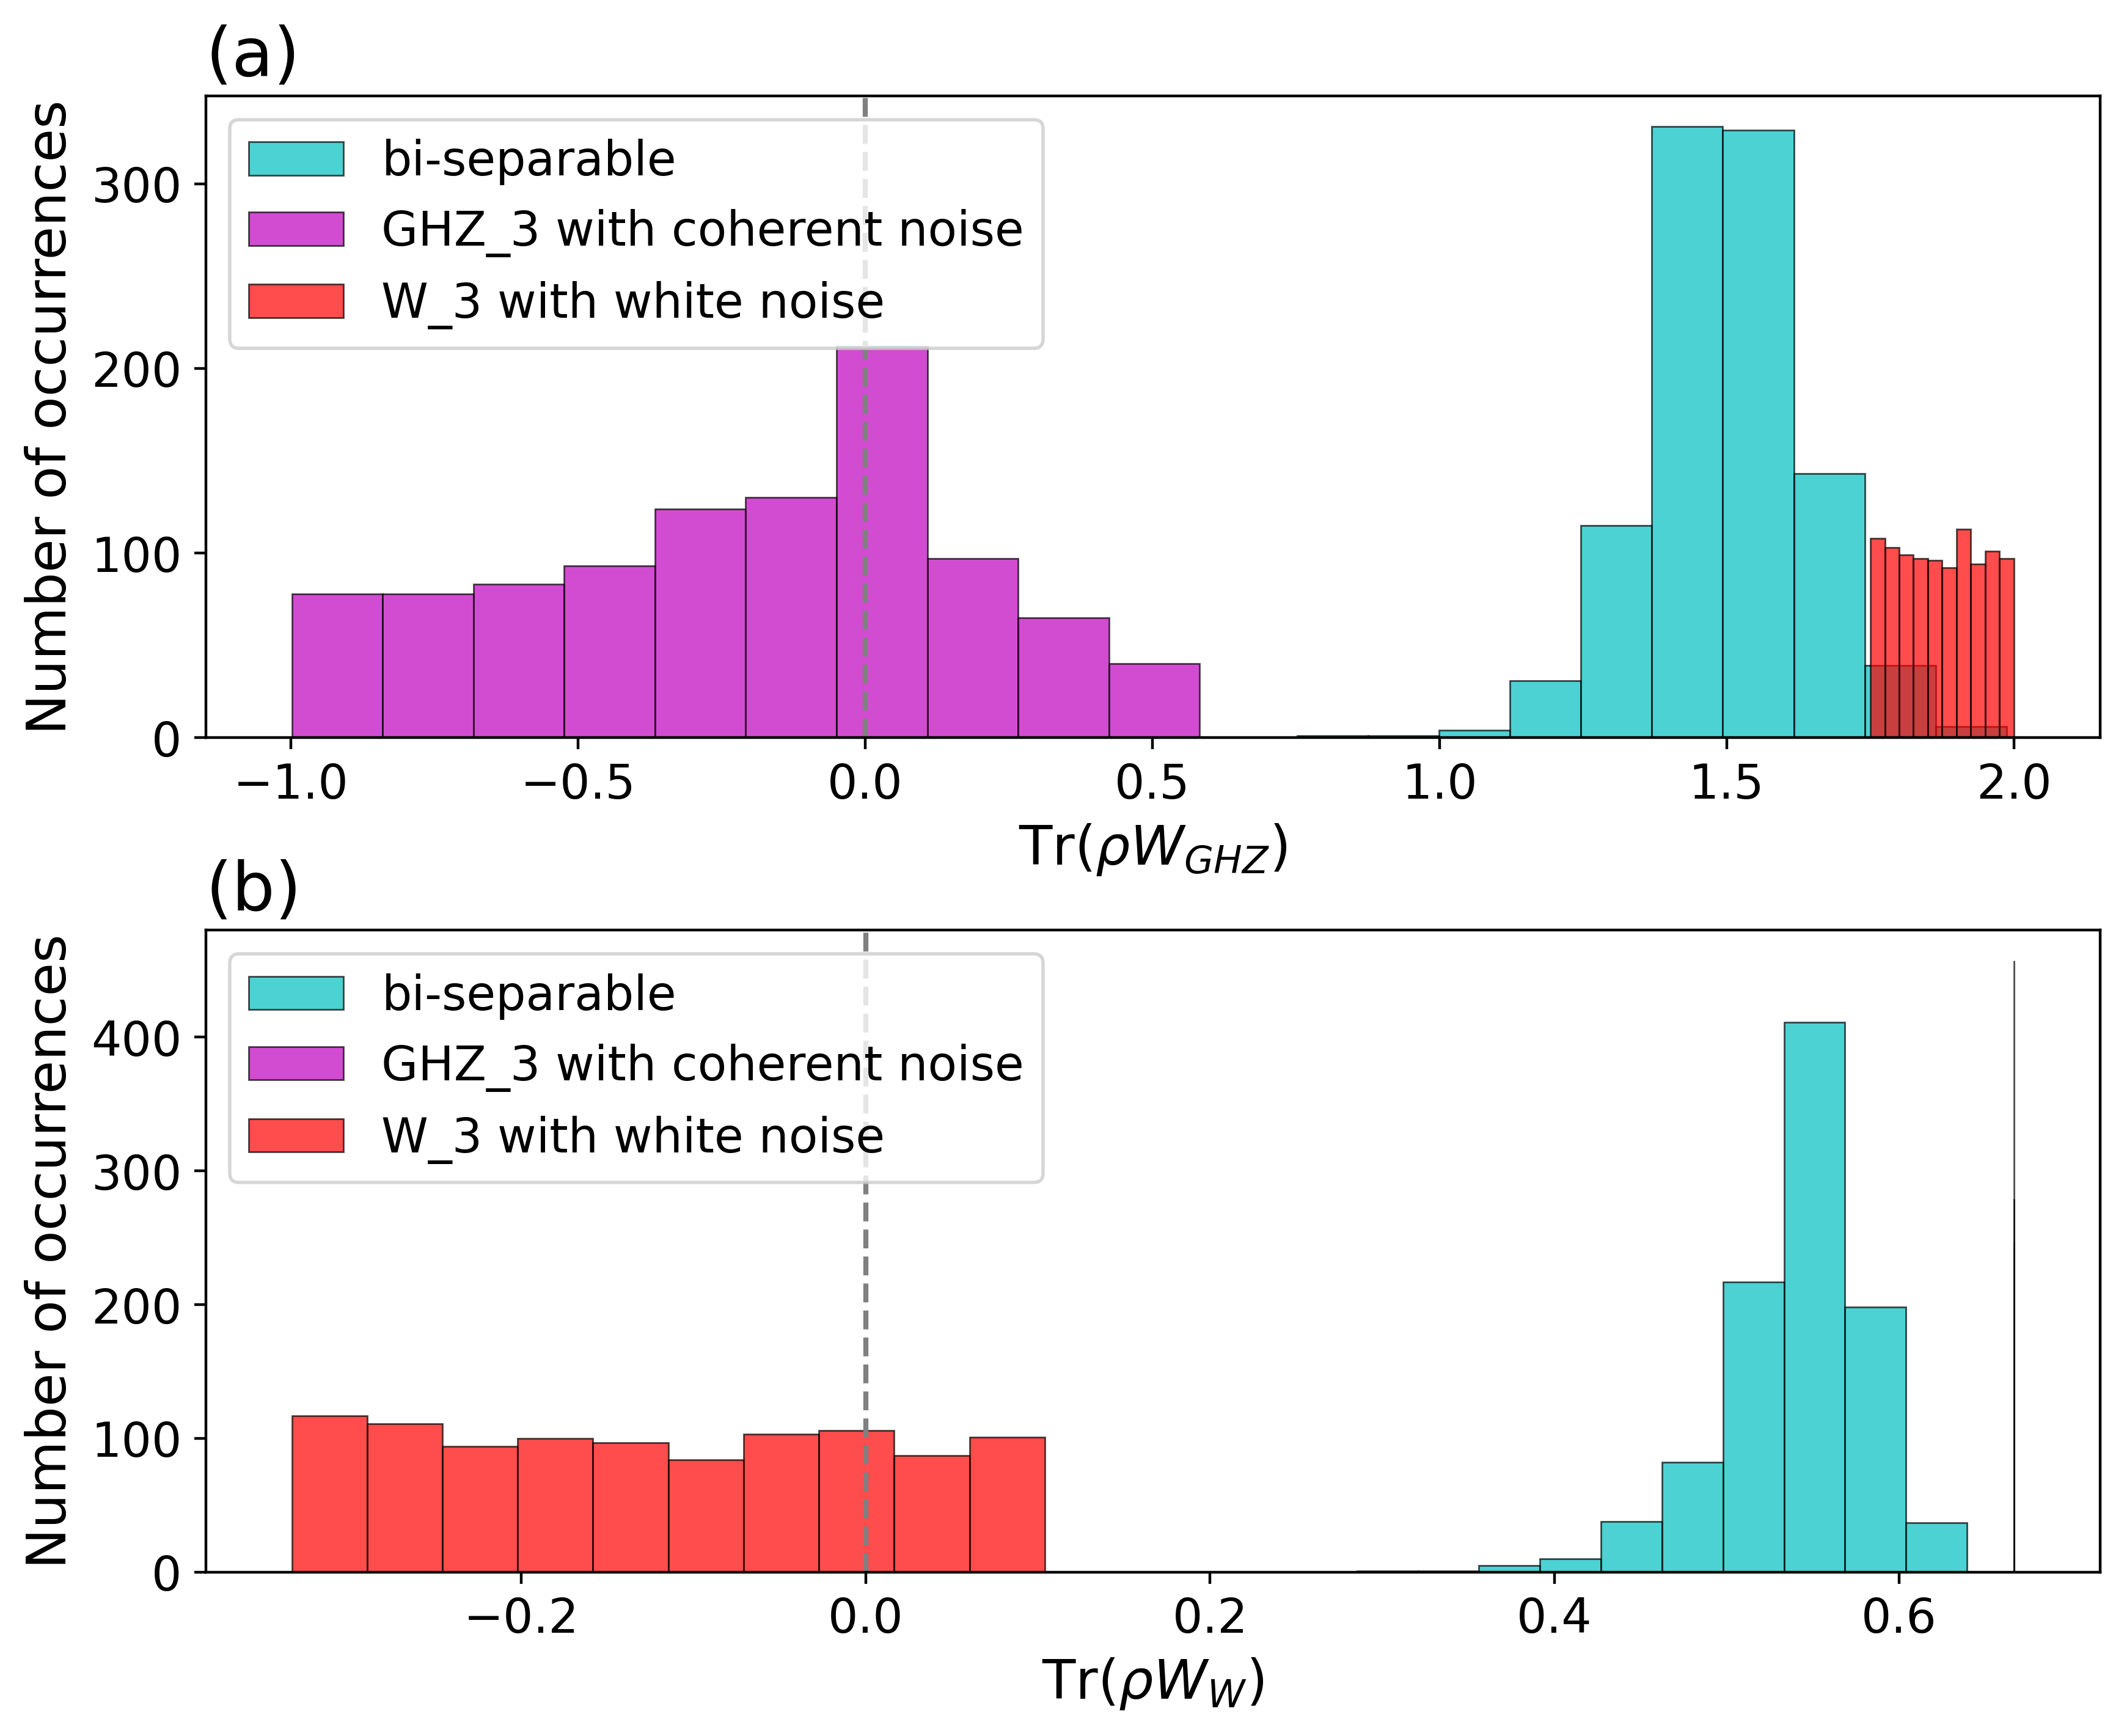
\includegraphics[width=1.0\columnwidth]{./Code/fidelity_witness_compare_2_long.png}%
	}\hfill
	\subfloat{%
	% \subfloat[\label{subfig:b}]{%
		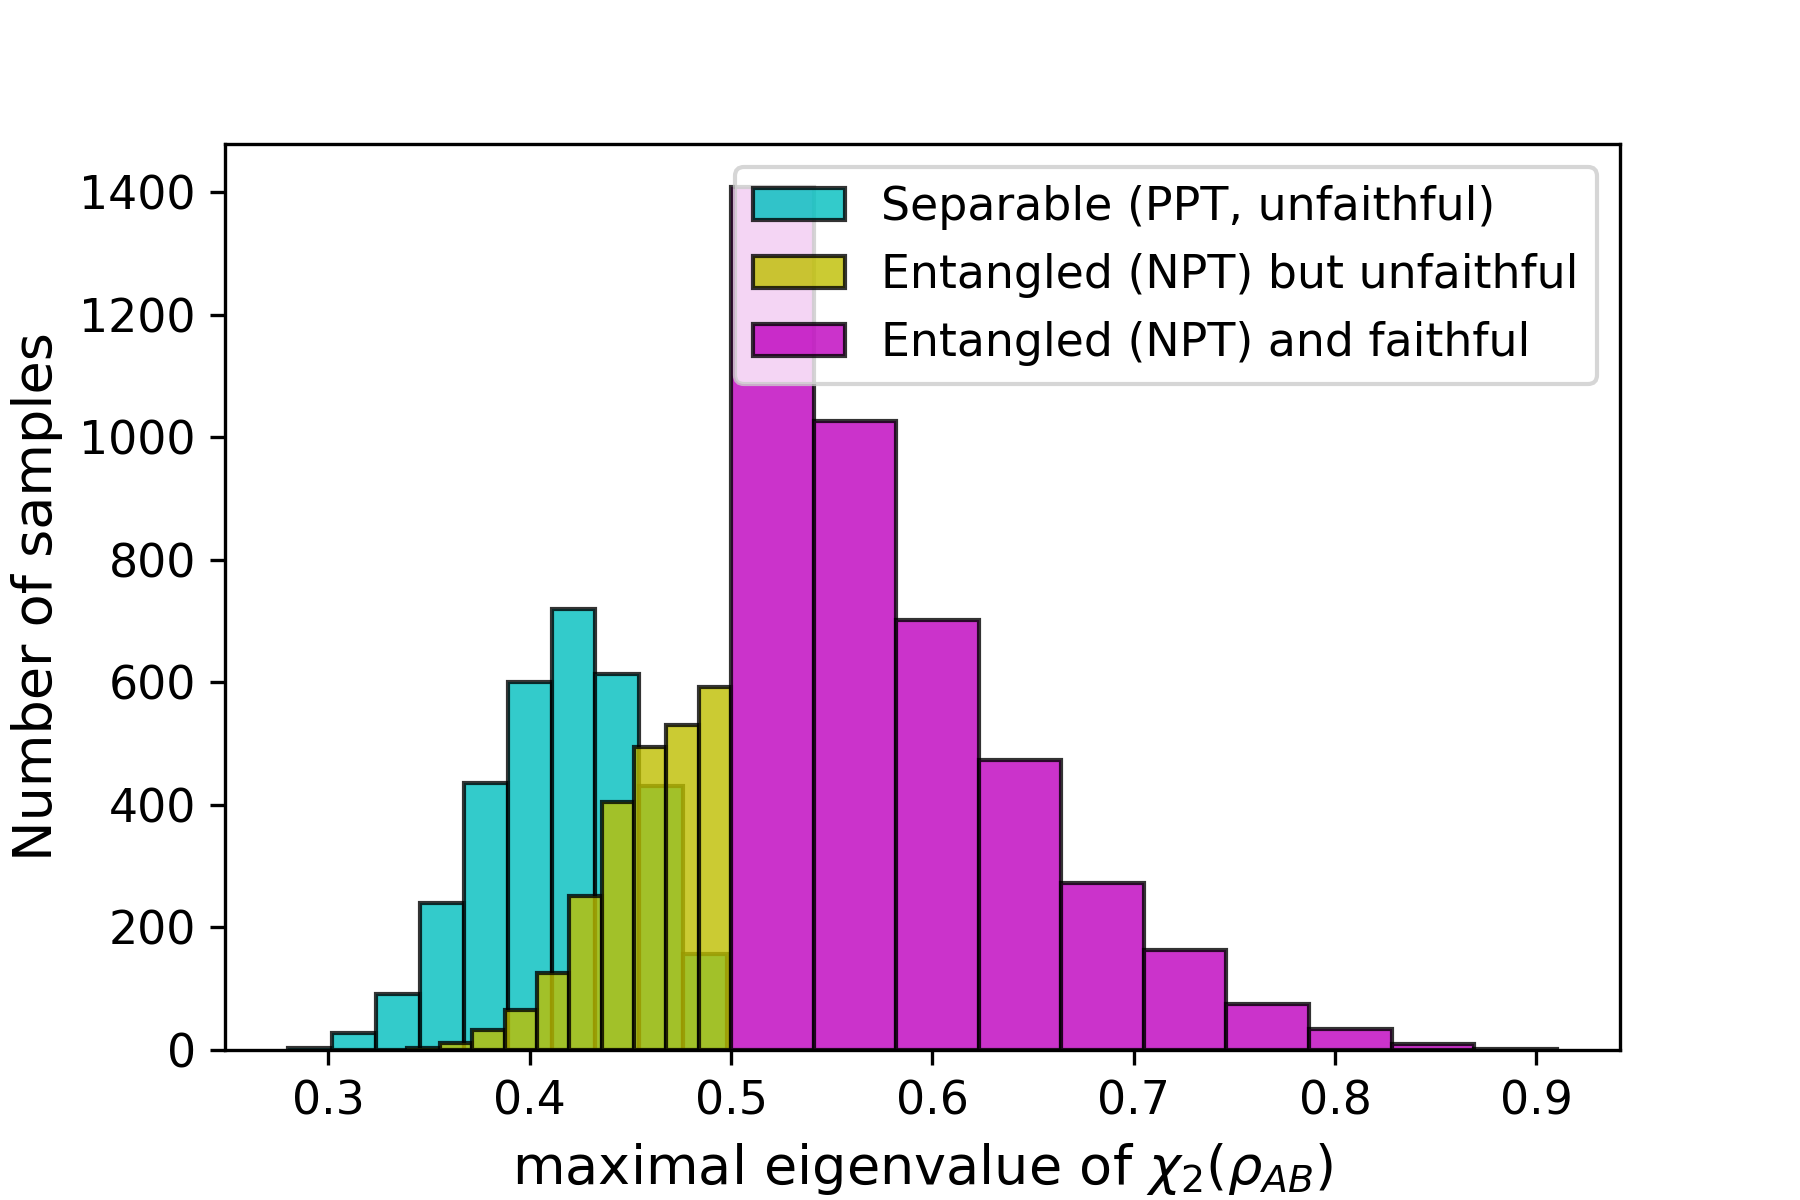
\includegraphics[width=0.9\columnwidth]{./Code/faithfulness_2_qubit.png}%
	}
		% \begin{subfigure}{0.49\textwidth}
		% \centering
		% 	% \includegraphics[width=.9\linewidth]{.pdf}
		% 	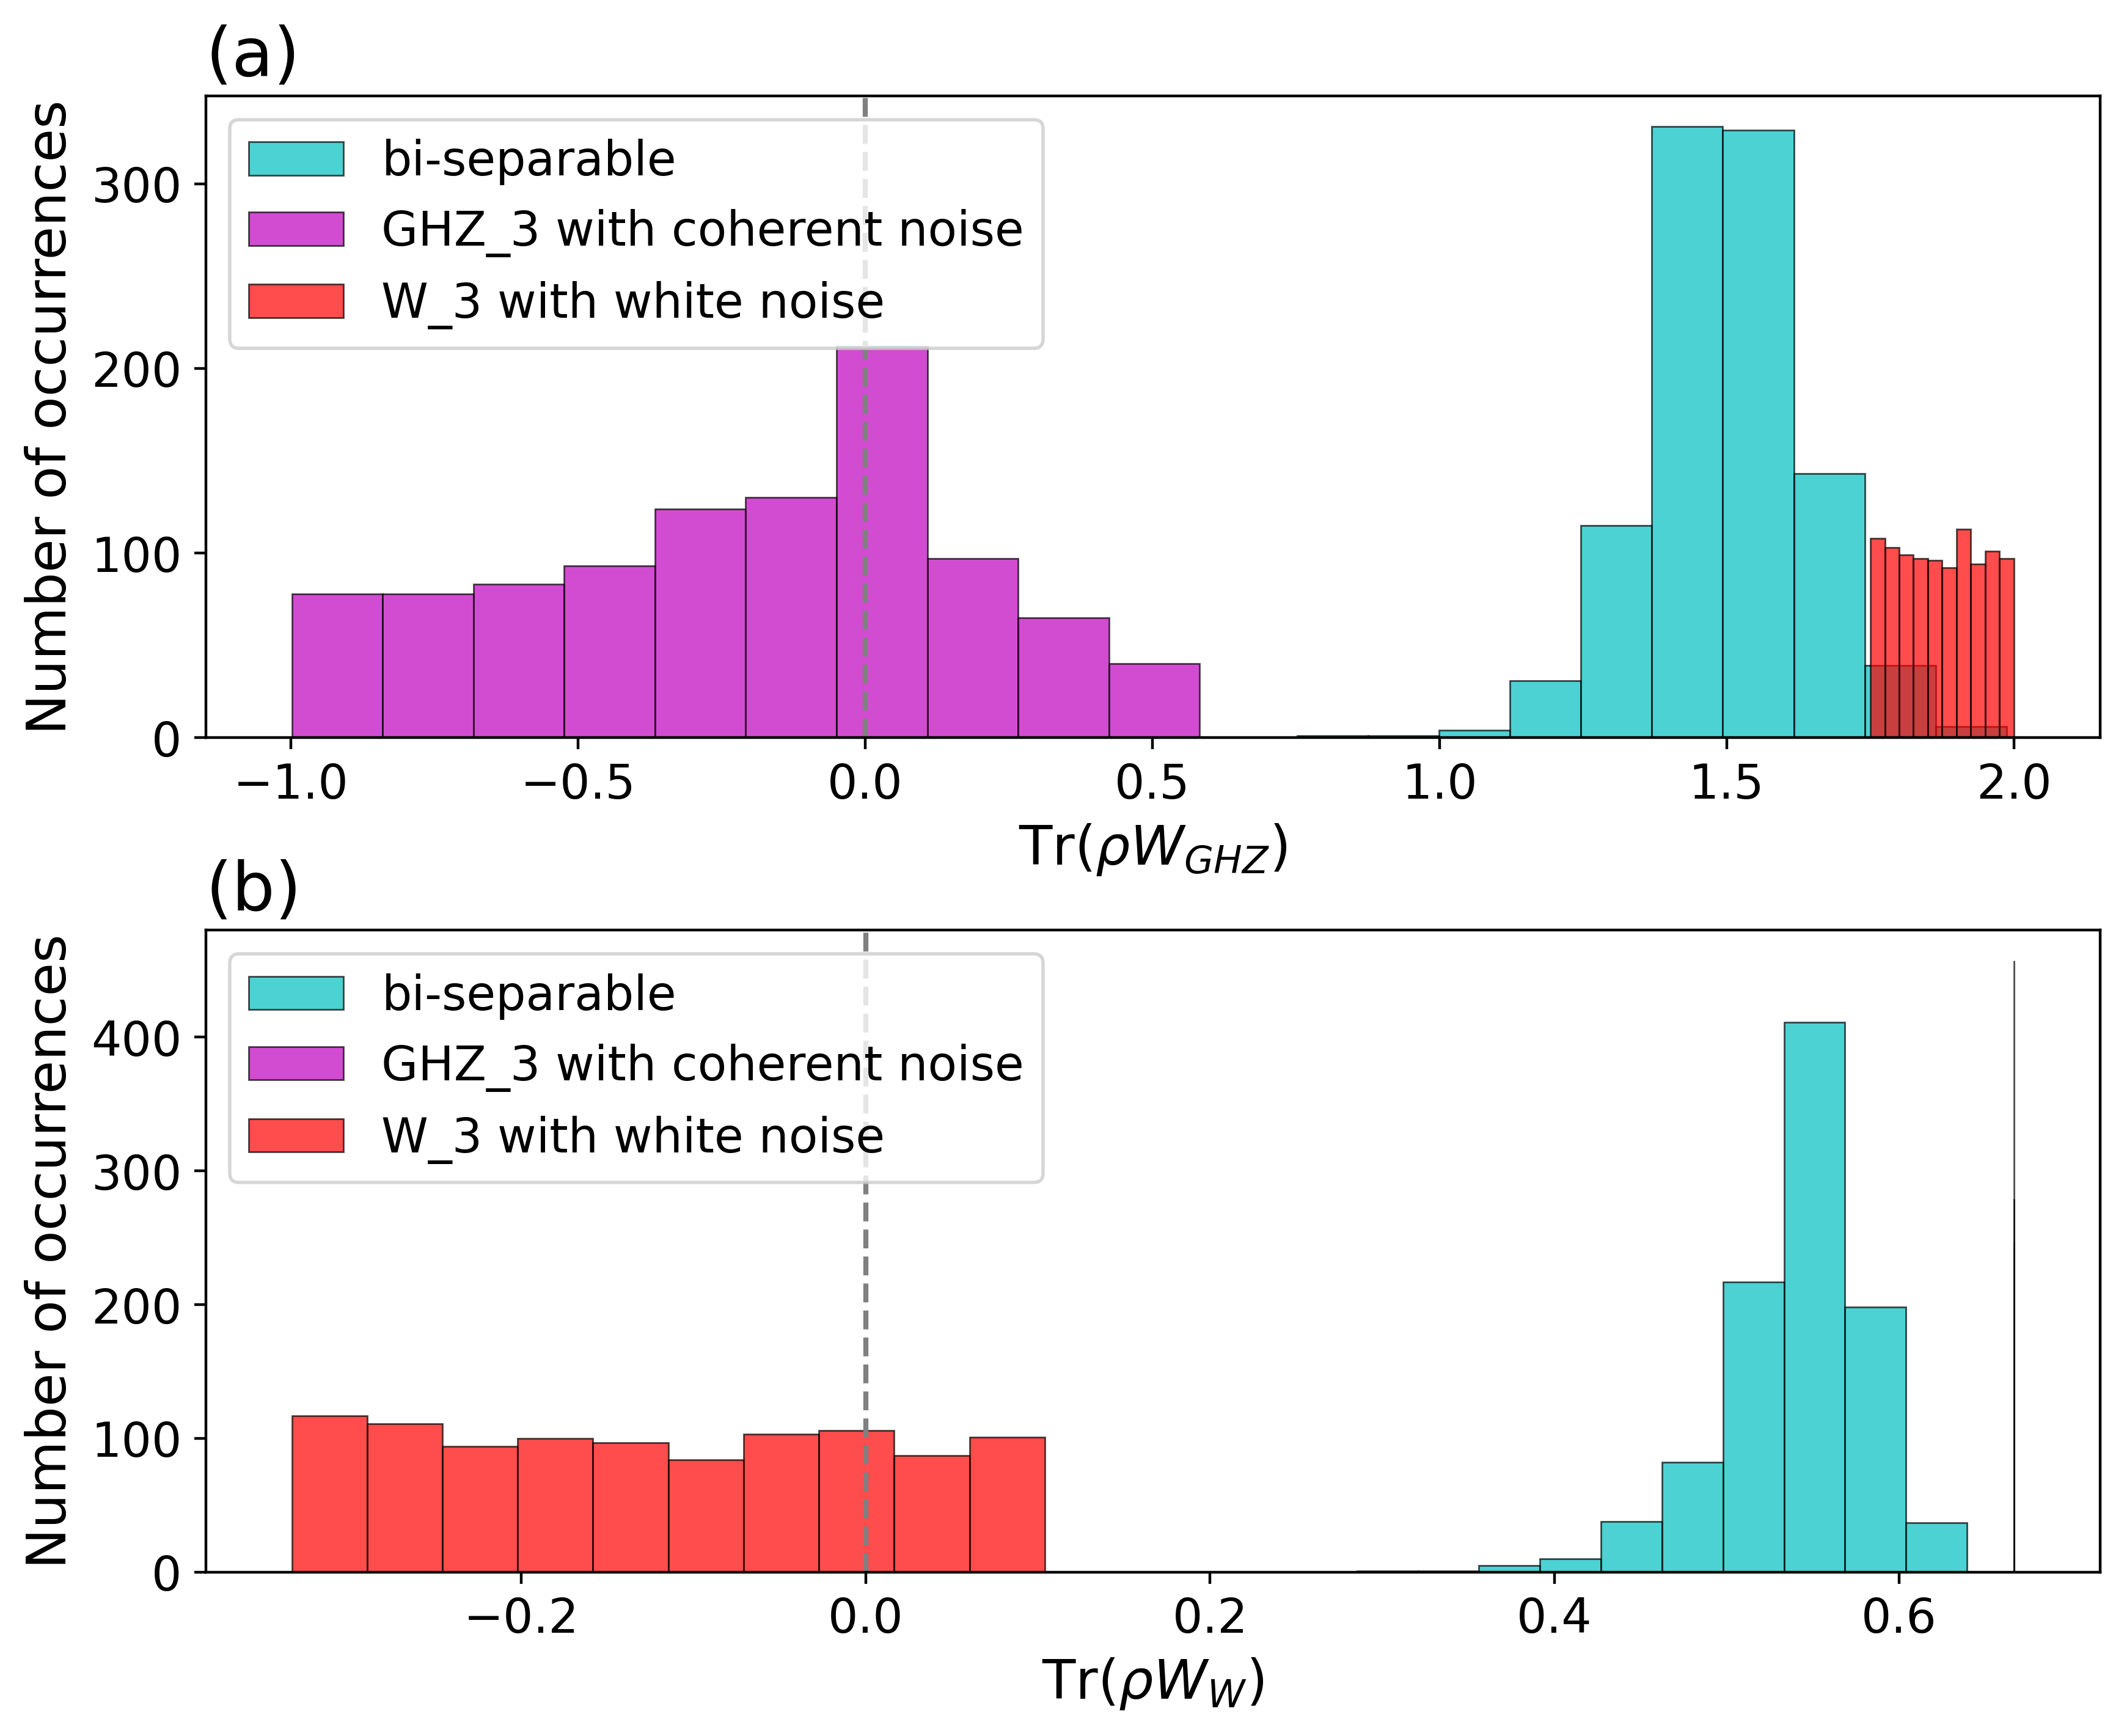
\includegraphics[width=.9\linewidth]{./Code/fidelity_witness_compare_2_long.png}
		% \end{subfigure}
		% \begin{subfigure}{0.45\textwidth}
		% \centering
		% 	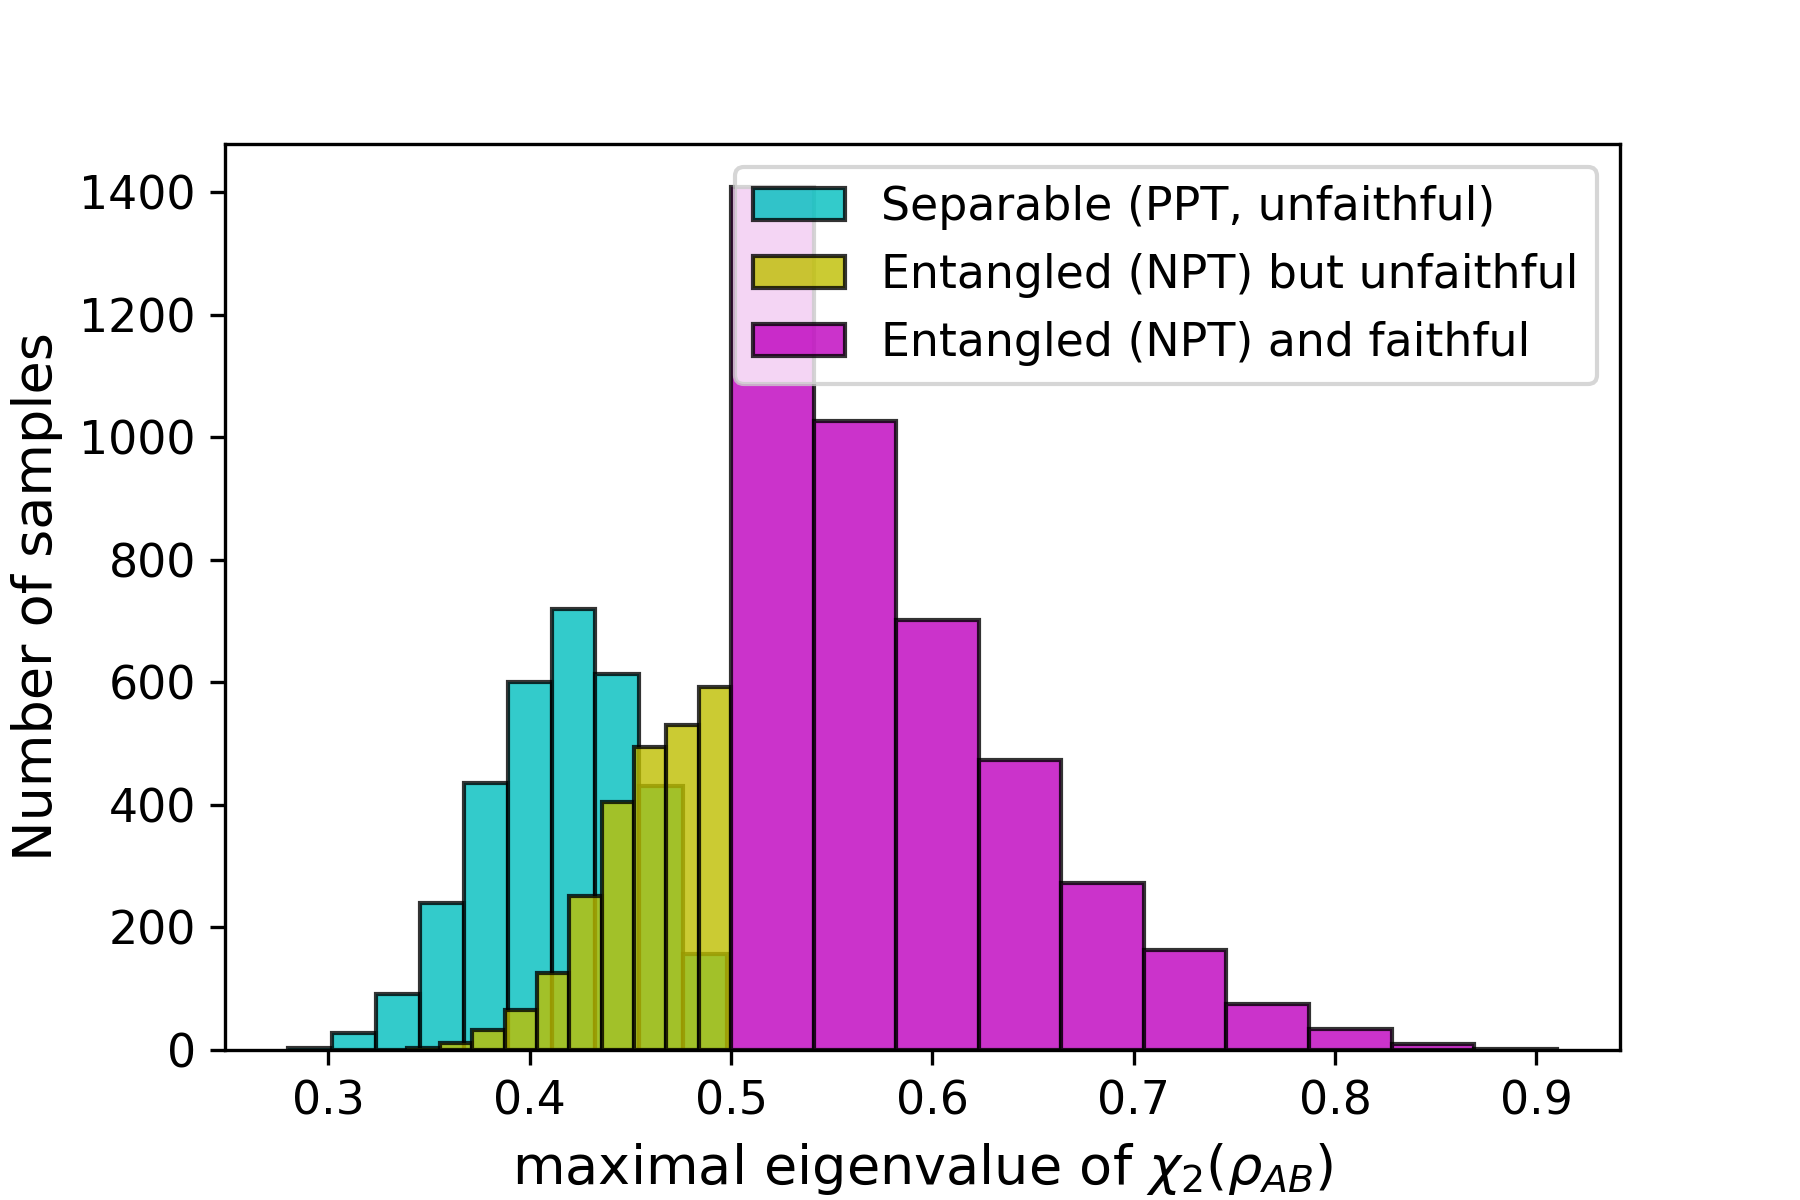
\includegraphics[width=.9\linewidth]{./Code/faithfulness_2_qubit.png}
		% \end{subfigure}
	\caption{Examples of the entanglement states cannot be detected by conventional fidelity witnesses. (a) GHZ states with coherent noise sampled with $\theta=\pi/3$ and $\phi\in[0.5\pi,0.6\pi]$ cannot be detected by the GHZ projector fidelity witness $W_{\ghz}$ (c.f. \cref{eq:entanglement_witness}). Entangled states should be on the left of the dashed vertical line, i.e., have negative expectation value of the witnesses $\Tr(\dm\ew)$. (b) Similarly, W states with large white noise $p_{\noise}\in[8/21,0.5]$ cannot be detected by $W_{\text{w}}$. And we can see W states with white noise has $\Tr(\dm_{\text{W}}\ew_{\ghz})>0$, vice versa. (c) Unfaithfulness of 2-qubit states: $10^4$ randomly sampled 2-qubit states are categorized according to the minimal eigenvalue of partial transpose $\dm_{AB}^{\T_A}$ and the maximal eigenvalue of $\chi_2(\dm_{AB})$.}
	\label{fig:conventional_witness}
	% \caption{(a) compare different methods: Bell inequality, witness, ML ansatz; different white noise limit, unfaithful state; }
\end{figure*}

To formally characterize the cases beyond fidelity witness, Weilenmann et. al \cite{weilenmannEntanglementDetectionMeasuring2020} \cite{huOptimizedDetectionHighDimensional2021} coined the term \emph{unfaithful states} 
which systematically analyze 2-qudit entangled state mixed with white noise that cannot be detected by fidelity witness.
They found that for $d \ge 3$ that almost all states in the Hilbert space are unfaithful. 
% For $d > 5$, the authors find that all states they generated are entangled but at the same time unfaithful, regardless of what metric is used to sample them.
% faithful states are useful for quantum teleportation.
% This shows that fidelity-based entanglement witnesses detect entanglement that is useful for teleportation.
Subsequently, G\"{u}the et. al \cite{guhneGeometryFaithfulEntanglement2021} \cite{riccardiExploringRelationshipFaithfulness2021} gave a formal definition: 
% the faithfulness of a twoqubit state, allowing for a physical interpretation of unfaithful two-qubit states as exactly those entangled states that are not useful for teleportation.
% \begin{definition}[unfaithful state]\label{def:unfaithful_state}
	% informally, unfaithful state are entangled states but cannot be detected by fidelity witness.
	a 2-qudit state $\dm_{AB}$ is faithful if and only if there are local unitary transformations $\U_A$ and $\U_B$ such that
	$\expval{\U_A\otimes\U_B \dm_{AB} \U_A^\dagger \otimes\U_B^\dagger}{\phi^+}> \frac{1}{d}$.
	% \begin{equation}
	% 	\expval{\U_A\otimes\U_B \dm_{AB} \U_A^\dagger \otimes\U_B^\dagger}{\phi^+}
	% 	> \frac{1}{d}.
	% \end{equation}
% \end{definition}
Consequently, they found a necessary and sufficient condition for 2-qubit unfaithfulness: 
% determined by the spectrum of
a 2-qubit state $\dm_{AB}$ is faithful if and only if the maximal eigenvalue of
\begin{equation}
	\mathcal{X}_2( \dm_{AB})=\rho_{AB}-\frac{1}{2}(\dm_{A}\otimes I + I \otimes \dm_{B})+\frac{1}{2} I \otimes I
	\label{eq:unfaithful_2qubit}
\end{equation}
is larger than 1/2.
We can see in (c) of \cref{fig:conventional_witness}, even for 2-qubit states, nonnegligible portion of randomly sampled states are unfaithful but still entangled (NPT).
% \begin{figure}[!ht]
% 	\centering
% 	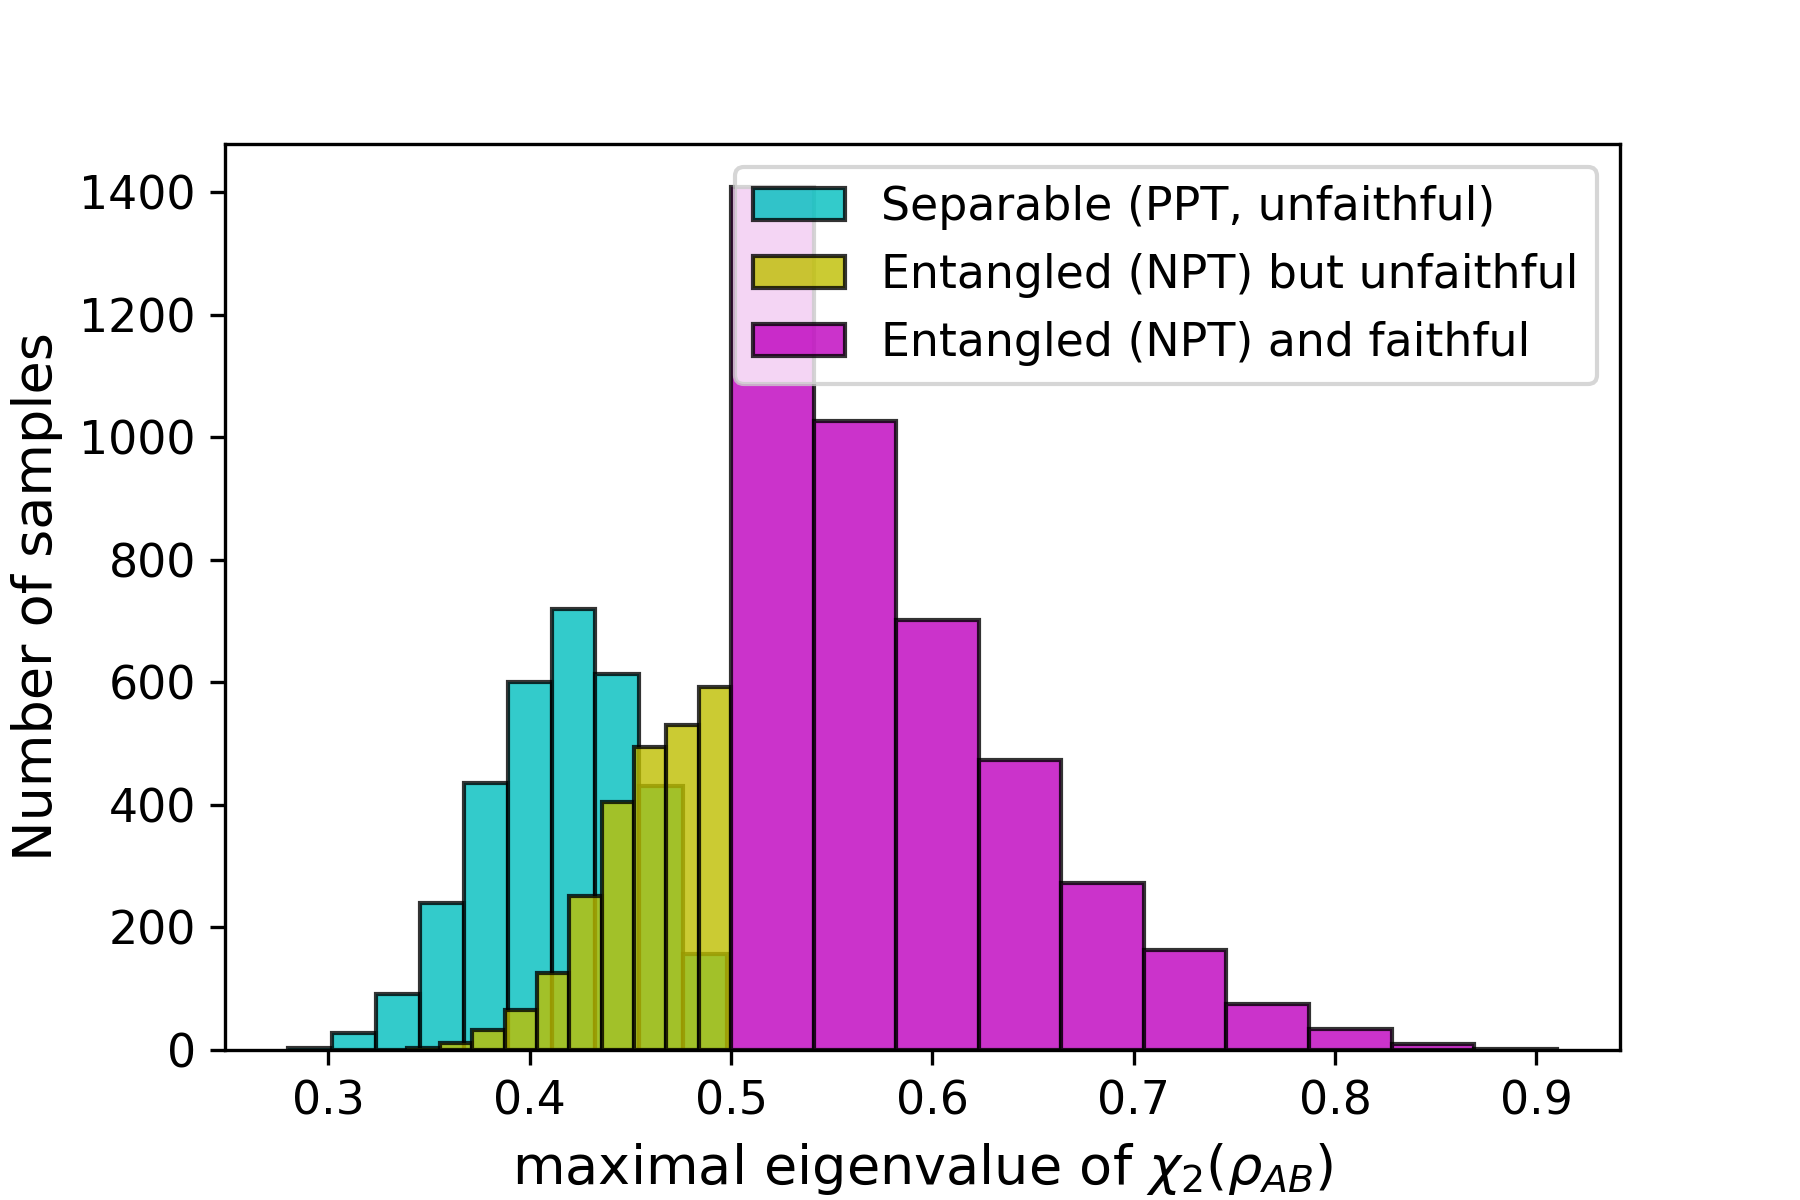
\includegraphics[width=.9\linewidth]{./Code/faithfulness_2_qubit.png}
% 	% \caption{PPT criterion (2-qubit random density matrix)}
% 	\caption{Unfaithfulness of 2-qubit states: $10^4$ randomly sampled 2-qubit states are categorized according to the minimal eigenvalue of partial transpose $\dm_{AB}^{\T_A}$ and the maximal eigenvalue of $\chi_2(\dm_{AB})$.}
% 	\label{fig:unfaithfulness}
% \end{figure}

Although there are variants of witness, such as nonlinear witness \cite{guhneNonlinearEntanglementWitnesses2006} and post-processing \cite{zhanDetectingEntanglementUnfaithful2021}, designed to remedy the shortcomings of conventional fidelity witness respectively, 
% \cite{huOptimizedDetectionHighDimensional2021}
it would be meaningful in practice to find a generic method to construct witnesses (classifiers) for \nameref{prm:entanglement_detection}.
% Moreover, they can only be applied to bipartite systems, which means they cannot be generalized to detect genuine entanglement in multipartite states.
Machine learning techniques suit the needs well because supervised learning can be regarded as a powerful nonlinear post-processing tool.


\subsection{Training a generic witness via kernel SVM}
% \section{End-to-end entanglement detection protocol}\label{sec:protocol}
% \section{Classical-quantum hybrid, end-to-end detection protocol}
% \section{Classical, data-powered, and quantum algorithms}
% In this paper, we focus on the entanglement structure dectection for graph states.
One basic task in classical machine learning (ML) is binary classification,
such as cat/dog images classification. 
In this case, the input to a ML algorithm is a (training) dataset $\qty{(\vbx^{(i)},y^{(i)})}_{i=1}^m$ consists of $m$ data points, 
where each data point is a pair of feature vector $\vbx\in \realnumber^d$ of $d$ features and its label $y\in\qty{-1,1}$.
For example, the feature $\vbx$ of an image is a flatten vector of all pixel values and the label $y=-1$ for \textsc{cat} images ($1$ for \textsc{dog}).
It is clear that \nameref{prm:separability} or \nameref{prm:entanglement_detection} problem are exactly such binary classification problems where each quantum state has a binary label, such as either `\entangled' or `\separable'.
The features $\vbx$ of a quantum state $\dm$ can be the entries of its density matrix, or more realistically, the expectation values of selected observables.
% formally in \cref{sec:svm}
% The quantum extension of this problem (classficiation/pattern recognition) is to replace the data points with density matrices of quantum states . 
% Specifically, a quantum state classifier outputs a label associated with the state, such as, $\entangled$ or `bi-separable'.

With the surge of research on machine learning, ML algorithms have been proposed for classification tasks related to entanglement.
Lu et. al \cite{luSeparabilityEntanglementClassifierMachine2018} 
trained a (universal) \nameref{prm:separability} classifier by classical neural network
where features of $\vbx$ are the entries of density matrices.
% where input dataset are (randomly sampled) density matrices  with labels?.
For the similar purpose, Ma and Yung \cite{maTransformingBellInequalities2018} generalized Bell inequalities to a Bell-like ansatz $\ew_{\ml}:=\vbw_{\ml}\cdot\vb{\pob}_{\bellineq}$ where the optimal weights $\vbw_{\ml}$ are obtained via optimizing a neural network.
% an ansatz for \nameref{def:entanglement_witness} 
% Different Bell inequalities can be regarded as entanglement witness for different types of entanglement in a multi-party entangled state.
% (graph state entanglement)
And they found the tomographic ansatz
\begin{equation}
	\Tr(\dm\ew_{\ml}) \equiv\expval{\ew_{\ml}} := 
	\vbw_{\ml} \cdot \expval{\vb{\pob}_{\sigma}}, 
	\; \forall \sigma \in  \qty{I,X,Y,Z}^n
	% \sum_{k_1,k_2,\dots,k_n}  w_{k_1,k_2,\dots,k_n} \bigotimes_i^n \hat{\sigma}^{(k_i)}
	% ,\quad \hat{\sigma} \in \qty{\sx,\sy,\sz,\identity_{2\times 2}}
	% \sum_{\vb{p}\in \qty{I,X,Y,Z}^n} w_{\vb{p}}  \bigotimes_i^n \vb{p}_i
	% \hat{\sigma}^{(\vb{p}_i)}
	\label{eq:tomographic_ansatz}
\end{equation}
where the feature $\vbx_{\dm,\bmsigma}:=\expval{\vb{\pob}_{\sigma}}$ is the vector of expectations of all $4^n$ Pauli observables
\footnote{
	Denote $\pob_{\sigma}\in \qty{I,X,Y,Z}^{\otimes n}$ for a Pauli observable.
	Denote $\vbx_{\dm,\bmsigma}:=(\Tr(\dm\pob_{\sigma_1}),\dots,\Tr(\dm\pob_{\sigma_M}))$ for expectations of $M$ Pauli observables $\bmsigma\subseteq \qty{I,X,Y,Z}^n$ with respect to the state $\dm$. 
},
% c.f. \nameref{prm:full_tomography} 
not only has better performance than the Bell-like ansatz, 
also required \cite{luTomographyNecessaryUniversal2016} for training a universal \nameref{prm:separability} classifier.
It is worth noting that training such a universal classifier for high-dimensional systems is a difficult optimization problem if the gap between two state sets is small (weak promise).

\begin{figure*}[!ht]
	\centering
		\centering
		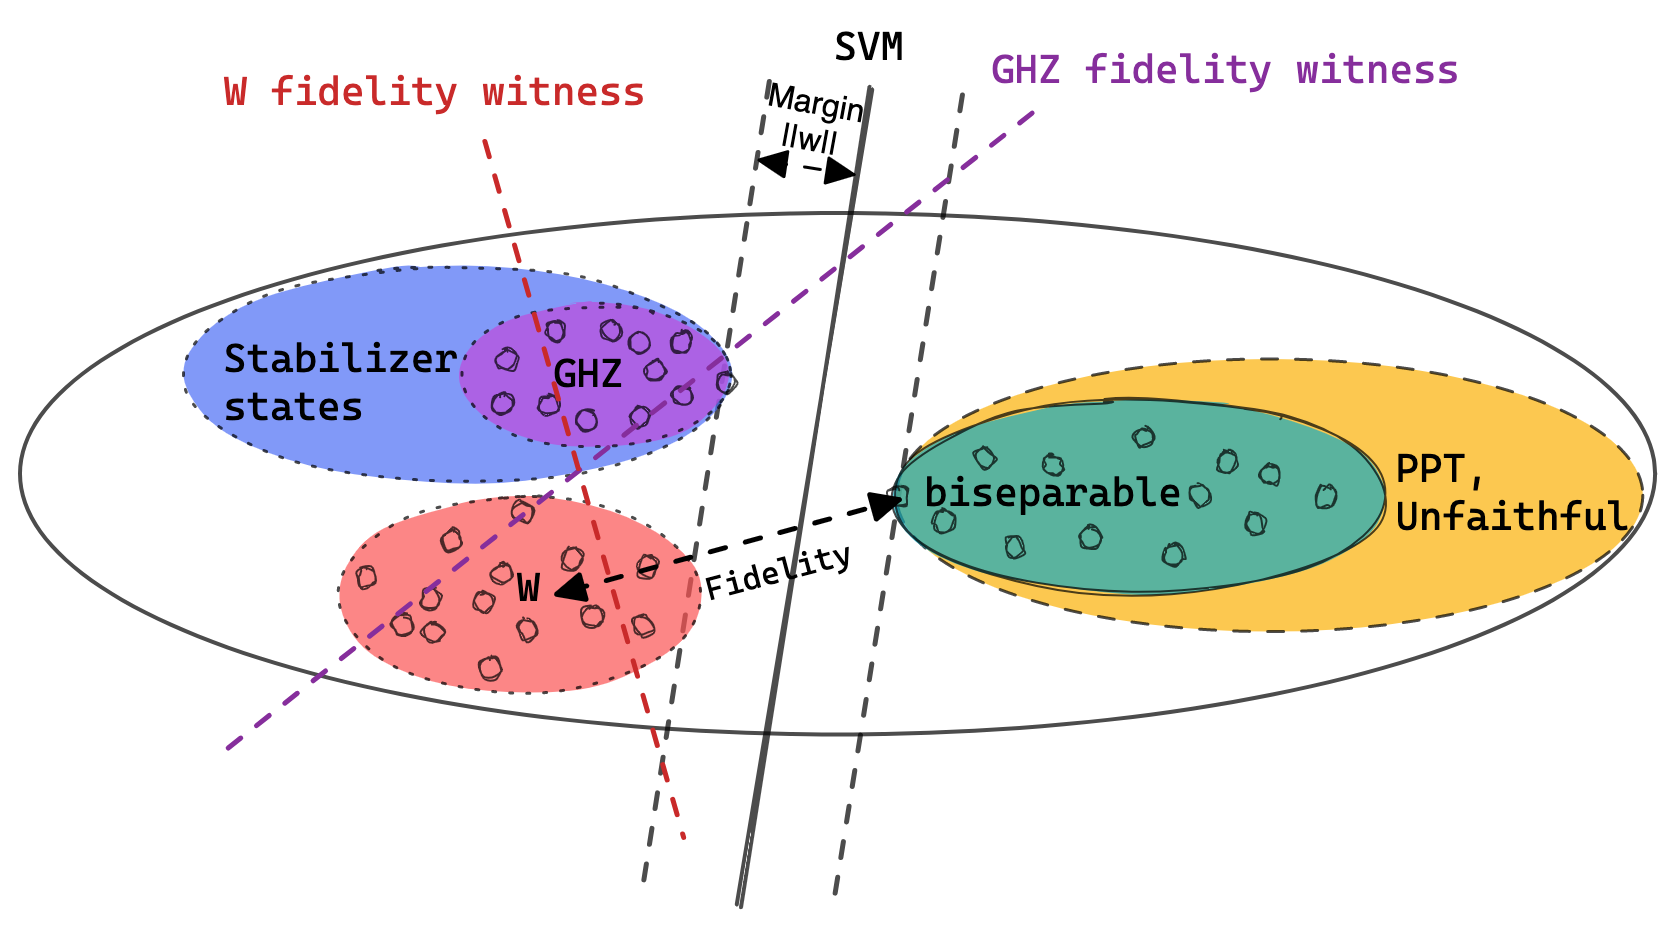
\includegraphics[width=.6\linewidth]{schematic.png}
	% 	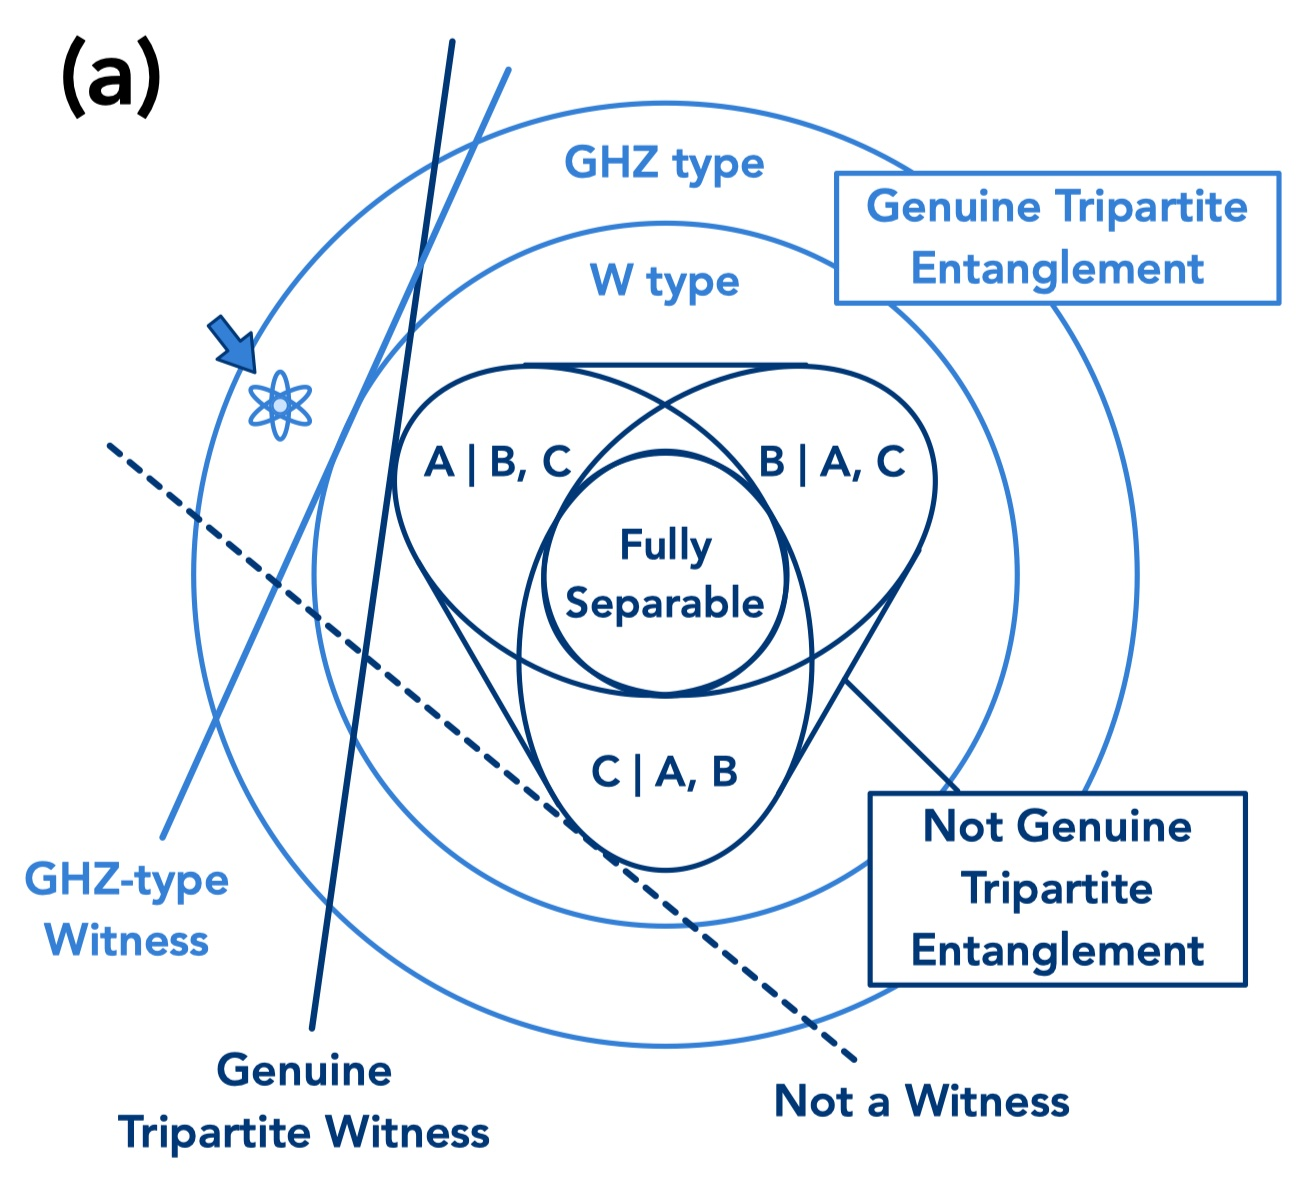
\includegraphics[width=.9\linewidth]{gme.jpg}
	% . 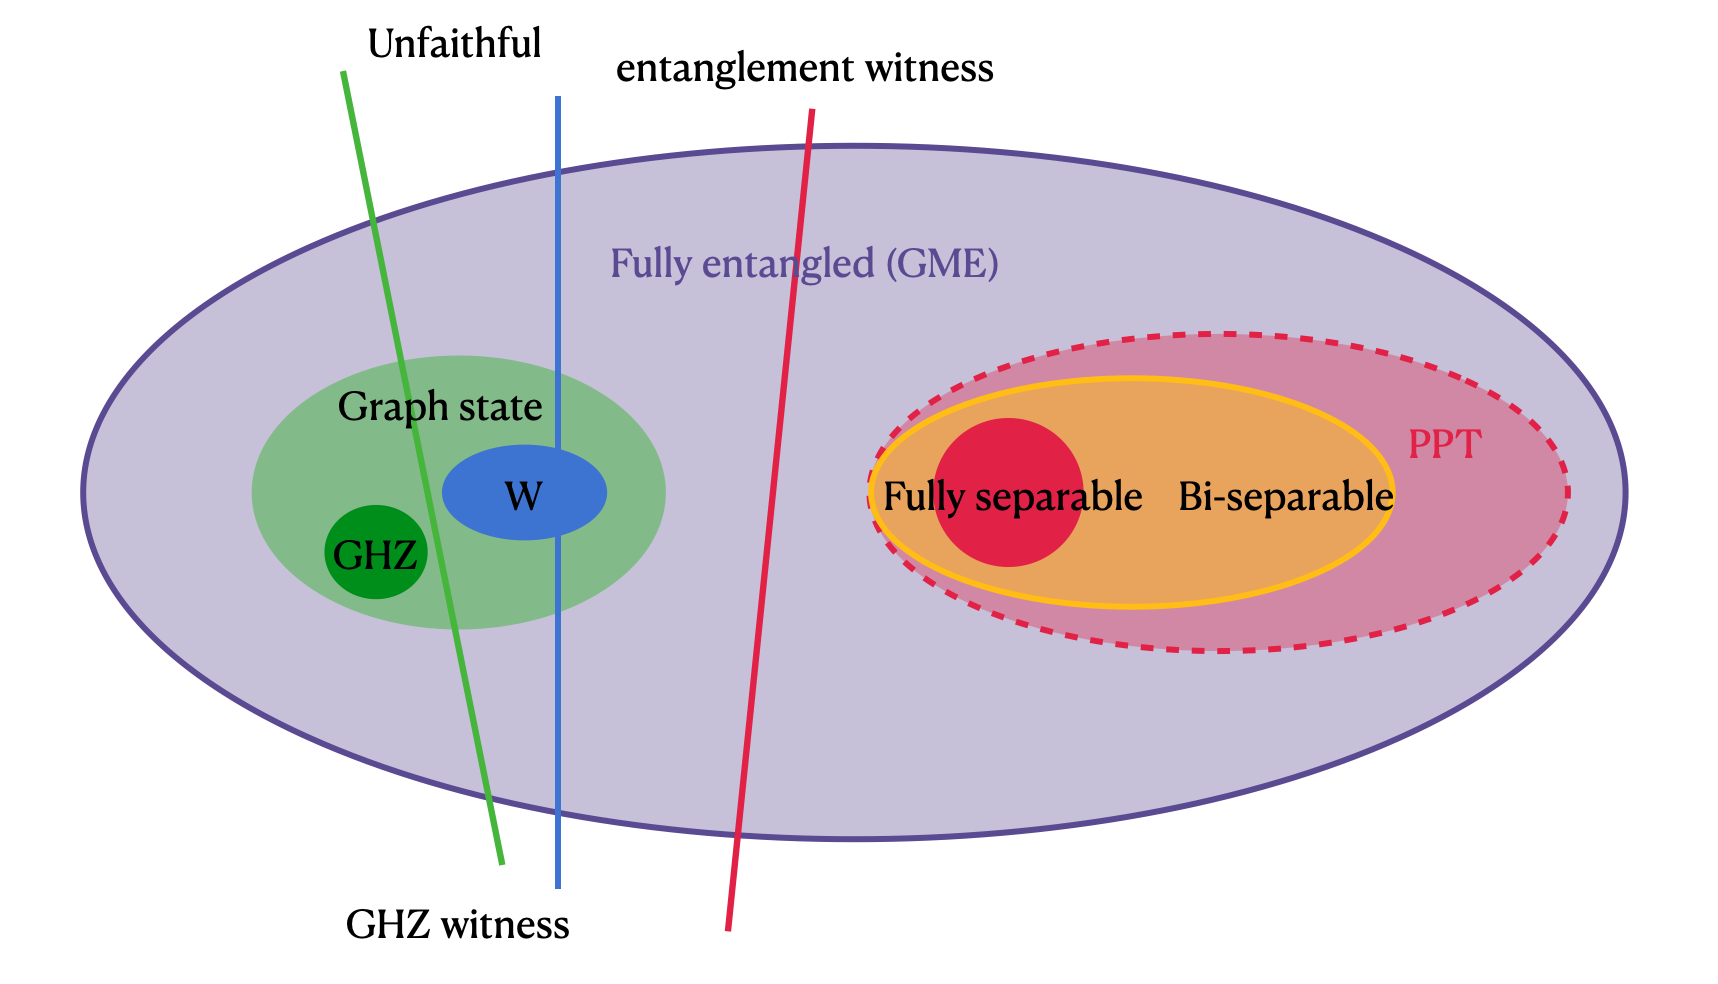
\includegraphics[width=.7\linewidth]{witness.png}
	% 	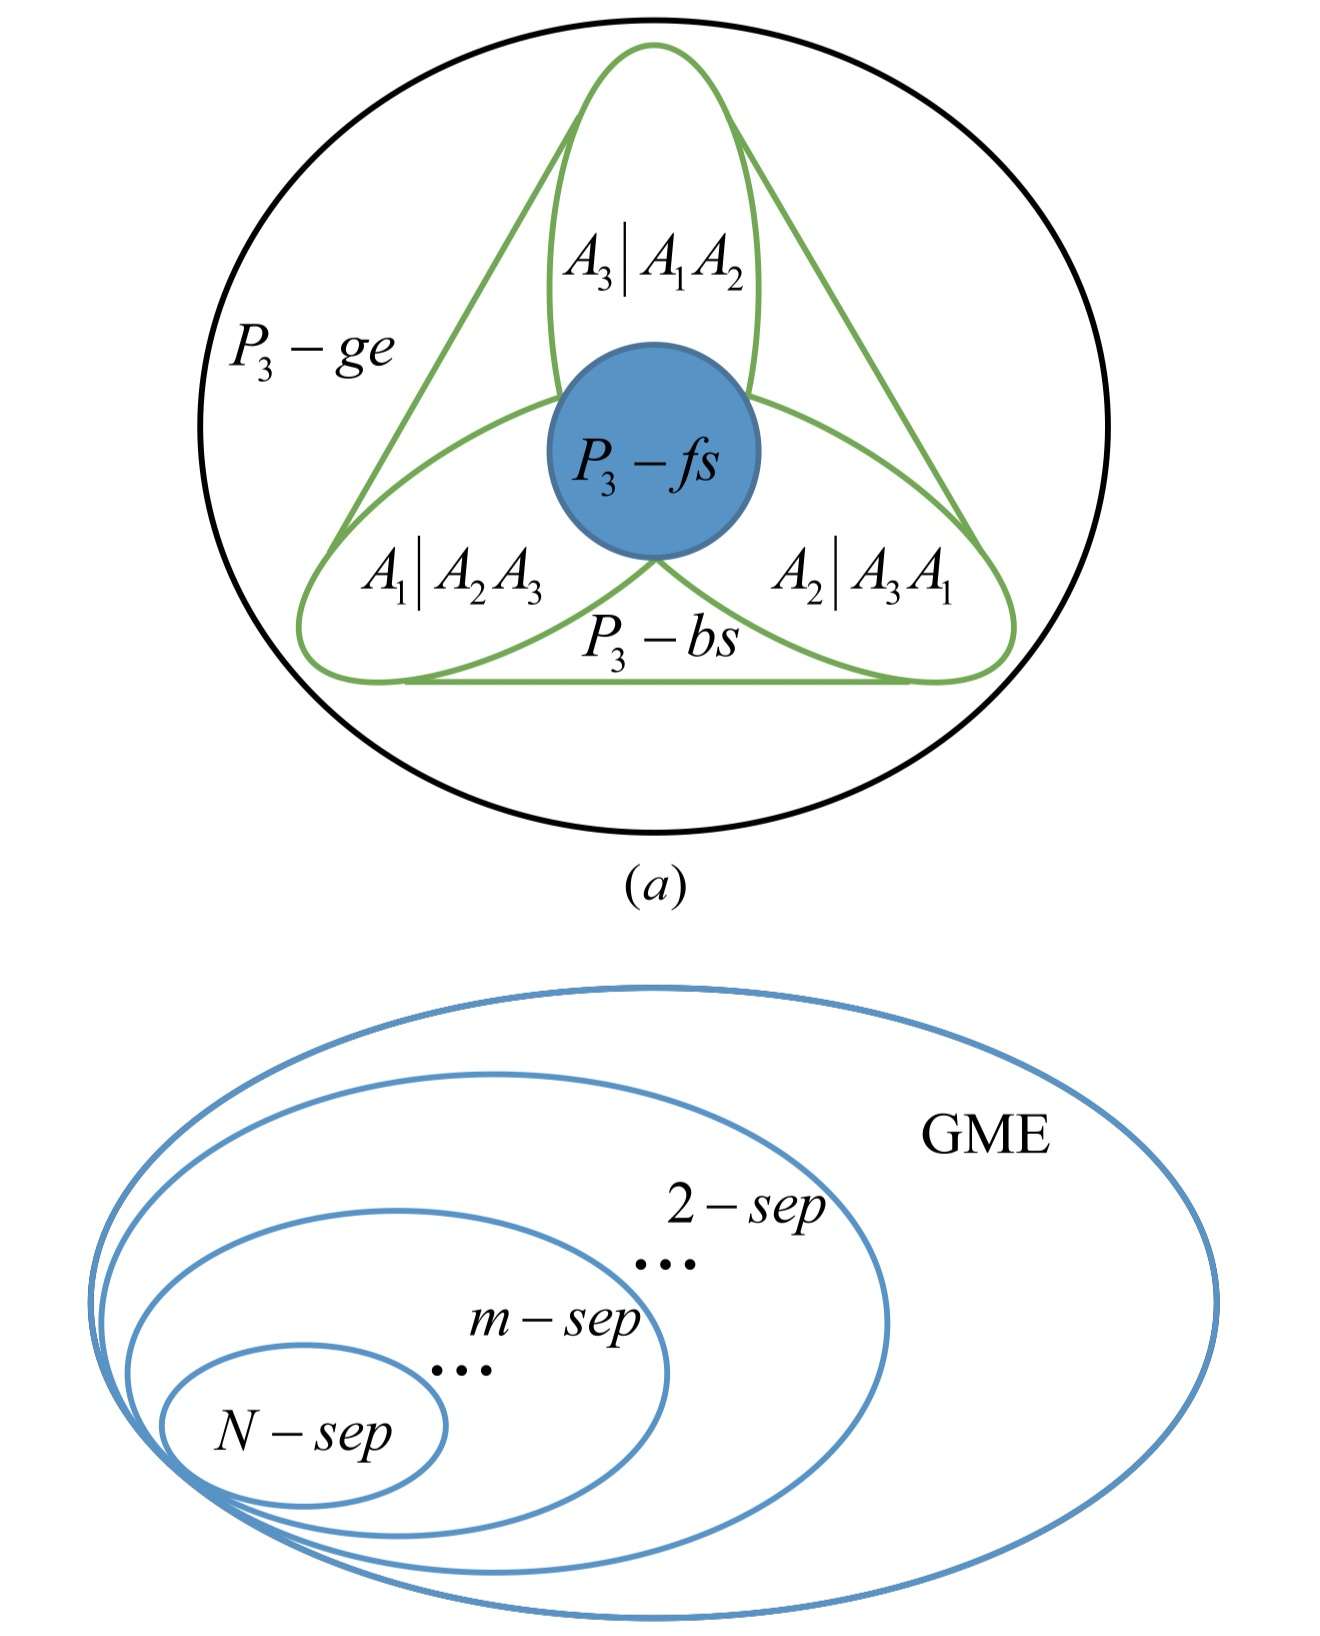
\includegraphics[width=.8\linewidth]{sep.jpg}
	% 	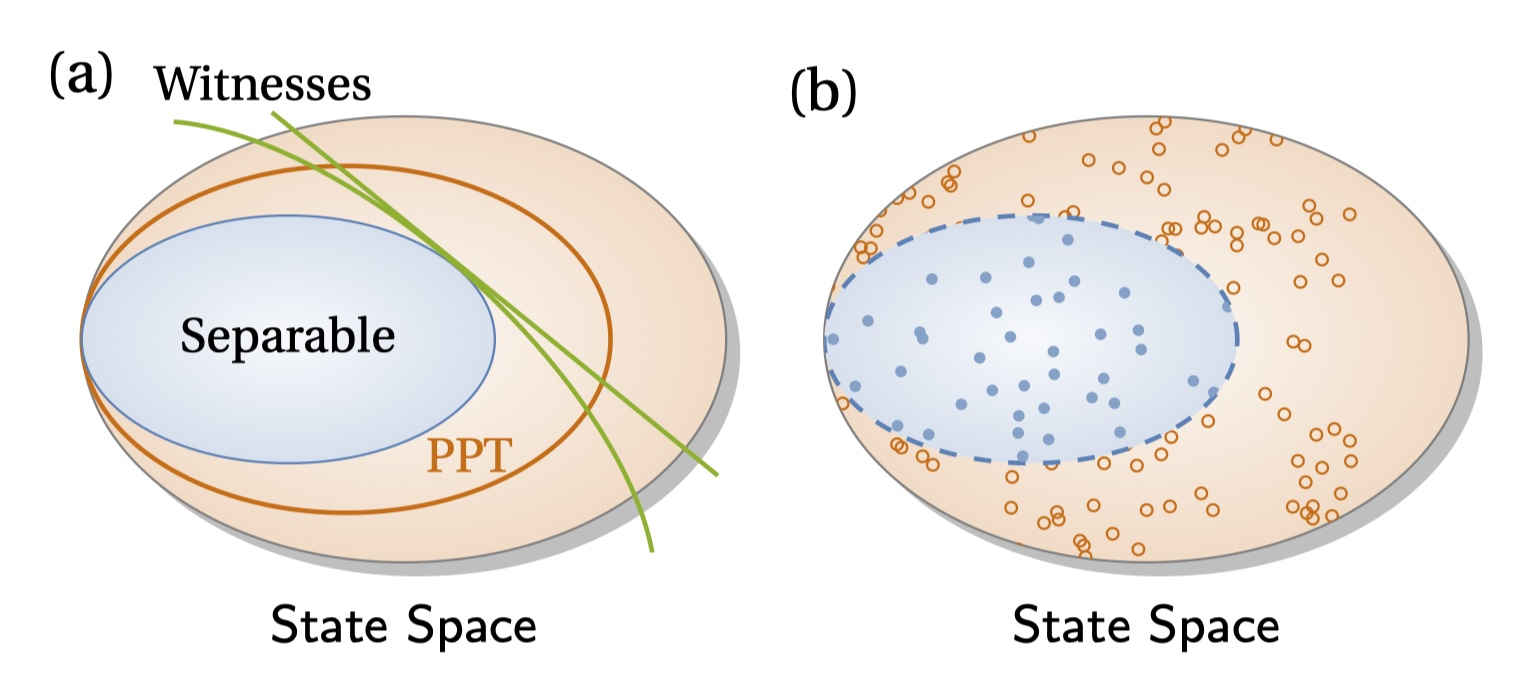
\includegraphics[width=.9\linewidth]{ppt.jpg}
	\caption{Schematic diagram for different entanglement detection methods: the colored ellipses without black boundary indicate the vicinity (white noise) of certain entangled state such as GHZ, W states. Conventional fidelity witnesses for different states are depicted by colored dash lines (hyperplanes in feature space). Entangled state with large white noise or coherent noise (local rotation depicted by a curve) cannot be detected by conventional fideilty witnesses. SVM without kernel is a hyperplane separating two sets of colored dots (synthetic dataset). The data points on the boundaries (dashed black lines) are called support vectors. The distance between the SVM hyperplane and boundary is the margin to be minimized via optimization. The PPT criterion is a nonlinear but one-side classifier without prior knowledge.}
	\label{fig:entangle}
\end{figure*}

% \subsection{Training a generic witness via SVM}
In our paper, we focus on the \nameref{prm:entanglement_detection} problem with training data.
In other words, we derive the entanglement witness (classifier) for certain target states with desired entannglement structure by fitting a synthetic dataset.
\begin{problem}[learning an entanglement witness]\label{prm:learn_witness}
	% It aims to learn a witness for \nameref{prm:entanglement_detection} of the target entangled state $\ket{\psi_{\target}}$ from a synthetic dataset
	% \hfill
	\;
	\begin{itemize}
		\item \textbf{Input}: a dataset $\qty{\qty(\dm^{(i)},y^{(i)})}$ consist of randomly sampled entangled states $\dm$ around $\ket{\psi_{\target}}$ with label $y=-1$ and randomly sampled separable states with label $1$.
		\item \textbf{Output}: a learned classifier $f(\vbx_{\dm,\tilde{\bmsigma}})$ with high training accuracy where $\tilde{\bmsigma}$ is a subset of all Pauli observables and $\vbx_{\dm,\tilde{\bmsigma}}$ is a vector of corresponding expectation values.
		% (minimal) 
	\end{itemize}
\end{problem}

% \begin{problem}[detect graph state entanglement structure?]
% 	problem with/without training data
% 	\begin{itemize}
% 		\item \textbf{Input}: a graph $\graph$ encoding in a graph state $\ket{\graph}$;
% 		adjacency matrix $A$?
% 		\item \textbf{Output}: entanglement structure: \textsf{\nameref{def:gme}}??
% 	\end{itemize}
% % with training data: 
% \end{problem}
% \begin{itemize}
% 	\item \textbf{features}: classical shadow?
% 	\item label: 
% \end{itemize}

% \subsubsection{Variational quantum kernel estimation (hybrid)}
% \subsection{Variational (hybrid) quantum algorithms}
% \subsubsection{Related works}
% \begin{itemize}
% \item 

% (feature: synthetic density matrix with noise flatten as a real vector $\vbx\in\realnumber^{d_A^2d_B^2-1}$). 
% (label: separable or entangled by \nameref{thm:ppt}, CHA), and then train the classifier to predict the class labels of new states that it has not encountered before.
% Previous methods \textbf{only detect a limited part of the state space}, e.g. different entangled states often require different \nameref{def:entanglement_witness}. 
% \item 

% it is difficult to generate general GME states or label general states.
% Tomography is necessary for universal entanglement detection with single-copy observables (non-adaptive schemes) \cite{luTomographyNecessaryUniversal2016}
% However, the challenge is to find a reliable way for labelling the quantum states in the training set.
% Overall, for scaling up this method for detecting higher-dimensional quantum entanglement, the major challenge is related to a lack of reliable method for labeling the entanglement.
% We have constructed such a universal state classifier for a pair of qubits; we find that the performance depends heavily on the testing sets; the major source of error comes from the data near the boundary between entangled and separable states.
% Tomographic predictors make use of all information of a given quantum state and is used to benchmark the performance of Belllike predictors, which employs a subset of non-orthogonal measurements setting.
% \begin{remark}
% \cite{luSeparabilityEntanglementClassifierMachine2018} reported that they independently combined machine learning and semidefinite programming to train their predictors as quantum state classifiers. Using all information without any prior knowledge, the error of their predictor is always around 10\% on general 2-qubit system. However, our tomographic predictor performs below 2\% on the same ensembles with 3000 hidden neurons.
% \end{remark}

The \nameref{prm:learn_witness} problem has also been studied by classical ML \cite{zhuMachineLearningDerivedEntanglement2021}  \cite{vintskevichClassificationFourqubitEntangled2022}, 
but by a technique different from Neural Network (NN), called Support Vector Machine (SVM)  \cite{cortesSupportvectorNetworks1995}.
% (Stokes parameters) \cref{eq:stokes_tomography}.
A classification task performed by SVM can be formulated as a convex optimization problem:
find a hyperplane parametrized by $(\vbw,b)$  in a feature space (a linear function $f$) that maximizes the margin between two decision boundaries subject to the constraint that two types of datapoints are separated (on the two sides of the hyperplane, see \cref{fig:entangle})
\begin{equation}
	\max_{\vb{w}}
	\norm{\vb{w}}_2^2
	\text{ s.t. }
	\forall i,\; y^{(i)}\cdot (\vb{w}\cdot\vbx^{(i)}+b)\ge 1.
	\label{eq:svm_opt}
\end{equation}
where $\vbw$ is the (not necessarily normalized) normal vector to the hyperplane and $b$ is a bias term similar to $\alpha$ in \cref{eq:entanglement_witness}.
% soft margin
% Lagrange multipliers $\alpha$
% \begin{equation}
% 	L = \frac{1}{2}\norm{\vbw}^2 - \sum_i^m \alpha^{(i)} \qty(\vbw\cdot \vbx^{(i)} + b) + \sum_i^m \alpha^{(i)}
% \end{equation}
Therefore, the predicted label is given by the sign of the inner product (projection) of the hyperplane and the feature vector $\vbx$, i.e., $y=f(\vbx)=\text{sign}(\vbw\cdot\vbx+b)$ (c.f. \cref{eq:witness} and \cref{eq:tomographic_ansatz}).
% (bipartite and \textbf{tripartite qubit and qudit}); 
% SVM shares the very similar geometric interpretation with entanglement witness, see \cref{fig:entangle}.  
% (cf. \cref{eq:entanglement_witness}, \cref{eq:svm_opt} and \cref{fig:entangle}).
Geometrically, both SVM witness and conventional fidelity witness
% , i.e., $\Tr(W\dm)\equiv\expval{\ew}=\vbw \cdot \vbx$, 
are hyperplanes in feature spaces,
but the SVM witness is more flexible because the classifier $(\vbw,b)$ can be numerically derived through optimization for any generic target state.
And it only requires local Pauli observables (measurements) $\pob_{\sigma}$ that is feasible in most experiments, even when the target state is a non-stabilizer state.

The SVM formalism allows for the programmatic elimination of features \cite{guyonGeneSelectionCancer2002}, i.e., reducing the cost of experimental measurements (samples).
We start with the feature vector of all $k$-local Pauli observables,
% (for 4-qubit states, there are $9*4choose2$ 2-local Pauli observables)
then we randomly eliminate one feature such that the training accuracy remains high enough with the new feature vector $\tilde{\vbx}$.
By repeating this procedure, we obtain a classifier $f(\vbx_{\dm,\tilde{\bmsigma}})$, 
where $\abs{\tilde{\bmsigma}}=M$ is the minimal number of Pauli observables required for classification.
The algorithm summarized in Algorithm. \ref{alg:classical_learning}.
% for a generic state with desired entanglement structures.
% \onecolumngrid
\begin{algorithm}[H]
    \DontPrintSemicolon
    \SetKwInOut{Input}{input}
    \SetKwInOut{Output}{output}
    \Input{dataset $\qty{\qty(\dm^{(i)},y^{(i)})}^m_{i=1}$, minimal number of features: $M$, and tolerance $\epsilon$}
    \Output{a classifier $f(\vbx_{\dm,\tilde{\bmsigma}})$ }
    \BlankLine
	% \tcp*{---------------------------------------------- training phase ------------------------------------------------}
	% \tcc{training phase}
	% \tcc{evaluate all $k$-local Pauli observables and shuffle}
	$\vbx^{(i)}:=\Tr(\dm^{(i)}\pob_{\bmsigma}), \forall i$ \tcp*{evaluate all $k$-local Pauli observables and shuffle}
	\While{\textup{accuracy $< \epsilon$ or} $len(\vbx)>M$ } {
		\For{$j \textup{ in  range}(len(\vbx)) $} {
			\tcc{eliminate $j$-th feature}
			$\forall i$, let $\tilde{\vbx}^{(i)}$ be $\vbx^{(i)}$ without the $j$-th feature\\
			\tcc{Train SVM with the new feature vectors}
			% kernel estimation \tcp*{classical kernel}
			accuracy, classifier = SVM($\qty{\qty(\tilde{\vbx}^{(i)},y^{(i)})}^m_i$)
			% \tcp*{train SVM}
			% \tcc{comment in a new line}
			\If{\textup{accuracy $\ge \epsilon$ } } {
				$\vbx^{(i)}:=\tilde{\vbx}^{(i)}$ and then \textbf{break}
			}\ElseIf{\textup{accuracy $<\epsilon$  and} $j=len(\vbx)$} {
			\tcc{If cannot find a classifier with less features, then output the last classifier with high accuracy}
				\Return a classifier $f(\vbx_{\dm,\tilde{\bmsigma}})$
			}
		}
	} \Return a classifier $f(\vbx_{\dm,\tilde{\bmsigma}})$ with $\abs{\tilde{\bmsigma}}=M$
	% \tcp{call Algorithm. \ref{alg:classical_shadow}}
	% \tcp*{============================================= prediction =============================================== //}
	% Test the classifier on test dataset
    % \Return $ \vb{w}\cdot \vec{\sigma}<0 $: \textsf{separable} 
	% \tcc{predict}
	% \tcc{testing phase}
	% \tcp*{============================================= testing phase =============================================== //}
    \caption{train a witness via kernel SVM }
    \label{alg:classical_learning}
\end{algorithm}
% \twocolumngrid
\begin{figure*}[!ht]
	\centering
	% 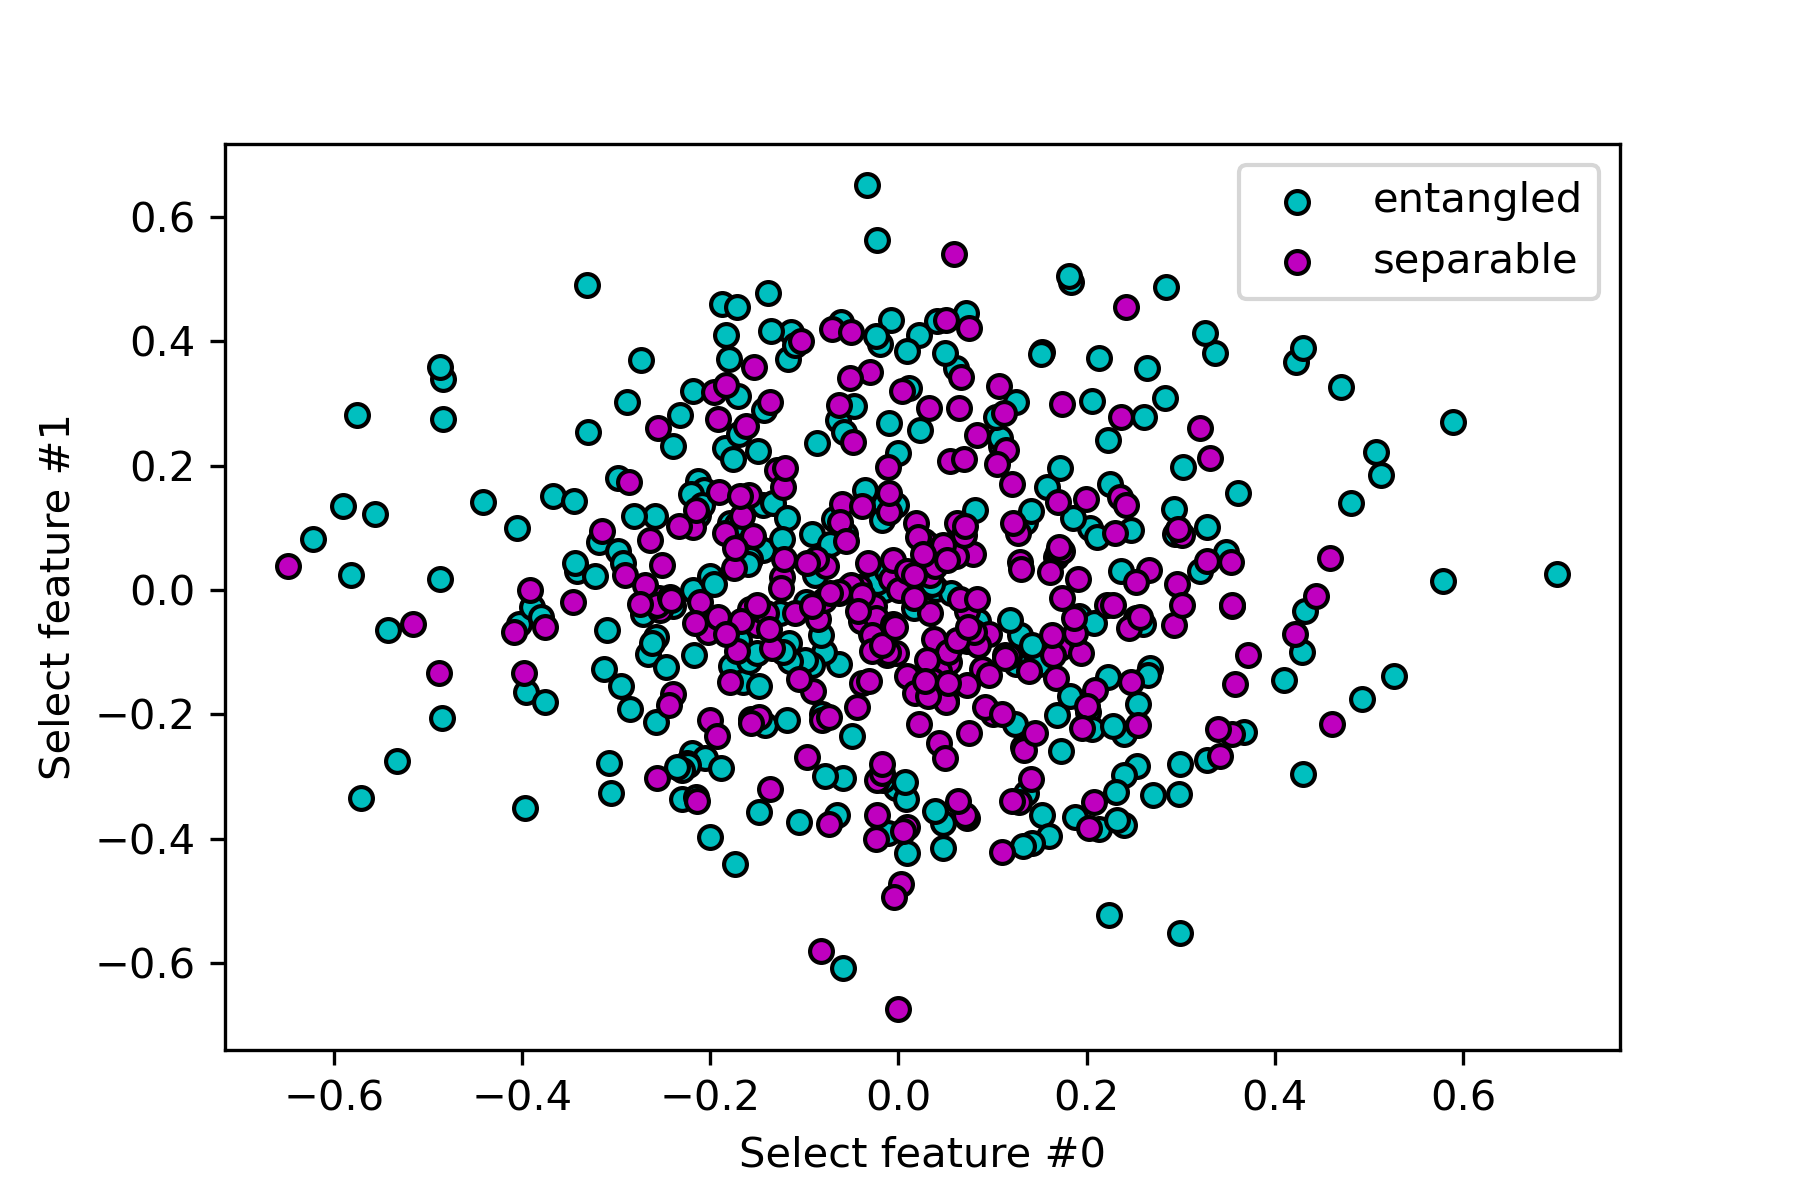
\includegraphics[width=.4\linewidth]{./notebook/feature_space_2.png}
% 	% 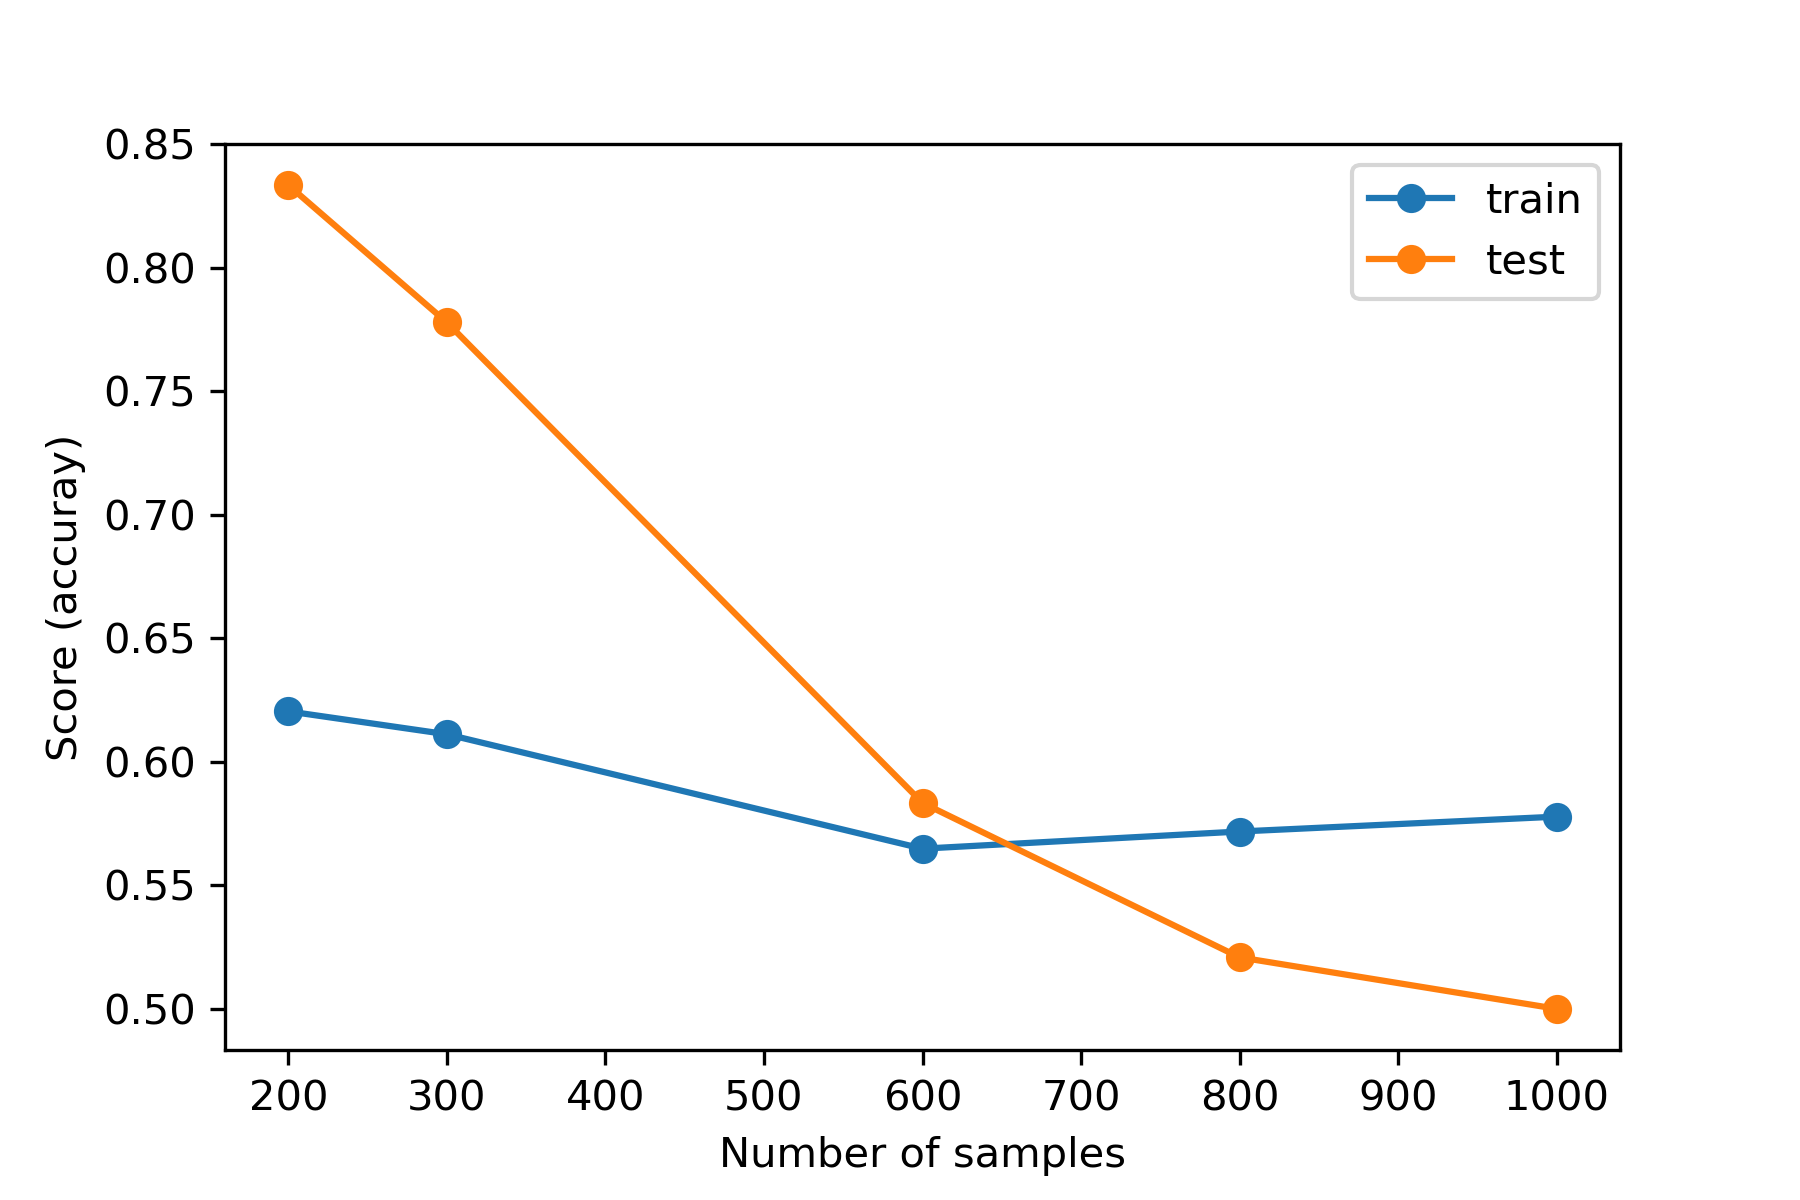
\includegraphics[width=.4\linewidth]{./Code/two_qubit_scores.png}
% 		% 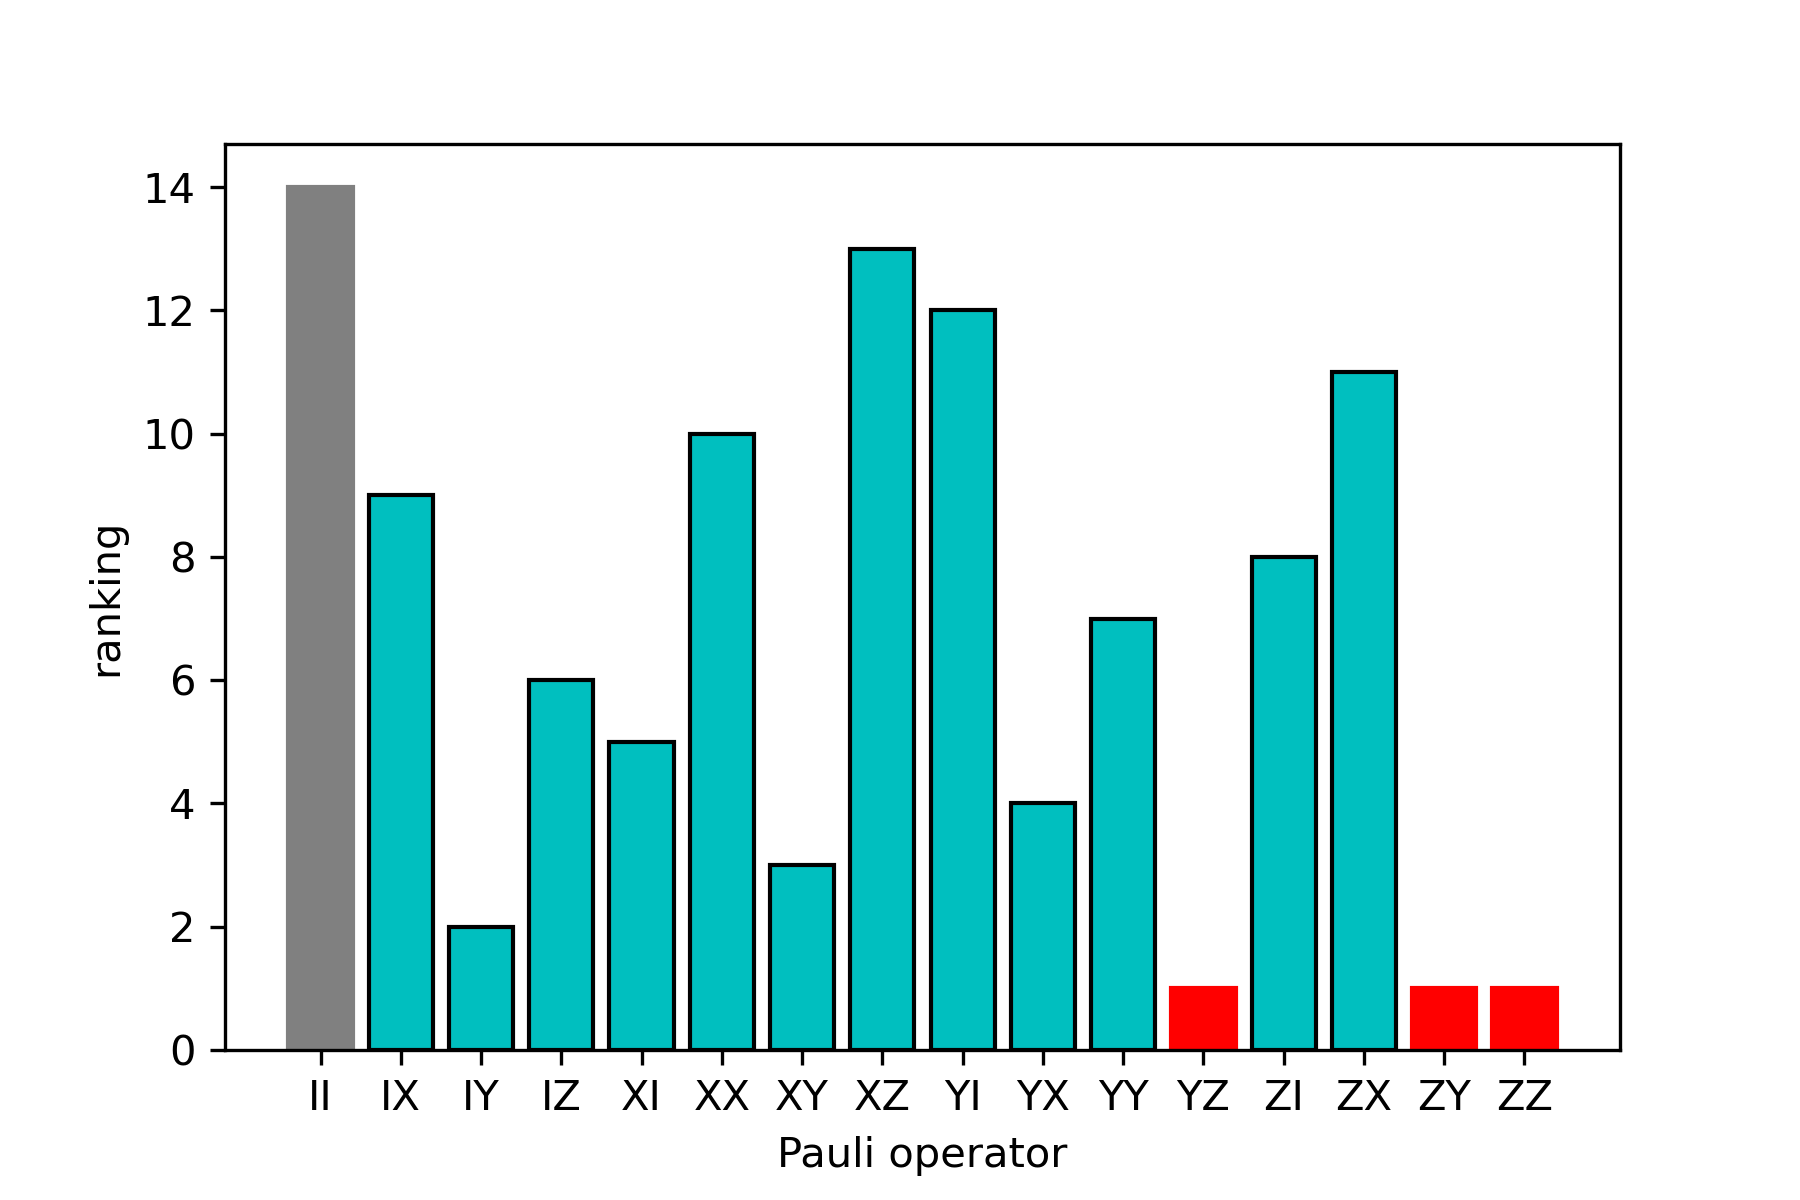
\includegraphics[width=.9\linewidth]{./Code/feature_rank.png}
% 		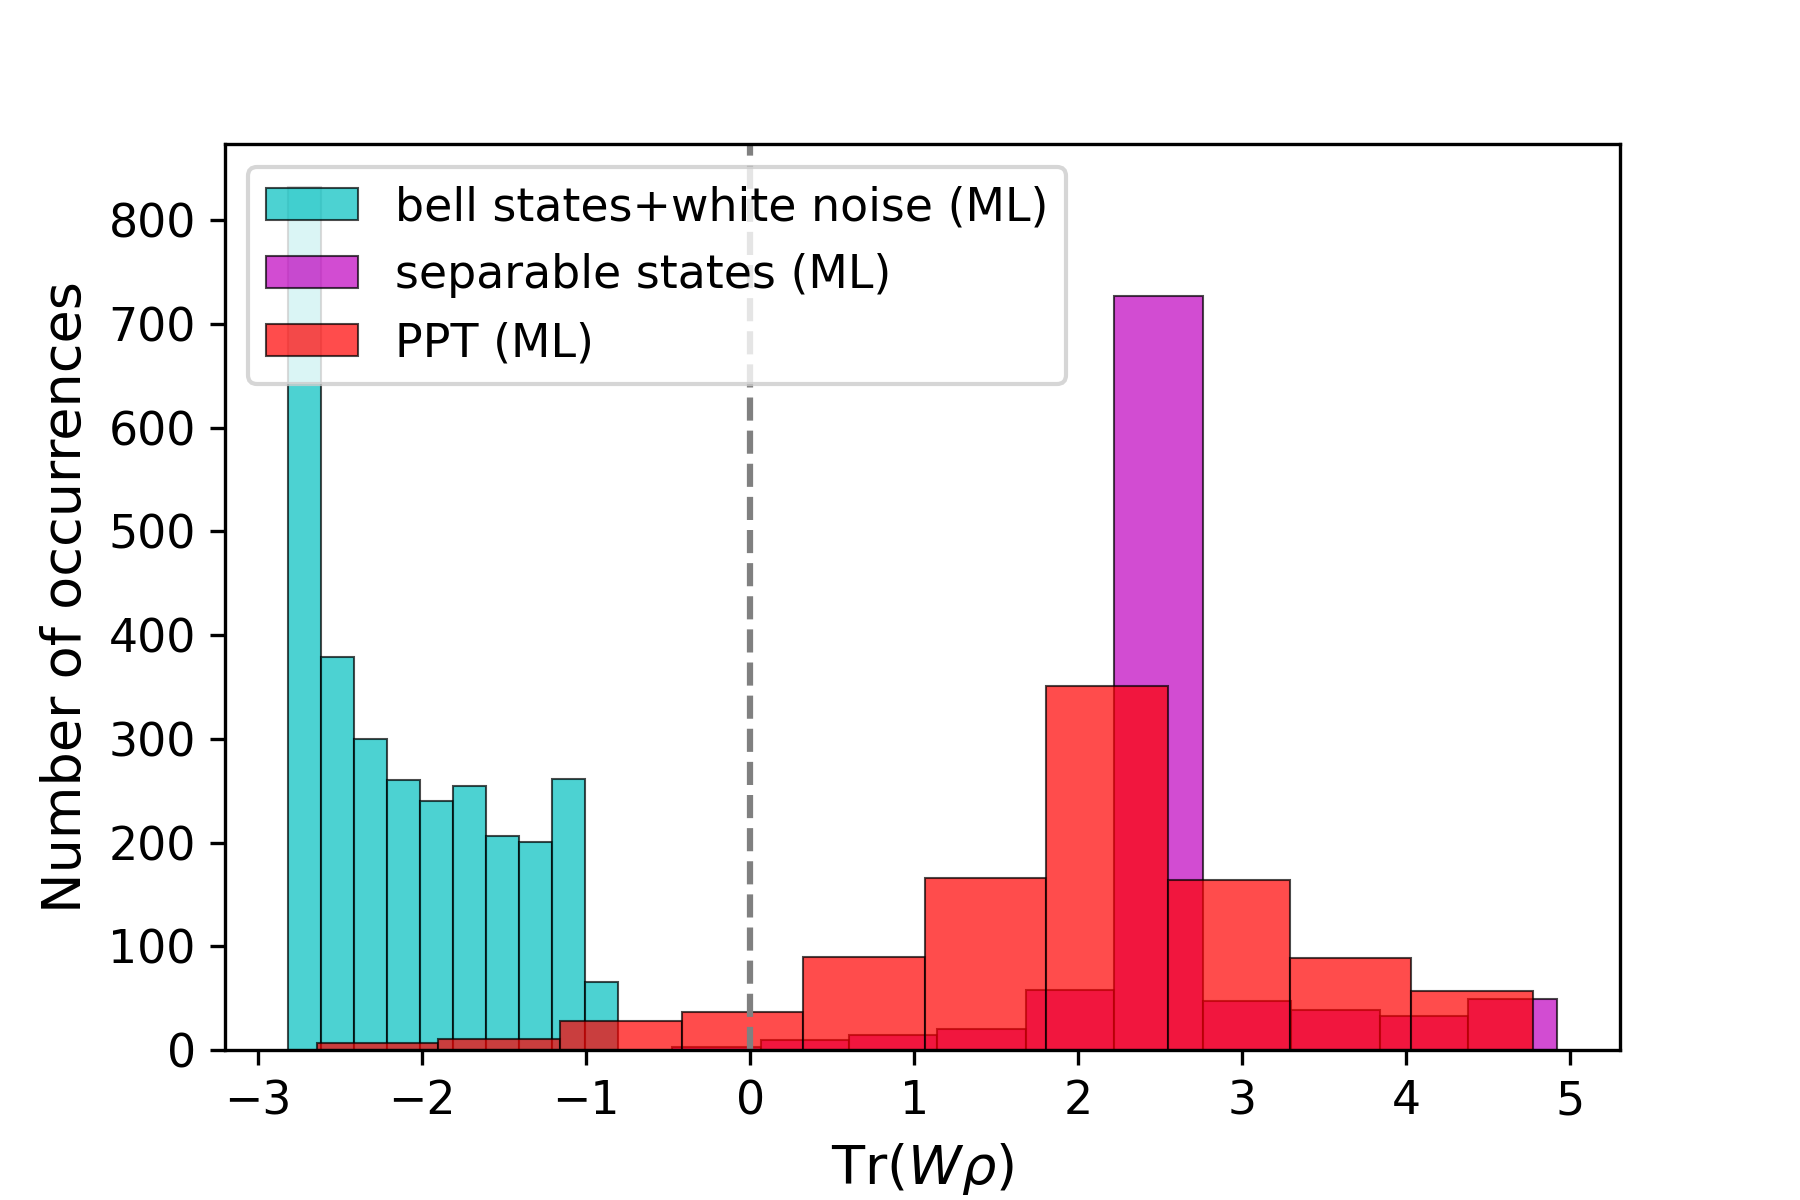
\includegraphics[width=.9\linewidth]{./Code/two_qubit_bell_ml.png}
	\subfloat{%
	% \subfloat[\label{subfig:a}]{%
		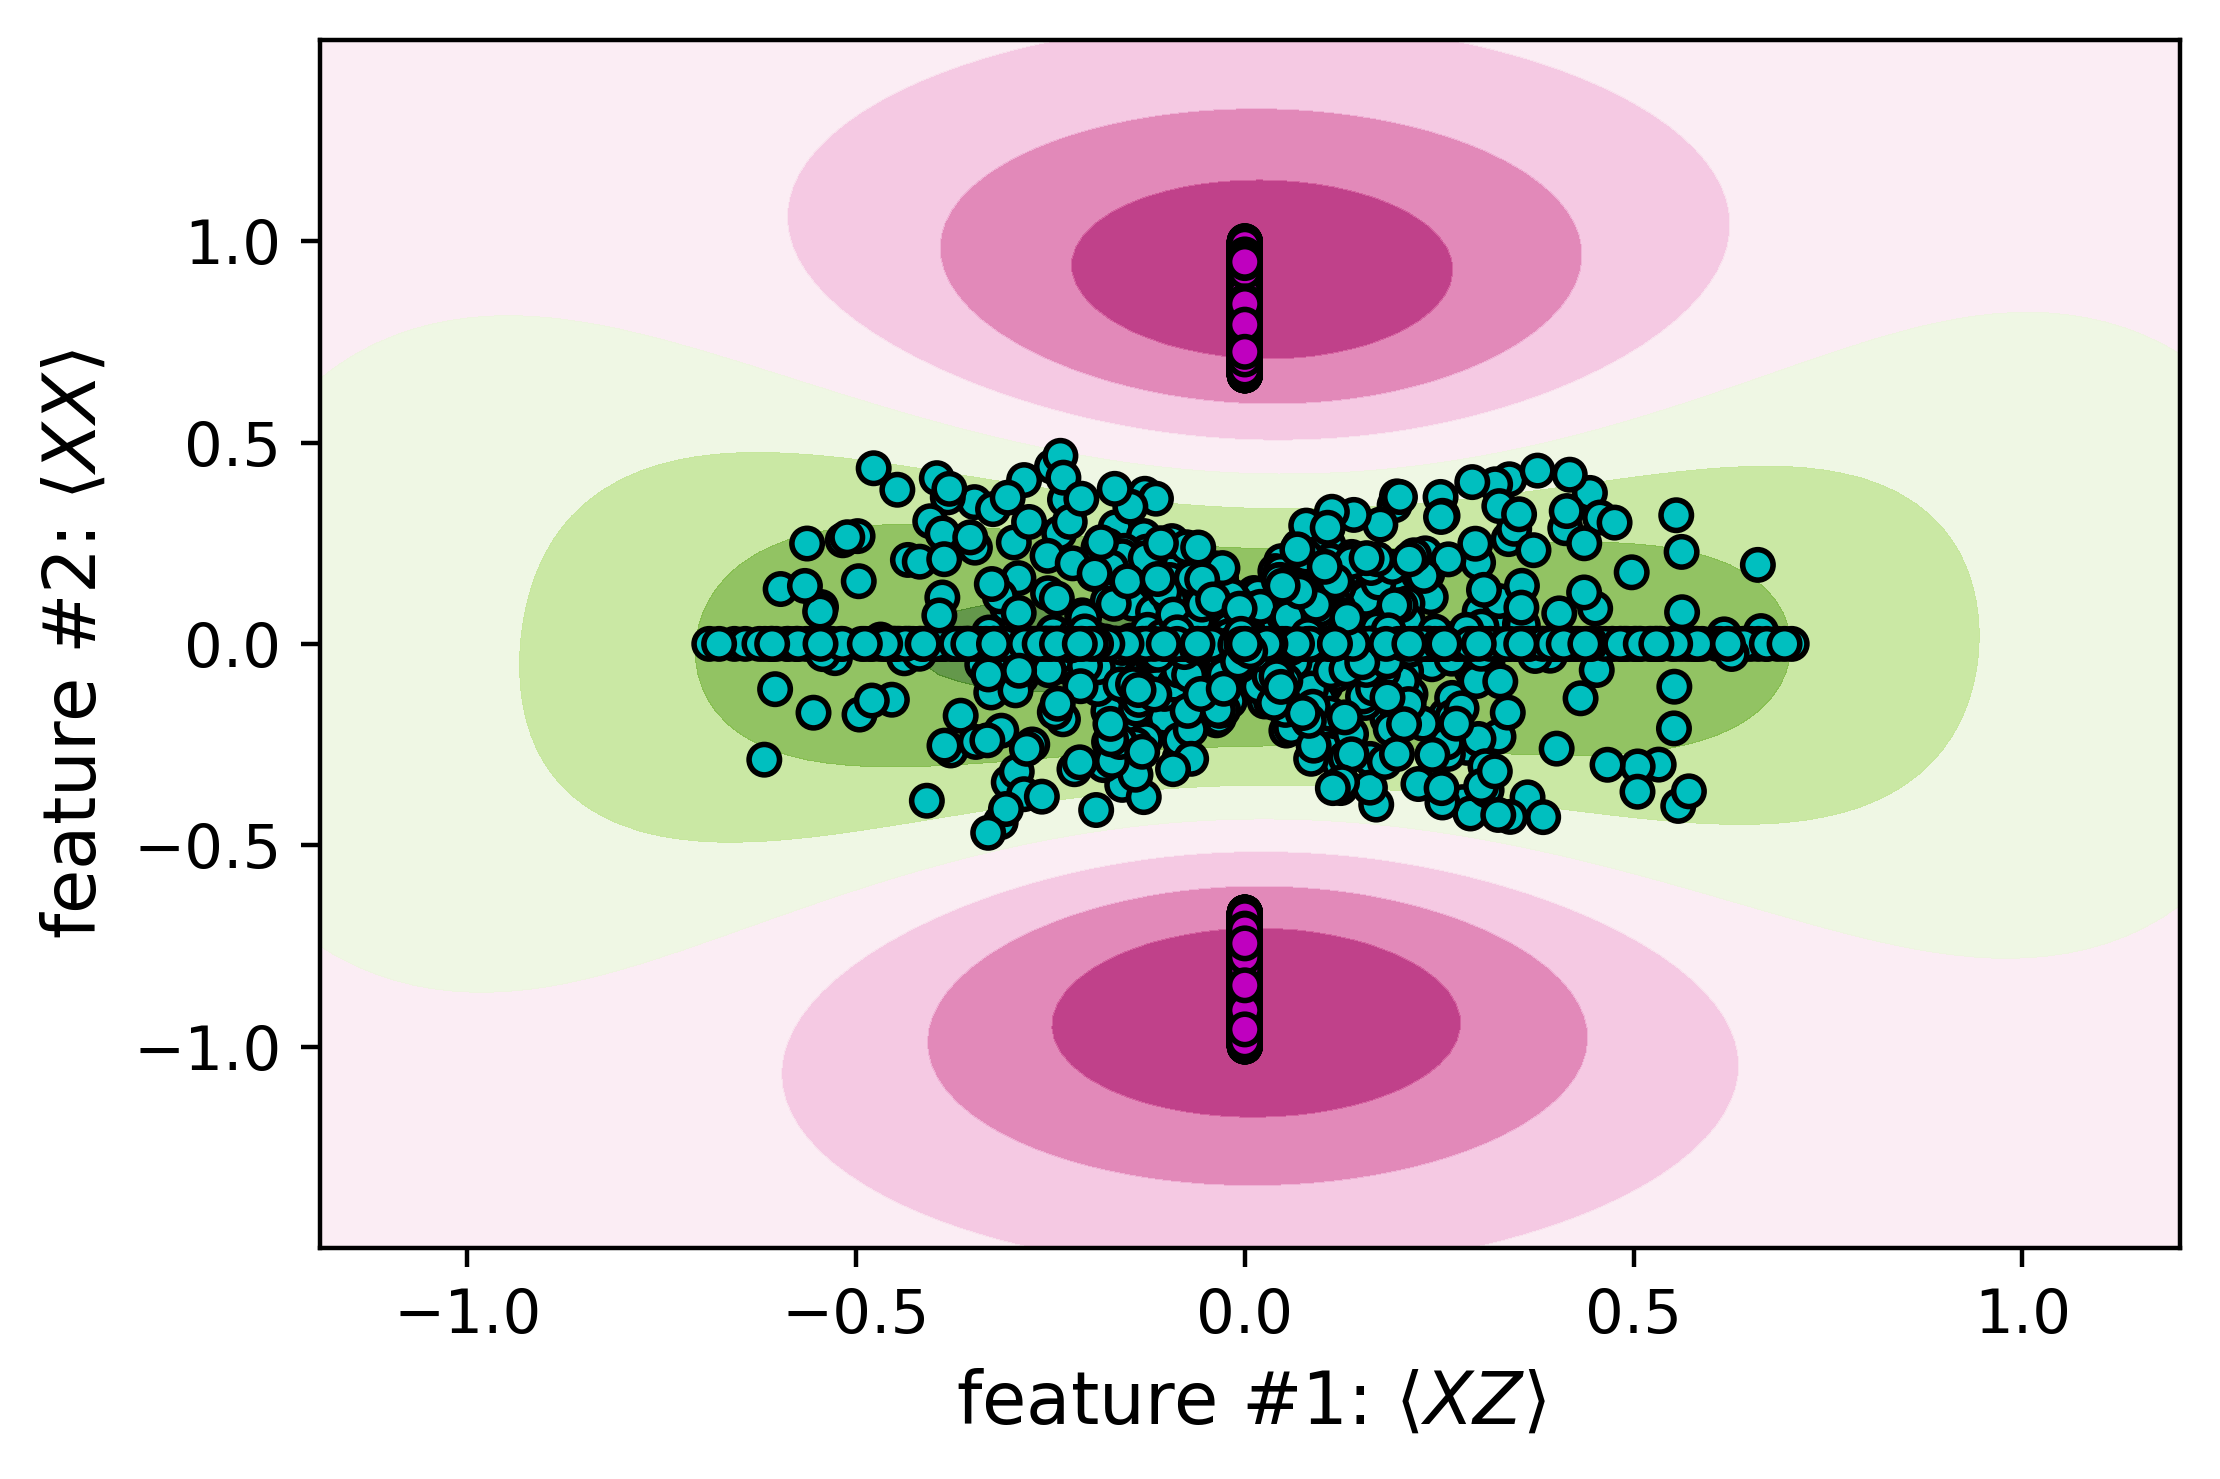
\includegraphics[width=.9\columnwidth]{./Code/feature_space_2d_XZ_XX_13.png}
	}\hfill
	\subfloat{%
		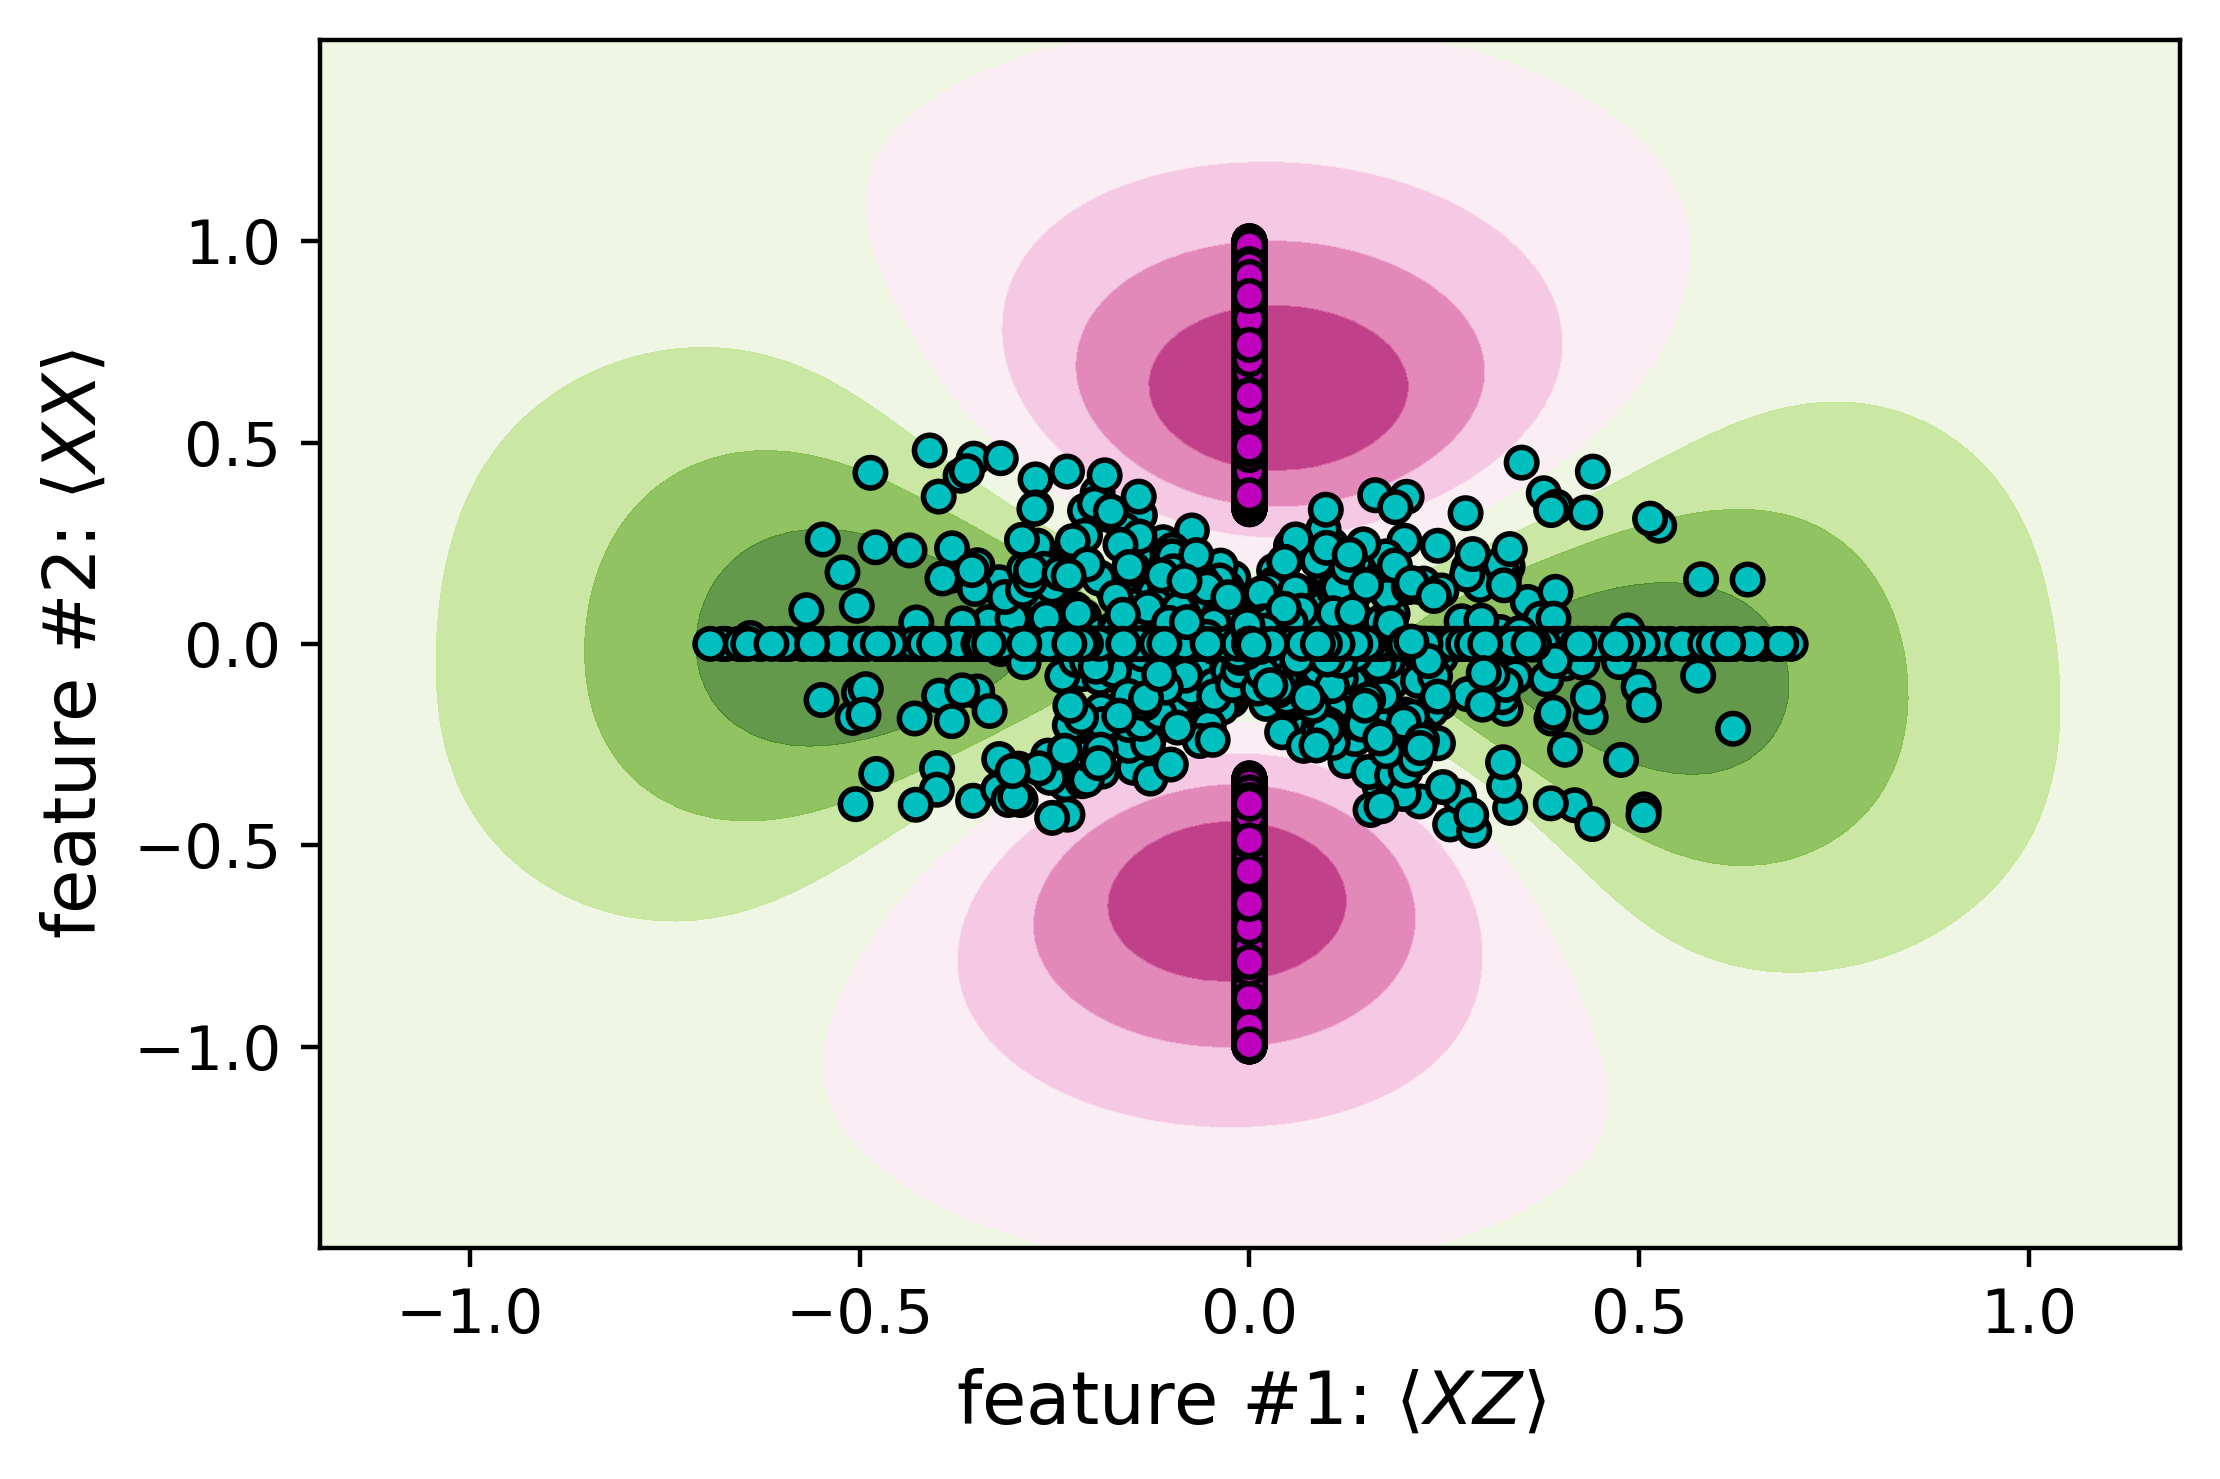
\includegraphics[width=.9\columnwidth]{./Code/feature_space_2d_XZ_XX_23.png}
	}
	\caption{The two-dimensional embedding (a low-dimensinoal feature space $\expval{XZ}$ VS $\expval{XX}$) of 2-qubit states: green dots represent randomly sampled separable states, while pink ones represent entangled Bell states mixed with white noise in the range (left figure) $p_{\noise}\in[0,1/3]$ and (right figure) $p_{\noise}\in[0,2/3]$. The colored shade indicates the nonlinear decision boundary of the RBF kernel SVM classifier. When the white noise is larger, the gap between two sets of data points is smaller such that training a classifier becomes harder.}
	% \caption{feature space, recursive feature elimination}
	\label{fig:feature_space}
\end{figure*}
A key drawback of conventional witnesses is its linearity because many real-world datasets are not linearly-separable in a low-dimensional feature space.
Despite the nonlinear witness \cite{guhneNonlinearEntanglementWitnesses2006} proposed, its experimental implementation is more challenging than linear ones.
The good news is,
within the framework of SVM, non-linearity can be easily achieved by the so-called kernel method \cite{hofmannKernelMethodsMachine2008}.
The main idea is mapping the features $\vbx$ to a higher dimensional space via a feature map $\phi(\vbx)$ such that they can be linearly separated in the high-dimensional feature space.
% the polynomial kernel $\kernel_{\text{poly}}(\vbx,\vbx') := (1+\vbx\cdot\vbx')^q$ with feature map $\phi(\vbx)$ ...
% An important feature of kernel method is that kernels can be computed efficiently without evaluating feature map (might be infinite dimension) explicitly.
The kernel function $\kernel(\vbx,\vbx'):\mathcal{X}\times \mathcal{X} \to \realnumber$ measures the similarity between two input data points in a high-dimensional feature space because a kernel can be written as an inner product $\langle \phi(\vbx),\phi(\vbx') \rangle$.
The commonly used kernel is the radial basis function (RBF) kernel which a Gaussian function
$\kernel_{\text{rbf}}(\vbx,\vbx') := \exp(-\gamma\norm{\vbx-\vbx'}^2_2)$ with $l_2$ Euclidean norm and a parameter $\gamma$.
Since the RBF kernel SVM is convex, the optimal classifier function will be found if it exists for the input dataset.
It can be easily observed in \cref{fig:feature_space} that two kinds of data points are clearly classified by a nonlinear (RBF kernel) SVM classifier, though it is not linearly separable in this 2-dimensional space.


% \subsubsection{Our witness ansatz and optimization}

\begin{table}[!ht]
	\centering
	\begin{tabular}{c|c|c|c}
		Witnesses & \# observables & weights & comment \\
		\hline
		% entanglement witness & & & known \\  
		Conventional fidelity   & few LMS & fixed & one-side  \\  
		% convex?\cite{chakrabartiQuantumAlgorithmsLower2020} 
% 		Bell (CHSH) inequality & constant & fixed & weak \\  
		% entangle spectrum \cite{horodeckiDirectDetectionQuantum2002} & & & unknown \\  
		\textbf{SVM (kernel) } &  $\ll 4^n-1$ & trained & flexible \\  
		Tomographic (NN)  & $4^n-1$ & trained & universal \\  
		\hline
	\end{tabular}
	\caption{Comparison of conventional fidelity witness, tomographic classifier, and SVM witness.}
	\label{tab:comparison}
\end{table}
We compare the characters of different kinds of witnesses in \cref{tab:comparison}. 
The conventional fidelity witness only need few local measurement settings for stabilizer states, but it is a one-side test. 
The tomographic witness trained by NN only need the promise that there is a gap between entangled and separable states (almost universal), but it requires complete information of a state ($4^n-1$ features).
Between these two cases, the SVM witness has stronger classification capability than conventional fidelity witnesses and do not need as many classical features as the tomgraphic witness.
However, these prior ML witnesses only consider the robustness to white noise and cannot be directly applied to experiments.
%  because they didn't address the problem of estimating classical features. 
In numerical simulation, we can efficiently evaluate classical features by direct calculation, 
but in actual experiments, entries of a density matrix are not explicitly known.
Instead, we need to estimate observables (classical features) by repeat measurements, which we are going to discuss in next section.


% \subsubsection{Variational entanglement witness (ansatz)}

\subsection{Sample-efficient expectation estimation methods}\label{sec:estimation}
% \subsection{Estimate classical features of quantum states}
% To apply classical machine learning classifier (SVM) in actual experiments, we need classical features of quantum states.
% Nevertheless, we cannot directly evaluate expectation values as in numerical simulation because we do not know density matrices of incoming states.
% \textbf{features}: classical shadow? raw data? quantum data, label: entangled?
% \subsection{Tomography and trace estimation}
% \label{sec:shadow_tomography}
The brute force approach to fully characterize a state in an experiment is quantum state tomography \cite{altepeterPhotonicStateTomography2005}
\footnote{Quantum state tomography refers to the task of recovering the density matrix of an unknown $D$-dimensional state $\dm$ within error tolerence $\epsilon$, 
given the ability to prepare and measure copies of $\dm$.}.
With a recovered densitry matrix, we can directly calculate classcial features or separability measures,
but full tomography is experimentally demanding.
% \begin{problem}[quantum state tomography]\label{prm:full_tomography}
% 	Informally, quantum state tomography refers to the task of estimating complete description (density matrix) of an unknown $D$-dimensional state $\dm$ within error tolerence $\epsilon$, 
% 	given the ability to prepare and measure copies of $\dm$.
% 	% measure $m$ copies $\dm^{\otimes m}$.
% 	% \begin{equation}\label{eq:stokes_tomography}
% 	% 	\dm = \frac{1}{2^n} \sum_{i_1,i_2,\dots,i_n=0}^3
% 	% 	S_{i_1,i_2,\dots,i_n} 
% 	% 	\hat{\sigma}_{i_1} \otimes \hat{\sigma}_{i_2} \otimes \dots \otimes \hat{\sigma}_{i_n} 
% 	% 	\begin{itemize}
% 	% 		\item \textbf{Input}: Given a \textbf{unknown} $N$-dimensional mixed state $\dm$
% 	% 		\item \textbf{Output}:
% 	% 	\end{itemize}
% 	% \end{equation}
% \end{problem}
% The canonical representation (decomposition) of a $n$-qubit density matrix
% is $\dm=2^{-n} \sum_{\bmsigma \in \qty{I,X,Y,Z}^n} t_{\bmsigma}  \ob_{\bmsigma} $  
% % is $\dm=2^{-n} \sum_{\vb{p}\in \qty{I,X,Y,Z}^n} t_{\vb{p}} \bigotimes_i^n \vb{p}$  
% \cite{altepeterPhotonicStateTomography2005}.
	% Stokes decomposition
% Since there are $D^2$ entries in a density matrix, navie full tomography based on independent measurements need at least $D^2$ copies.
Even adaptive or collective measurements (and post-processing) allowed 
\footnote{Adaptive measurements are the intermediate between independent measurements and collective (entangled) measurements, in which the copies of $\dm$ are measured individually, but the choice of measurement basis can change in response to earlier measurements.},
rigorous analysis \cite{haahSampleoptimalTomographyQuantum2017} \cite{odonnellEfficientQuantumTomography2016} showed that 
$\Omega(D^2/\epsilon^2)$ measurements (copies)  are required for recovering a $D\times D$ density matrix
% $\Omega(Dr/\epsilon^2)/\log(D/r\epsilon)$ copies/measurements are required for a $D$-dimensional ($D=2^n$ for $n$-qubit systems), rank-$r$ density matrix 
with error tolerence $\epsilon$ measured by trace distance.
% \begin{problem}[Fidelity estimate]
% 	defined as follows
% 	\begin{itemize}
% 		\item \textbf{Input}: Given two density matrices $\dm$ and $\dm'$, 
% 		\item \textbf{Output}: \nameref{def:fidelity} with error $\epsilon$
% 	\end{itemize}
% \end{problem}
Now that full tomography is intractable for large systems, a workaround is to extract (partial) information about a state without fully recovering it:
% The answer is yes.
% \begin{problem}[trace estimation]\label{prm:trace_estimation}
% 	related problems defined as follows
% 	\begin{itemize}
% 		\item \textbf{Input}: Given an observable (Hermitian) $\ob$ and (copies of) a mixed state $\dm$ or several states ($\dm',\dots,\dm_m$), 
% 		\item \textbf{Output}: 
% 		with error $\epsilon$ measured by trace \nameref{def:distance} (\nameref{def:fidelity}...), to estimate
% 		linear functions (mostly): the expectation value $\expval{\ob}=\Tr(\ob \dm) $, entanglement witness, tomography; 
% 		nonlinear functions: \nameref{def:entropy};
% 		multivariate functions:  $\Tr(\dm_1 \cdots \dm_m)$, \nameref{def:quantum_kernel} $\Tr(\dm\dm')$,  quadratic $\Tr(\ob \dm_i \otimes \dm_j)$, \nameref{def:fidelity} $F(\dm,\dm')$, \nameref{def:distance}??;
% 	\end{itemize}
% \end{problem}
% Nevertheless, we usually only need specific properties of a target state rather than full classical descriptions about the state.
% this enables the possibility to \emph{shadow tomography} \cite{aaronsonShadowTomographyQuantum2018}:
\begin{problem}[shadow tomography]\label{prm:shadow_tomography}
	% Aaronson's formulation	
	Given $m$ copies (samples) of an unknown $D$-dimensional state and $M$ known 2-outcome measurements $\qty{E_1,\dots,E_M}$,
	to estimate $\forall i,\Tr(\dm E_i)$ within additive error $\epsilon$ with success probability at least $1-\delta$.
	% \hfill
	% \begin{itemize}
	% 	\item \textbf{Input}: $m$ copies of an unknown $D$-dimensional state and $M$ known 2-outcome measurements $\qty{E_1,\dots,E_M}$,
	% 	% each of which accepcts $\dm$ with probability $\Tr(E_i \dm)$ and rejects with probability $1-\Tr(E_i \dm)$
	% 	\item \textbf{Output}: estimation of $\Tr(\dm E_i)$ within additive error $\epsilon$, $\forall i\in [M]$, with success probability at least $1-\delta$.	
	% \end{itemize}
\end{problem}
% \begin{theorem}[\cite{aaronsonShadowTomographyQuantum2018}]\label{thm:shadow_tomography}
% 	It is possible to do \nameref{prm:shadow_tomography} using $\tilde{\bigO}(\log^4 M\cdot \log D\cdot\epsilon^{-4})$ copies
% 	\footnote{full tomography: additive error $\epsilon\ll 1/D$.}.
% 	sample complexity lower bound $\Omega(\log (M) \cdot \epsilon^{-2})$, 
% \end{theorem}
% \begin{theorem}[lower bound of \nameref{prm:full_tomography}?\cite{haahSampleoptimalTomographyQuantum2017}]
	% Though formally “efficient” in the sense that $N$ scales polynomially with $m$ for any fixed approximation error $\epsilon$, 
% \end{theorem}
Since shadow tomography can be implemented with $\tilde{\bigO}(\log^4 M\cdot \log D\cdot \log 1/\delta \cdot\epsilon^{-4})$ copies \footnote{$\tilde{\bigO}$ hides a polylog factor. A full tomography require estimate $D^2$ measuremments (observables) with additive error $\epsilon\ll 1/D$ for all $E_i$, so the sample complexity of shadow tomography is compatiable with lower bounds of full quantum state tomography.} \cite{aaronsonShadowTomographyQuantum2018},
we can estimate $M$ classical features (Pauli observables) for $f(\vbx_{\dm,\tilde{\bmsigma}})$ in a samples-efficient manner.
% \footnote{nonlinear functions: von Neumann entropy $\Tr(\dm\log(\dm))$;
% multivariate functions:  $\Tr(\dm_1 \cdots \dm_m)$, fidelity (quantum kernel?) $\Tr(\dm\dm')$,  quadratic $\Tr(\ob \dm_i \otimes \dm_j)$.},
However, Aaronson's shadow tomography procedure is very demanding in terms of quantum hardware (in the collective preparation and measurement on $\dm^{\otimes m}$).
To be more feasible for current experiments, Huang et. al \cite{huangPredictingManyProperties2020} introduced classical shadow (CS) scheme which we apply in our protocol.
% \begin{remark}[compare shadow tomography with classical shadow \cite{huangPredictingManyProperties2020}]
% 	While very efficient in terms of samples, Aaronson's procedure is very demanding in terms of quantum hardware - a concrete implementation of the proposed protocol requires \textbf{exponentially long quantum circuits} that act collectively on all the copies of the unknown state stored in a quantum memory.
% 	% [compare shadow tomography and classical shadow ??]
% \end{remark}
% \subsubsection{Estimate expectations via classical shadow}\label{sec:classical_shadow}

% much like Monte Carlo sampling approximates an integral.
	% \begin{equation}
	% 	o_i = \Tr(O_i \dm_{\cs})
	% 	\text{ obeys }
	% 	\expectation[o_i] =\Tr(O_i \dm).
	% \end{equation}
% \nameref{def:classical_shadow} \cite{huangPredictingManyProperties2020}: estimate entanglment witness (fixed but unknown target state, e.g., tripartite GHZ)
% \textbf{Classical shadows (Clifford measurements) of logarithmic size allow for checking a large number of potential entanglement witnesses simultaneously}.
% Directly measuring $M$ different entanglement witnesses requires a number of quantum measurements that scales (at least) linearly in $M$. In contrast, classical shadows get by with $\log(M)$-many measurements only.
% classical shadows are based on random Clifford measurements and do not depend on the structure of the concrete witness in question. In contrast, direct estimation crucially depends on the concrete witness in question and may be considerably more difficult to implement. \cite{huangPredictingManyProperties2020}
% The transformation $U$ is randomly selected from an ensemble of unitaries, and different ensembles lead to different versions of the procedure that have characteristic strengths and weaknesses.

% more details in \cref{sec:classical_shadow}

% \begin{definition}[classical shadow]\label{def:classical_shadow}
% 	The classical shadow of a state $\dm$ is a ...
% 	such that we can predict the linear function with it
% 	\begin{equation}
% 		o_i = \Tr(O_i \dm_{\cs})
% 		\text{ obeys }
% 		\expectation[o] =\Tr(O_i \dm)
% 	\end{equation}
% \end{definition}

% \begin{algorithm}[H]
%     \DontPrintSemicolon
%     \SetKwInOut{Input}{input}
%     \SetKwInOut{Output}{output}
%     \Input{(copies of) density matrix $\dm$, an entanglement witness (observable) $\ew$}
%     \Output{$\Tr(P_x \dm ), \forall x \in \qty{ I, X, Y, Z }^n$}
%     \BlankLine
%     % \For{ $i = 1,2, \ldots, m$} {
%     %     $P_x$  \tcp*{estimate entanglement witness by quantum ML}
%     %     % \tcc{comment in a new line}
%     % % {\Return $\Tr(\ew\dm)$ }
%     % }
%     \Return estimation of $\Tr(\ew\dm)$ 
%     % \Return entangled ? GME ? separable with certain partition?
%     \caption{features for \nameref{def:entanglement_witness}}
%     \label{alg:entanglement_witness}
% \end{algorithm}
\begin{algorithm}[H]
    \DontPrintSemicolon
    \SetKwInOut{Input}{input}
    \SetKwInOut{Output}{output}
    \Input{$R$ copies of $\dm$ and selected observables $\pob_{\tilde{\bmsigma}}$}
	% (black-box access to a circuit preparing a state)
	% , observables $\ob$...
    \Output{estimation of $\vbx_{\dm,\tilde{\bmsigma}}:=\Tr(\dm\pob_{\tilde{\bmsigma}})$}
    % \Output{\nameref{def:classical_shadow} $\dm_{cs}$}
    \BlankLine
	Sample $R$ Pauli measurements $P\in\qty{X,Y,Z}^{\otimes n}$ \\
	% \tcp{assume $n$-qubit state $\dm$}
    \For{ $i = 1,2, \ldots, R$} {
		\tcp{apply single-copy measurement $P$ to a copy $\dm$} 
        $\dm\mapsto \U_P\dm \U_P^\dagger\mapsto \ket{\vb{b}}$ with $b_j\in \qty{0,1},\forall j\in[n]$ \\
		% \tcp*{apply a random unitary}
		% $\ket{b}\in \qty{0,1}^n $ \tcp*{measure in computational basis}
		\tcp{inverse channel $\mathcal{M}^{-1}(\dm')=(3\dm'-I)$}
		$\dm_{\cs}^{(i)}=\bigotimes_j \qty(3U_j^\dagger \op{b_j} U_j-I)$ 
		% $\dm_{\cs}=\mathcal{M}^{-1}\qty(\U^\dagger \op{b} \U)$ \tcp*{$\mathcal{M}$ quantum channel}
        % \tcc{comment in a new line}
    % {\Return ?}
    }
    $\text{CS}(\dm,R)=\qty{\dm_{\cs}^{(1)},\dots,\dm_{\cs}^{(R)}}$ \tcp*{classical shadow}
	\tcp{estimate features for SVM from classical shadow}
	\Return  $\vbx_{\dm,\tilde{\bmsigma}}=\textsc{Expectation}(\text{CS}(\dm,R)O_{\tilde{\bmsigma}})$
    \caption{estimate Pauli observables by randomized classical feature}
    \label{alg:classical_shadow}
\end{algorithm}
The classical shadow of a state $\dm$ (a set of snapshots $\dm_{\cs}$) is a succinct classical description of a state $\dm$, which can be used to estimate the expectations of a sef of observables with a reasonably small number of copies of the state.
To construct the randomized classical shadow, we firstly need to uniformly sample $R$ Pauli measurements $P\in\qty{X,Y,Z}^{\otimes n}$ (assume the state $\dm$ of $n$ qubits).
Then, we apply single-copy measurement $P$ to a copy of $\dm$, i.e., each measurement measures all qubits in Pauli $X$, $Y$, or $Z$-basis according to $P$.
Specifically, we apply the transformation $\dm \mapsto \U \dm \U^\dagger$ where $U^\dagger P U = \Sigma$ is the eigendecomposition of $P$ and then measure this rotated stated in computational basis (collapse to $\ket{\vb{b}}\in\qty{\ket{0},\ket{1}}^{\otimes n}$).
% extracted by performing reasonably simple single-copy measurements 
The expectation values of a set of observables can be approximated 
A snapshot $\dm_{\cs}$ can be constructed by taking the inverse of the quantum channel $\mathcal{M}^{-1}(U^\dagger\op{\vb{b}}U)$.
By repeating this procedure $R$ times, we obtain $R$ snapshots of $\dm$ which can be used to estimate the expectation values of a Pauli observable by an empirical average over $R$ classical shadows, 
i.e., $o = \Tr(O \dm_{\cs})$ obeys $\expectation[o] =\Tr(O \dm)$.
% \begin{equation}
% % 	\dm_{\cs} := \mathcal{M}^{-1} \qty(U^\dagger \op{b} U),
% 	\dm_{\cs} := \bigotimes_j \qty(3U_j^\dagger \op{b_j} U_j-I),
% \end{equation}
% where $\mathcal{M}=$.
The algorithm is summarized in Algorithm. \ref{alg:classical_shadow}.

The size of the classical shadow scales $\bigO(\log(M) 3^k/\epsilon^2)$ to approximate $M$ $k$-local Pauli observables with error tolerance $\epsilon$ \cite{huangPredictingManyProperties2020},
so this scheme has advantage the small $k$ and large $M$ (many quite local observables).
% but is independent of the number of qubits
% \footnote{Known fundamental lower bounds state that classical shadows of exponential size (at least) $T = \Omega( 2^n / \epsilon^2)$ are required to $\epsilon$-approximate $\dm$ in trace distance.}
% \footnote{ $\Omega(\log(M) 3^k/\epsilon^2)$ lower bound ??}
% \subsubsection{Derandomization}
There are several variants of classical shadow method \cite{hadfieldMeasurementsQuantumHamiltonians2022, huangEfficientEstimationPauli2021, chenRobustShadowEstimation2021}.
The derandomized version \cite{huangEfficientEstimationPauli2021} is the refinement of the original randomized protocol which provides better performance for $k$-local observables. 
The core idea of derandomized version is to select more Pauli measurements compatiable with $k$-local Pauli observables to be estimated.
The main result of this work is a procedure for identifying “good” Pauli measurements that allow for accurately predicting many (fixed) Pauli expectation values. This procedure is designed to interpolate between two extremes: (i) completely randomized measurements (good for predicting many local observables) and (ii) completely deterministic measurements that directly measure observables sequentially (good for predicting few global observables).
From the perspective of entanglement witness, the classical shadow method finds a effective local measurement settings for a sets of $k$-local Pauli observables.
% but not guarantees better performance for global observables (involving all subsystems).  
% noise-resilient variant \cite{chenRobustShadowEstimation2021} ...
The entanglement detection by estimating $p_3$-PPT with classical shadow \cite{elbenMixedstateEntanglementLocal2020} and comparison of classical shadow methods \cite{zhangExperimentalQuantumState2021} have been done experimentally.
% Similar to the PPT condition, the $p_3$-PPT condition (without full tomography) applies to mixed states and is completely independent of the state in question \cite{elbenMixedstateEntanglementLocal2020}. 
% \begin{figure}[!ht]
% 	\centering
% 	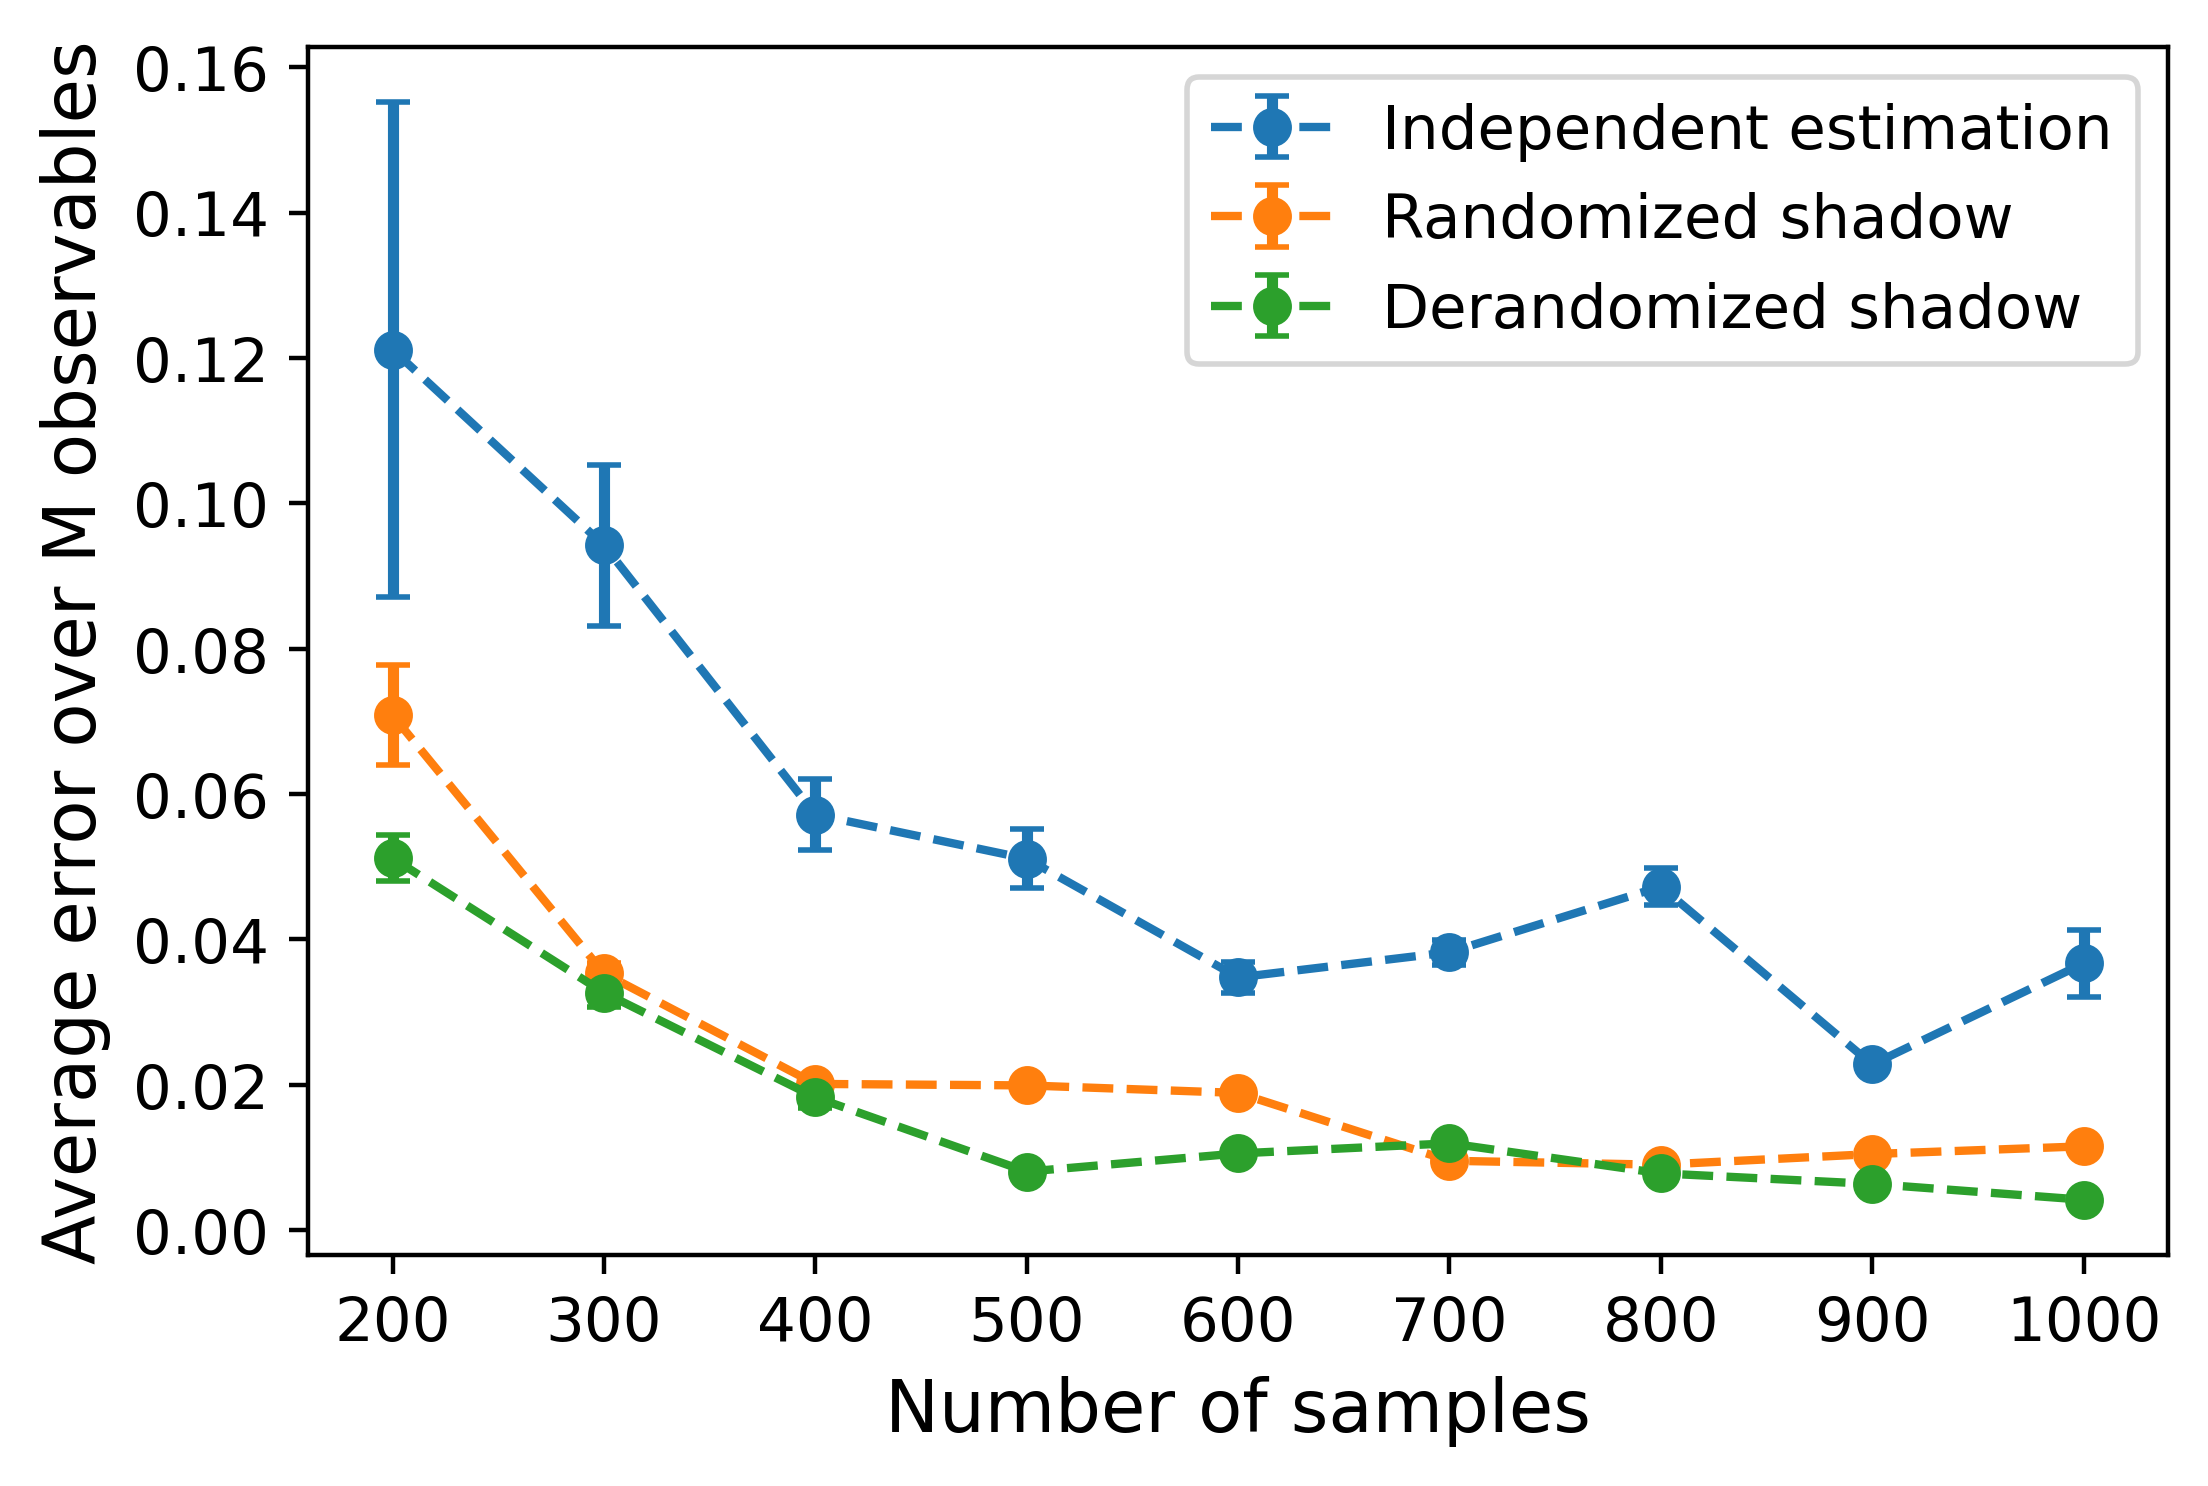
\includegraphics[width=.9\linewidth]{./Code/estimation_error_compare_methods.png}
% 	\caption{Error of estimating expectation values VS classical shadow sizes (number of samples)}
% 	\label{fig:shadow}
% \end{figure}
% \begin{lemma}
% 	predict linear function with shadow shadow:
% 	the variance
% 	\begin{equation}
% 		\variance[o] = \expectation[(o-\expectation[o])^2]
% 		\le \norm{O - \frac{\Tr(O)}{2^n} \identity}^2_{\shadow}
% 	\end{equation}
% \end{lemma}
% \begin{theorem}\label{thm:classical_shadow_upper}
% 	Fix a measurement primitive $\mathcal{U}$??, a collection $\qty{\ob_1,\dots,\ob_M}$ of $2^n\times 2^n$ Hermitian matrices and accuracy parameters $\epsilon,\delta\in[0,1]$.
% 	Set 
% 	\begin{equation}
% 		K = 2\log (2M/\delta)
% 		,\quad
% 		N = \frac{34}{\epsilon^2}\max_{1\le i\le M} \norm{\ob_i-\frac{\Tr(O_i)}{2^n} \identity}^2_{\shadow}
% 	\end{equation}
% 	where $\norm{\cdot}_{\shadow}$ is \nameref{def:shadow_norm}. 
% 	Then, a collection of NK independent classical shadows allow for accurately predicting all features via median of means prediction
% 	\begin{equation}
% 		\abs{o_i (N,K), -\Tr(O_i \dm)}\le \epsilon,\; \forall i\le i \le M
% 	\end{equation}
% 	wieth probability at least $1-\delta$.
% 	$o_i(N,K)=\textup{median}\qty{\Tr(\ob_i\dm_{(1)}),\dots,\Tr(\ob_i\dm_{(K)})}$
% 	% sample complexity
% 	% \begin{equation}
% 	% 	N_{tot} = \bigO \qty(
% 	% 		\frac{\log (M)}{\epsilon^2} \max_{1\le i\le M} 
% 	% 		\norm{O_i - \frac{\Tr(O_i)}{2^n} \identity}^2_{\shadow}
% 	% 	)
% 	% \end{equation}
% \end{theorem}
% \begin{definition}[shadow norm]\label{def:shadow_norm}
% 	$\norm{\cdot}_{\shadow}$ is shadow norm that only depends on the measurement primitive:
% 	\begin{equation}
% 		\norm{O}_{\shadow} =\max_{\sigma:state} \qty(
% 			\expectation_{U\sim \mathcal{U}}
% 			\sum_{b\in \qty{0,1}^n } \mel{b}{\U\sigma\U^\dagger}{b} 
% 			\mel{b}{\U\mathcal{M}^{-1}(O) \U^\dagger}{b}^2 
% 		)^{1/2}
% 	\end{equation}
% 	(nonnegative, homogeneous, triangle inequality)
% \end{definition}

% \begin{theorem}[\cite{huangPredictingManyProperties2020}]\label{thm:classical_shadow}
% 	Any procedure based on a fixed set of single-copy local measurements that can predict,
% 	with additive error $\epsilon$, $M$ arbitrary $k$-local linear function $\Tr(\ob_i\dm)$,
% 	requires at least (lower bound)
% 	$\Omega(\log(M) 3^k/\epsilon^2)$ copies of the state $\dm$.
% 	\footnote{Known fundamental lower bounds state that classical shadows of exponential size (at least) $T = \Omega( 2^n / \epsilon^2)$ are required to $\epsilon$-approximate $\dm$ in trace \nameref{def:distance}.}
% 	% \cite{huangProvablyEfficientMachine2022}
% 	$\Omega(\log(M) \max_i\Tr(\ob_i^2)/\epsilon^2)$ 
% \end{theorem}
% Consider a simple family of entanglement witnesses with compatible structure:  (ansatz??)
% \begin{equation}
% 	O:= O(V_A,V_B,V_C)=V_A\otimes V_B \otimes V_C \op{\psi_{\ghz}^+} V_A^\dagger\otimes V_B^\dagger \otimes V_C^\dagger
% \end{equation}
% the single-qubit unitaries $V_A,V_B,V_C$ parametrize differenet witnesses.



% \subsubsection{training data and classical kernel methods}
% $\sigma_T(\dm(x_l))$ is the classical shadow representation of $\dm(x_l)$, 
% a $2^n\times 2^n$ matrix that reproduces $\dm(x_l)$ in expectation over random Pauli measurements.
% \begin{equation}
% 	\qty{x_l\to\sigma_T(\dm(x_l))}_{l=1}^N
% \end{equation}

% \begin{definition}[shadow kernel]\label{def:shadow_kernel}
% 	given two density matrices (quantum states) $\rho$ and $\rho'$,
% 	\emph{shadow kernel} \cite{huangPredictingManyProperties2020} is 
% 	\begin{equation}
% 		k_{\shadow}(S_T(\dm),S_T'(\dm')) := 
% 		\exp( \frac{\tau}{T^2}
% 			\sum_{t,t'=1}^{T} \exp( \frac{\gamma}{n} 
% 			\sum_{i=1}^n \Tr(\sigma_i^{(t)}\sigma_i^{(t')}) ) 
% 			)
% 	\end{equation}	
% 	where $S_T(\dm)$ is the classical shadow representation of $\dm$.
% 	The computation time for the inner product is $\bigO(nT^2)$,
% 	linear in the system size $n$ and quadratic in $T$,
% 	the number of copies of each quantum state which are measured to construct the classical shadow.
% \end{definition}

% \begin{figure}[!ht]
% 	\centering
% 	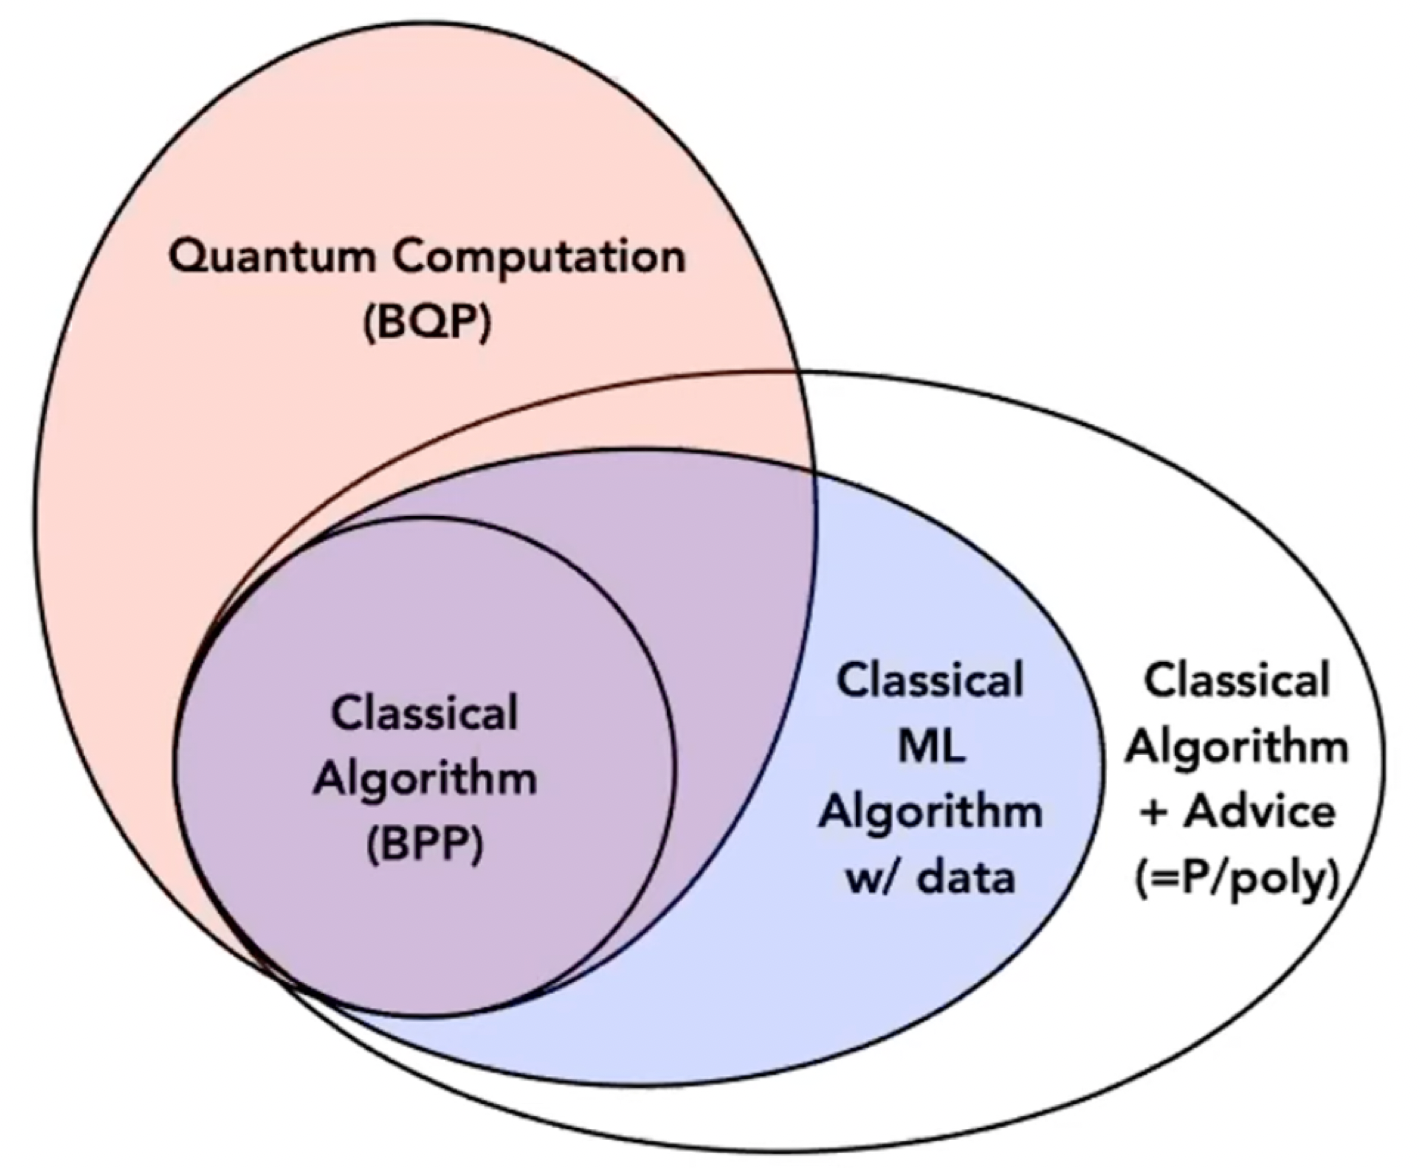
\includegraphics[scale=.2]{data.png}
% 	% 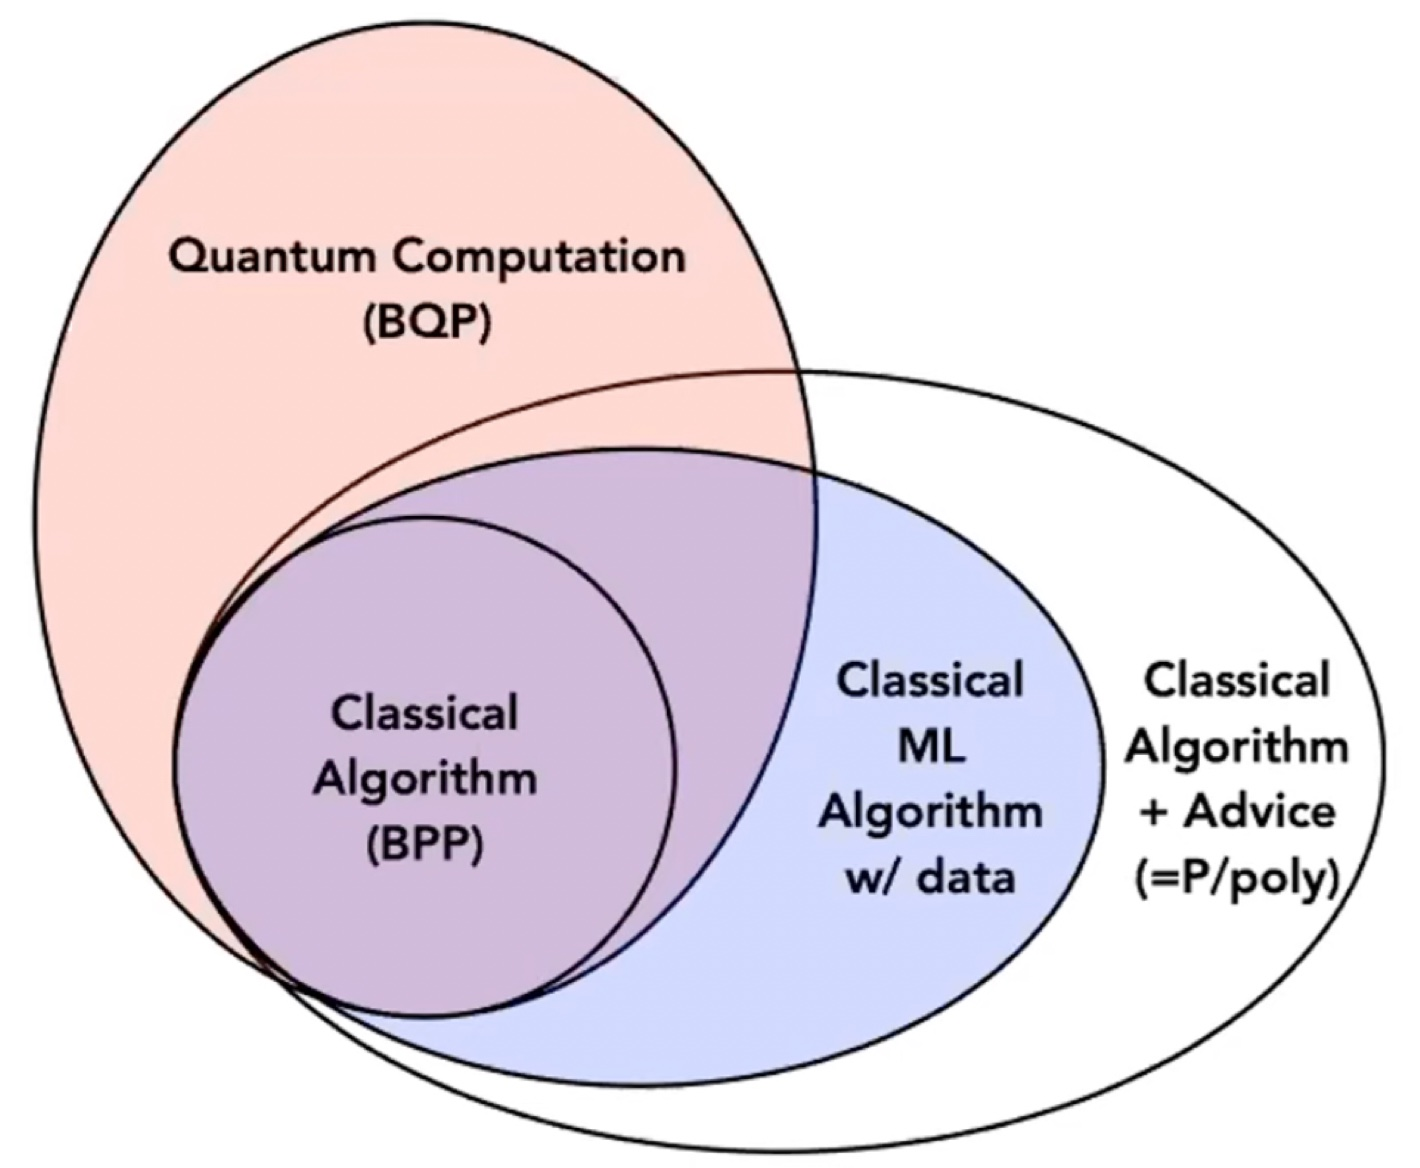
\includegraphics[width=.35\linewidth]{data.jpg}
% 	\caption{computational model powered by training data}
% \end{figure}

% \begin{proposition}[\cite{huangPowerDataQuantum2021}]
% 	exist quantum advantage in machine learning (not significant, practical)	...
% 	discrete log, factoring...
% \end{proposition}
% \begin{theorem}[informal \cite{huangPowerDataQuantum2021}]
% 	data learning
% 	\begin{itemize}
% 		\item machine learning (strictly) more powerful than BPP
% 		\item exist quantum advantage in machine learning (not significant, practical)
% 	\end{itemize}
% \end{theorem}

% \subsubsection{Estimate entanglement witness by (quantum) machine learning}
% though, that while there is no large advantage in query complexity, a substantial quantum advantage in computational complexity is possible.

% \begin{theorem}[\cite{huangInformationtheoreticBoundsQuantum2021}]\label{thm:quantum_ml_estimate_bound}
% % 	For $M$ Pauli opertors, there is a (quantum) procedure estimate every expectation value $\Tr(P_x \dm),\forall i=1,\dots,M$ within error $\epsilon$ under probability at least $1-\delta $ by performing POVM measurements on $\bigO(\log(M/\delta)\epsilon^{-4})$ copies of the unknown quantum state $\dm$.
% 	To predict expectations of all Pauli observables of an $n$-qubit system $\dm$, classical ML models require $2^{\Omega(n)}$ copies of $\dm$ , 
% 	there is a quantum ML model using only $\bigO(n)$ copies.
% \end{theorem}
% \begin{table}[!ht]
% 	\centering
% 	% \begin{tabular}{c|c|c}
% 	\begin{tabular}{c|c}
% 		& circuit/sample complexity \\
% 		\hline
% 		\nameref{prm:shadow_tomography} & \cref{thm:shadow_tomography} (exponential circuit?) \\  
% 		classical shadow & \cref{thm:classical_shadow} (experiment friendly)  \\
% 		% derandomized CS &  better performance \\  
% 		% quantum circuit  &  \cref{thm:multivariate_trace} (c-depth?)  ? \\  
% 		classical/quantum ML  &  % \cref{thm:quantum_vs_classical} 
% 		\cref{thm:quantum_ml_estimate_bound} (quantum advantage?)\\  
% 		\hline
% 	\end{tabular}
% 	\caption{complexity (measures) of different expectation estimation methods}
% \end{table}
	
% \subsection{Quantum trace (kernel) estimation by quantum circuits}


% \subsubsection{Variational trace estimate (direct)}
% \begin{theorem}
% 	On quantum computers, evaluating the trace distances is probably hard since even judging whether $\dm$ and $\dm'$ have large or small trace distance is known to be QSZK-complete \cite{watrousQuantumComputationalComplexity2008}, where QSZK (quantum statistical zero-knowledge) is a complexity class that includes BQP (bounded-error quantum polynomial time).
% 	% Variational Quantum Algorithms for Trace Distance and Fidelity Estimation
% \cite{chenVariationalQuantumAlgorithms2022}
% \end{theorem}

% \subsection{Theoretic upper bounds and lower bounds}
% \cite{huangPredictingManyProperties2020}
% \cite{huangInformationtheoreticBoundsQuantum2021}
% \cite{huangPowerDataQuantum2021}
% \cite{aaronsonShadowTomographyQuantum2018}
% \cite{liuRigorousRobustQuantum2021}

% \begin{table}[!ht]
% \centering
% \begin{tabular}{c|c|c|c|c}
% 	& gate/depth/computation & measurements/samples & query? & input/unknown? \\  
% 	% necessary?sufficient
% 	\hline
% 	% \nameref{prm:full_tomography} & & N/A & $\bigO$, Holevo bound $\Omega$ & \\  
% 	\nameref{prm:shadow_tomography} & exp circuit? & \cref{thm:shadow_tomography} & N/A & unknown \\  
% 	% indirect? direct (no prior), promise & & & & \\  
% 	% promise (low-rank?), partial, decision? & & & & \\  
% 	\nameref{def:entanglement_witness} & N/A &  \cref{thm:entanglement_witness_gme} (constant?) & convex?\cite{chakrabartiQuantumAlgorithmsLower2020} & known \\  
% 	\nameref{def:classical_shadow}  & N/A & \cref{thm:classical_shadow_upper,thm:classical_shadow_lower} & N/A & unknown? \\  
% 	C. ML + C. \nameref{def:entanglement_witness} ansatz  & ?? & Q. advantage \cref{thm:quantum_vs_classical} & N/A & unknown \\  
% 	QML. \nameref{def:entanglement_witness} ansatz  & ?? & \cref{thm:quantum_ml_estimate_bound} & N/A & unknown \\  
% 	Q. \nameref{def:entanglement_spectroscopy} &  \cref{thm:multivariate_trace} (c-depth?) & & property test \cite{montanaroSurveyQuantumProperty2018} & unknown\\  
% 	% SVM + quantum kernel estimation &  & &  & ??\\  
% 	\hline
% \end{tabular}
% \caption{complexity (different measures) of different methods}
% \end{table}


% \begin{table}[!ht]
% 	\centering
% 	\begin{tabular}{c|c|c}
% 		& accuracy & complexity \\
% 		\hline
% 		linear SVM & & \\  
% 		kernel SVM & & \\  
% 		Neural network & & \\  
% 		neural kernel & & \\  
% 		quantum kernel & & \\  
% 		\hline
% 	\end{tabular}
% 	\caption{machine learning methods}
% \end{table}

% \subsubsection{Separations (complexity)}
% contrived problem (engineered dataset)? for exponential speedup

% \subsubsection{Obstacles (practical)}

% quantum advantages:
% \begin{itemize}
% 	\item no input encoding problem? \cite{tangQuantumPrincipalComponent2021} in most quantum machine learning algorithm.
% 	\item contrived problem (engineered dataset)? for exponential speedup
% 	% \item convex body query? complexity
% \end{itemize}
% obstacles: (i)

\section{Numerical simulation and Discussion}\label{sec:numerical_simulation}
% \subsection{Dataset preparation and states generation}\label{sec:data}

We generate quantum state samples, construct quantum circuits, and manipulate quantum objects numerically by QuTiP Python library \cite{johanssonQuTiPPythonFramework2013,liPulselevelNoisyQuantum2022}.
We generate multi-partite entangled states (synthetic data) including: Bell states, 3-qubit GHZ with coherent noise \cref{eq:coherent_noise} and W states with white noise \cref{eq:white_noise}, see \cref{fig:sample_data} for the samples used in \cref{fig:conventional_witness}.
The the noise parameters are randomly (uniformly) sampled from a range.
In contrast to entangled states, we generate random separable states for different number of qubits by tensoring random (sampled by Haar measure, calling \textsf{rand\_dm(N,dims)} function from QuTiP) density matrices of subsystems.
For example,
there are three different partitions $\dm_A\otimes \dm_{BC}$, $\dm_{AB}\otimes \dm_{C}$, and $\dm_B\otimes \dm_{AC}$ for 3-qubit separable states.
It is not necessary to prepare the mixed separable states as convex combination of separable states with different partitions 
because SVM can correctly classifiy a mixture if it can classify each case.
\begin{figure}[!ht]
	\centering
	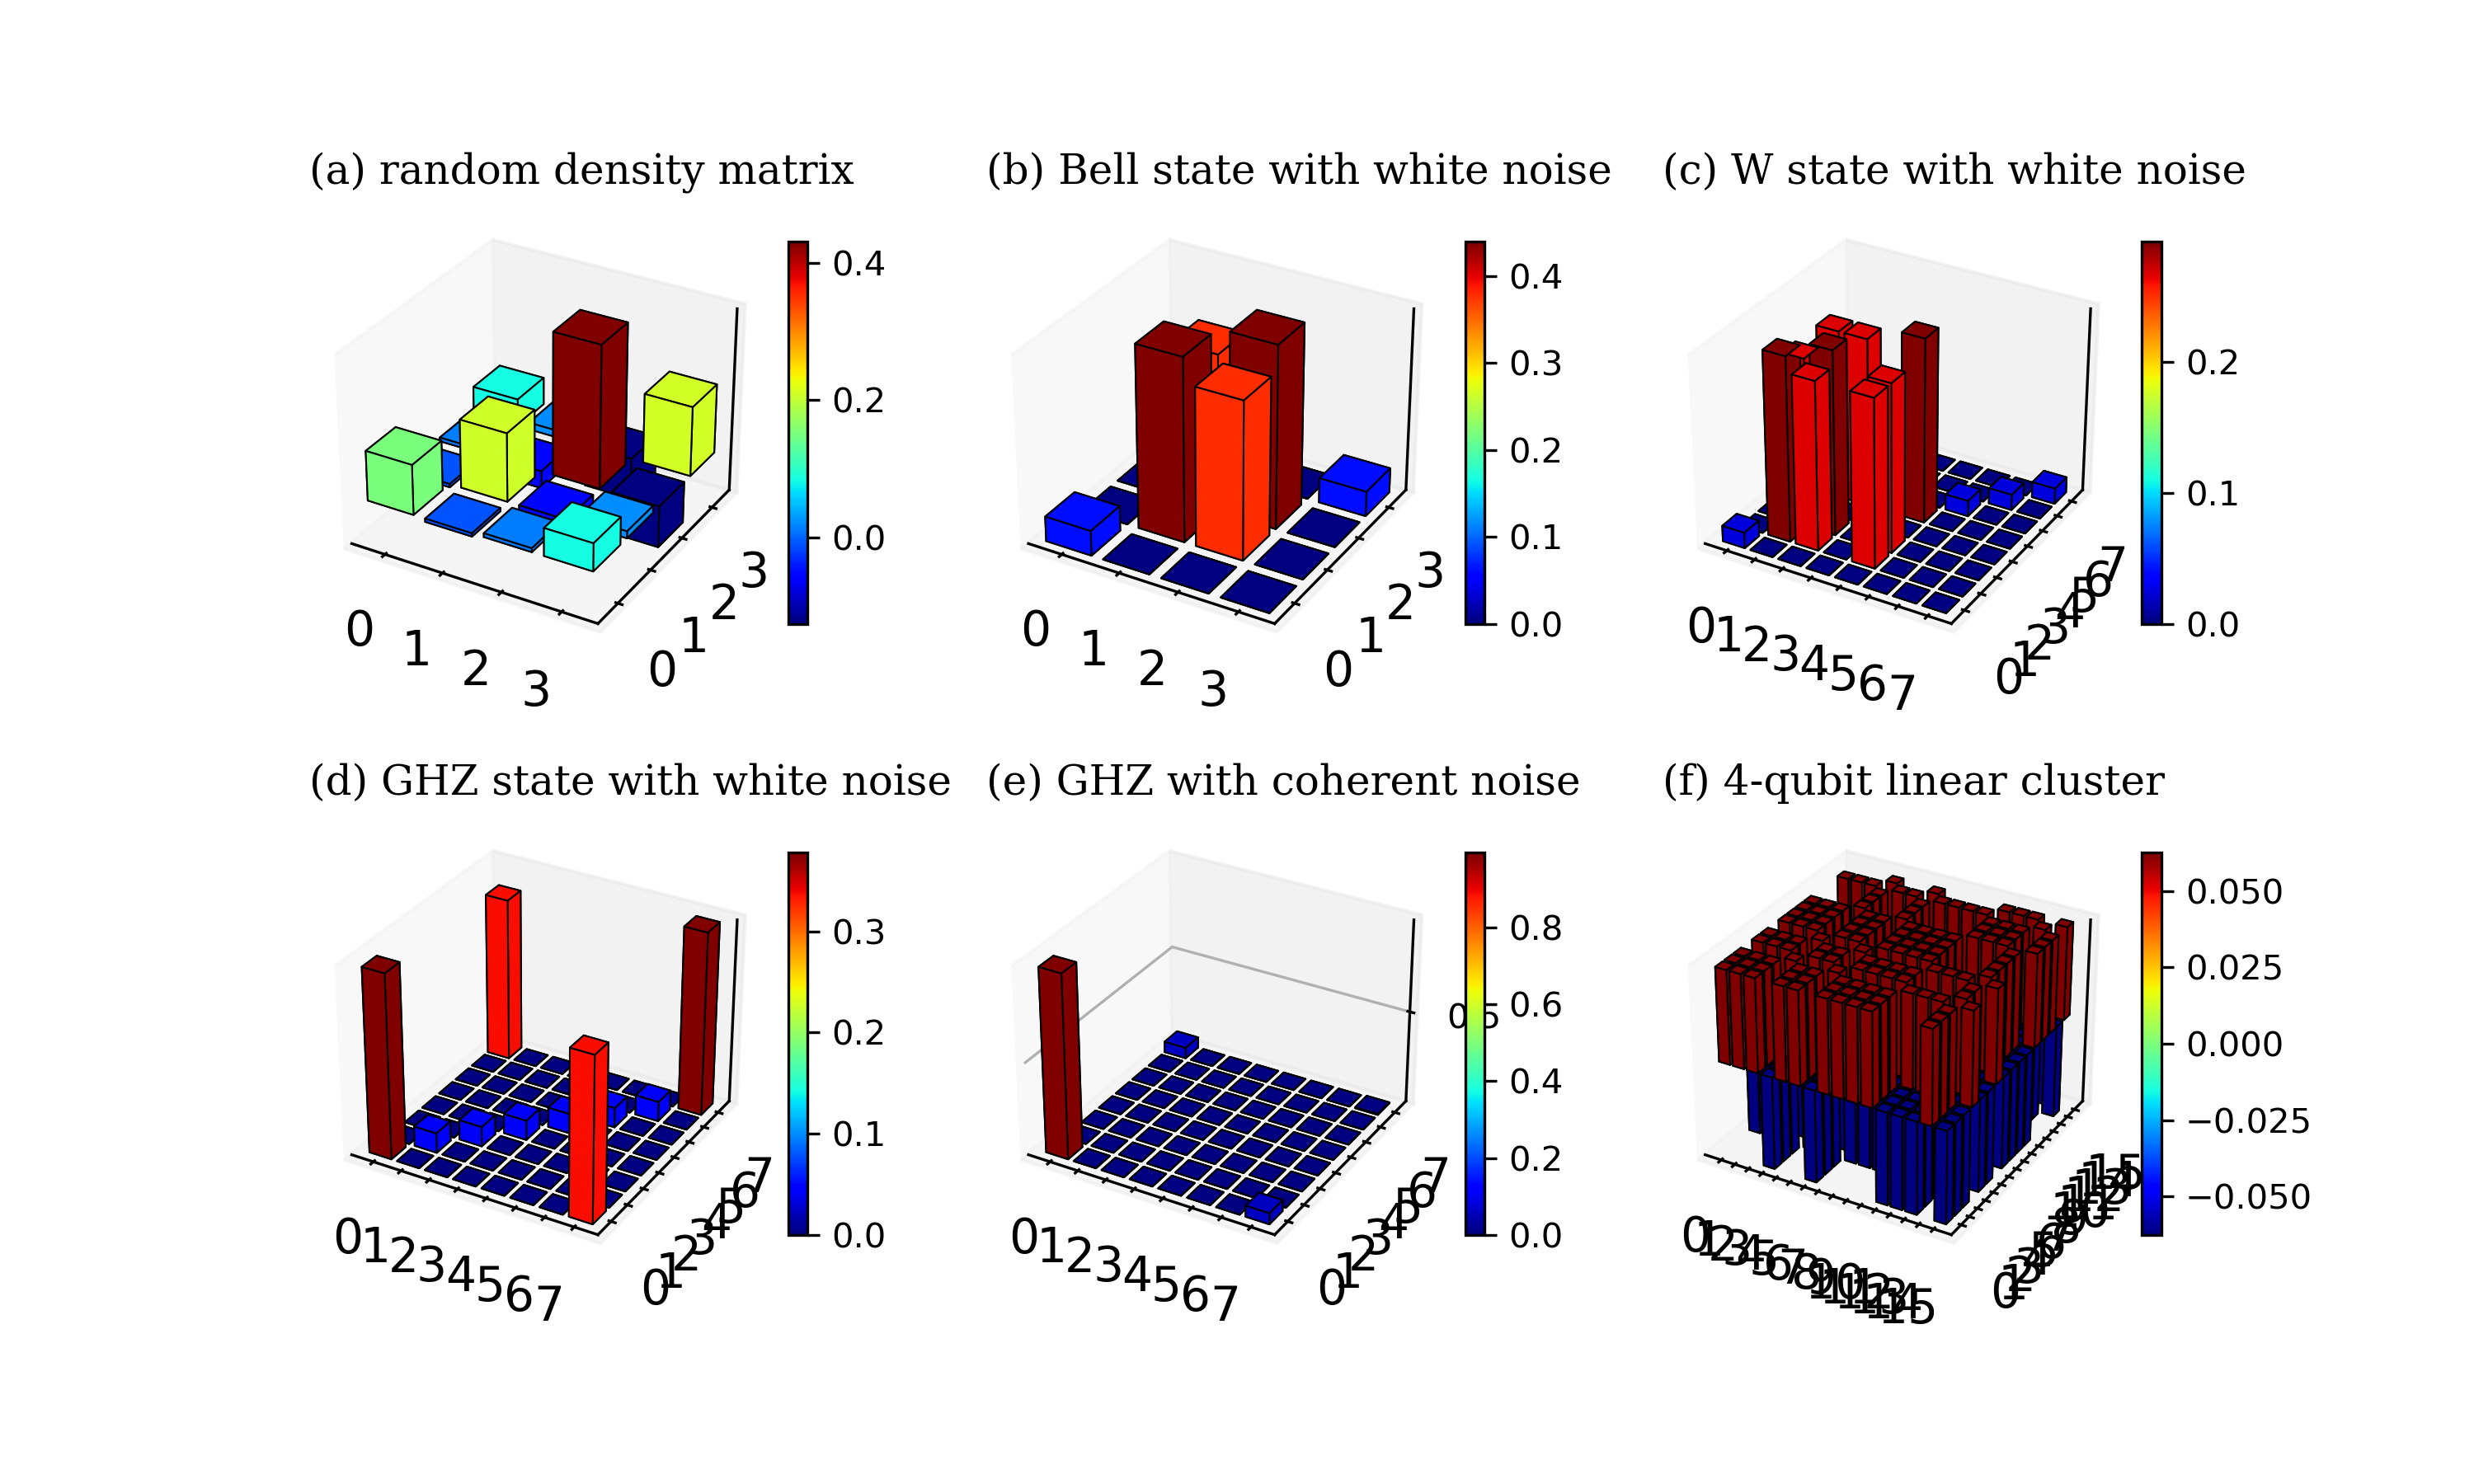
\includegraphics[width=.9\linewidth]{./Code/dataset_sample_3x2.png}
% 		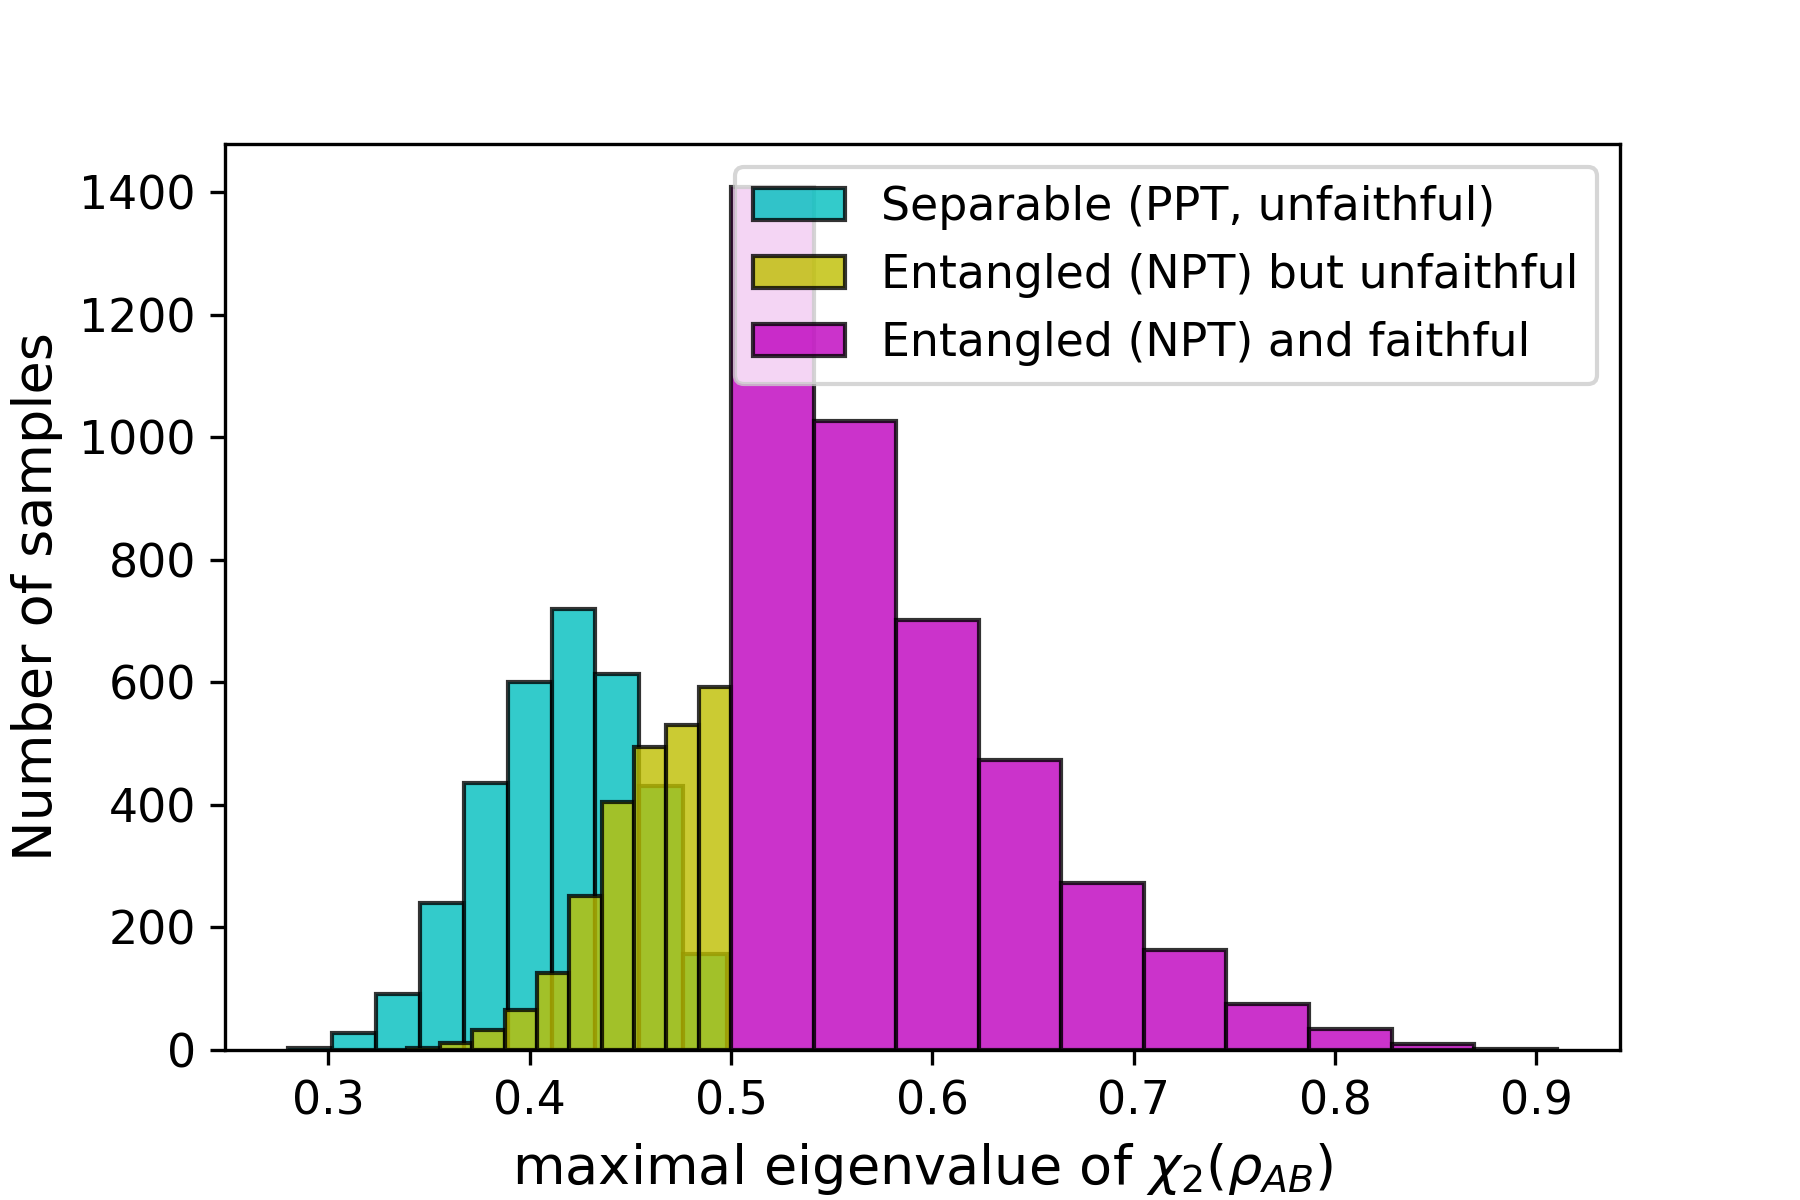
\includegraphics[width=.9\linewidth]{./Code/faithfulness_2_qubit.png}
	% \caption{PPT criterion (2-qubit random density matrix)}
	\caption{The real part of sampled density matrices: (a) a random 2-qubit state; (b) Bell state (singlet) with white noise; (c) 3-qubit W state with white noise; (d) 3-qubit GHZ state with white noise; (e) 3-qubit GHZ state with coherent noise; (f) a random 3-qubit bi-separable state. The 4-qubit states used in the numeric simulation \cref{fig:ml_compare} are the natural extensions of (c), (d), (e), (f).}
	\label{fig:sample_data}
\end{figure}
% \subsection{Classification accuracy and comparison}



% \subsubsection{Hyperparameters and settings}

% \begin{figure}[!ht]
% 	\centering
% 	\includegraphics[width=1\linewidth]{.pdf}
% 	\caption{accuracy VS number of features}
% \end{figure}
% The goal of recursively feature elimination (RFE) is to eliminate non-essential features by recursively considering smaller and smaller subsets of the original features using a greedy algorithm. Initially, RFE takes the SVM we trained and ranks the coefficients by their magnitudes, with the lowest one pruned away; then the model is trained again with the remaining features.

% \subsection{Robustness to noise}

% \begin{figure}[!ht]
% 	\centering
% 	% \includegraphics[width=1\linewidth]{.pdf}
% 	\caption{robustness: accuracy VS p noise }
% \end{figure}

% \subsubsection{Results, feature elimination}
% performance of different methods: 

For the machine learning part, we make use of scikit-learning Python package \cite{pedregosaScikitlearnMachineLearning2011} to train SVM with RBF kernel.
For training a 4-qubit SVM classifier with accuracy $0.999$, we generate $10^4$ states for each kind of states.
bi-separable states including $\dm_{1}\otimes \dm_{234}$ and $\dm_{12}\otimes \dm_{34}$.....
\cref{fig:conventional_witness} and \cref{fig:ml_compare} show that conventional fidelity witnesses cannot correctly classify when GHZ states with coherent noises $\theta=\pi/3,\phi>\pi/2$ (even mixed with white noise $p_\noise \in [0,0.1]$) and W states mixed with white noise $p_{\noise}>8/21$,
while the SVM classifier can classify them with hight accuracy.
\begin{figure}[!ht]
	% \begin{subfigure}{0.45\textwidth}
	\centering
		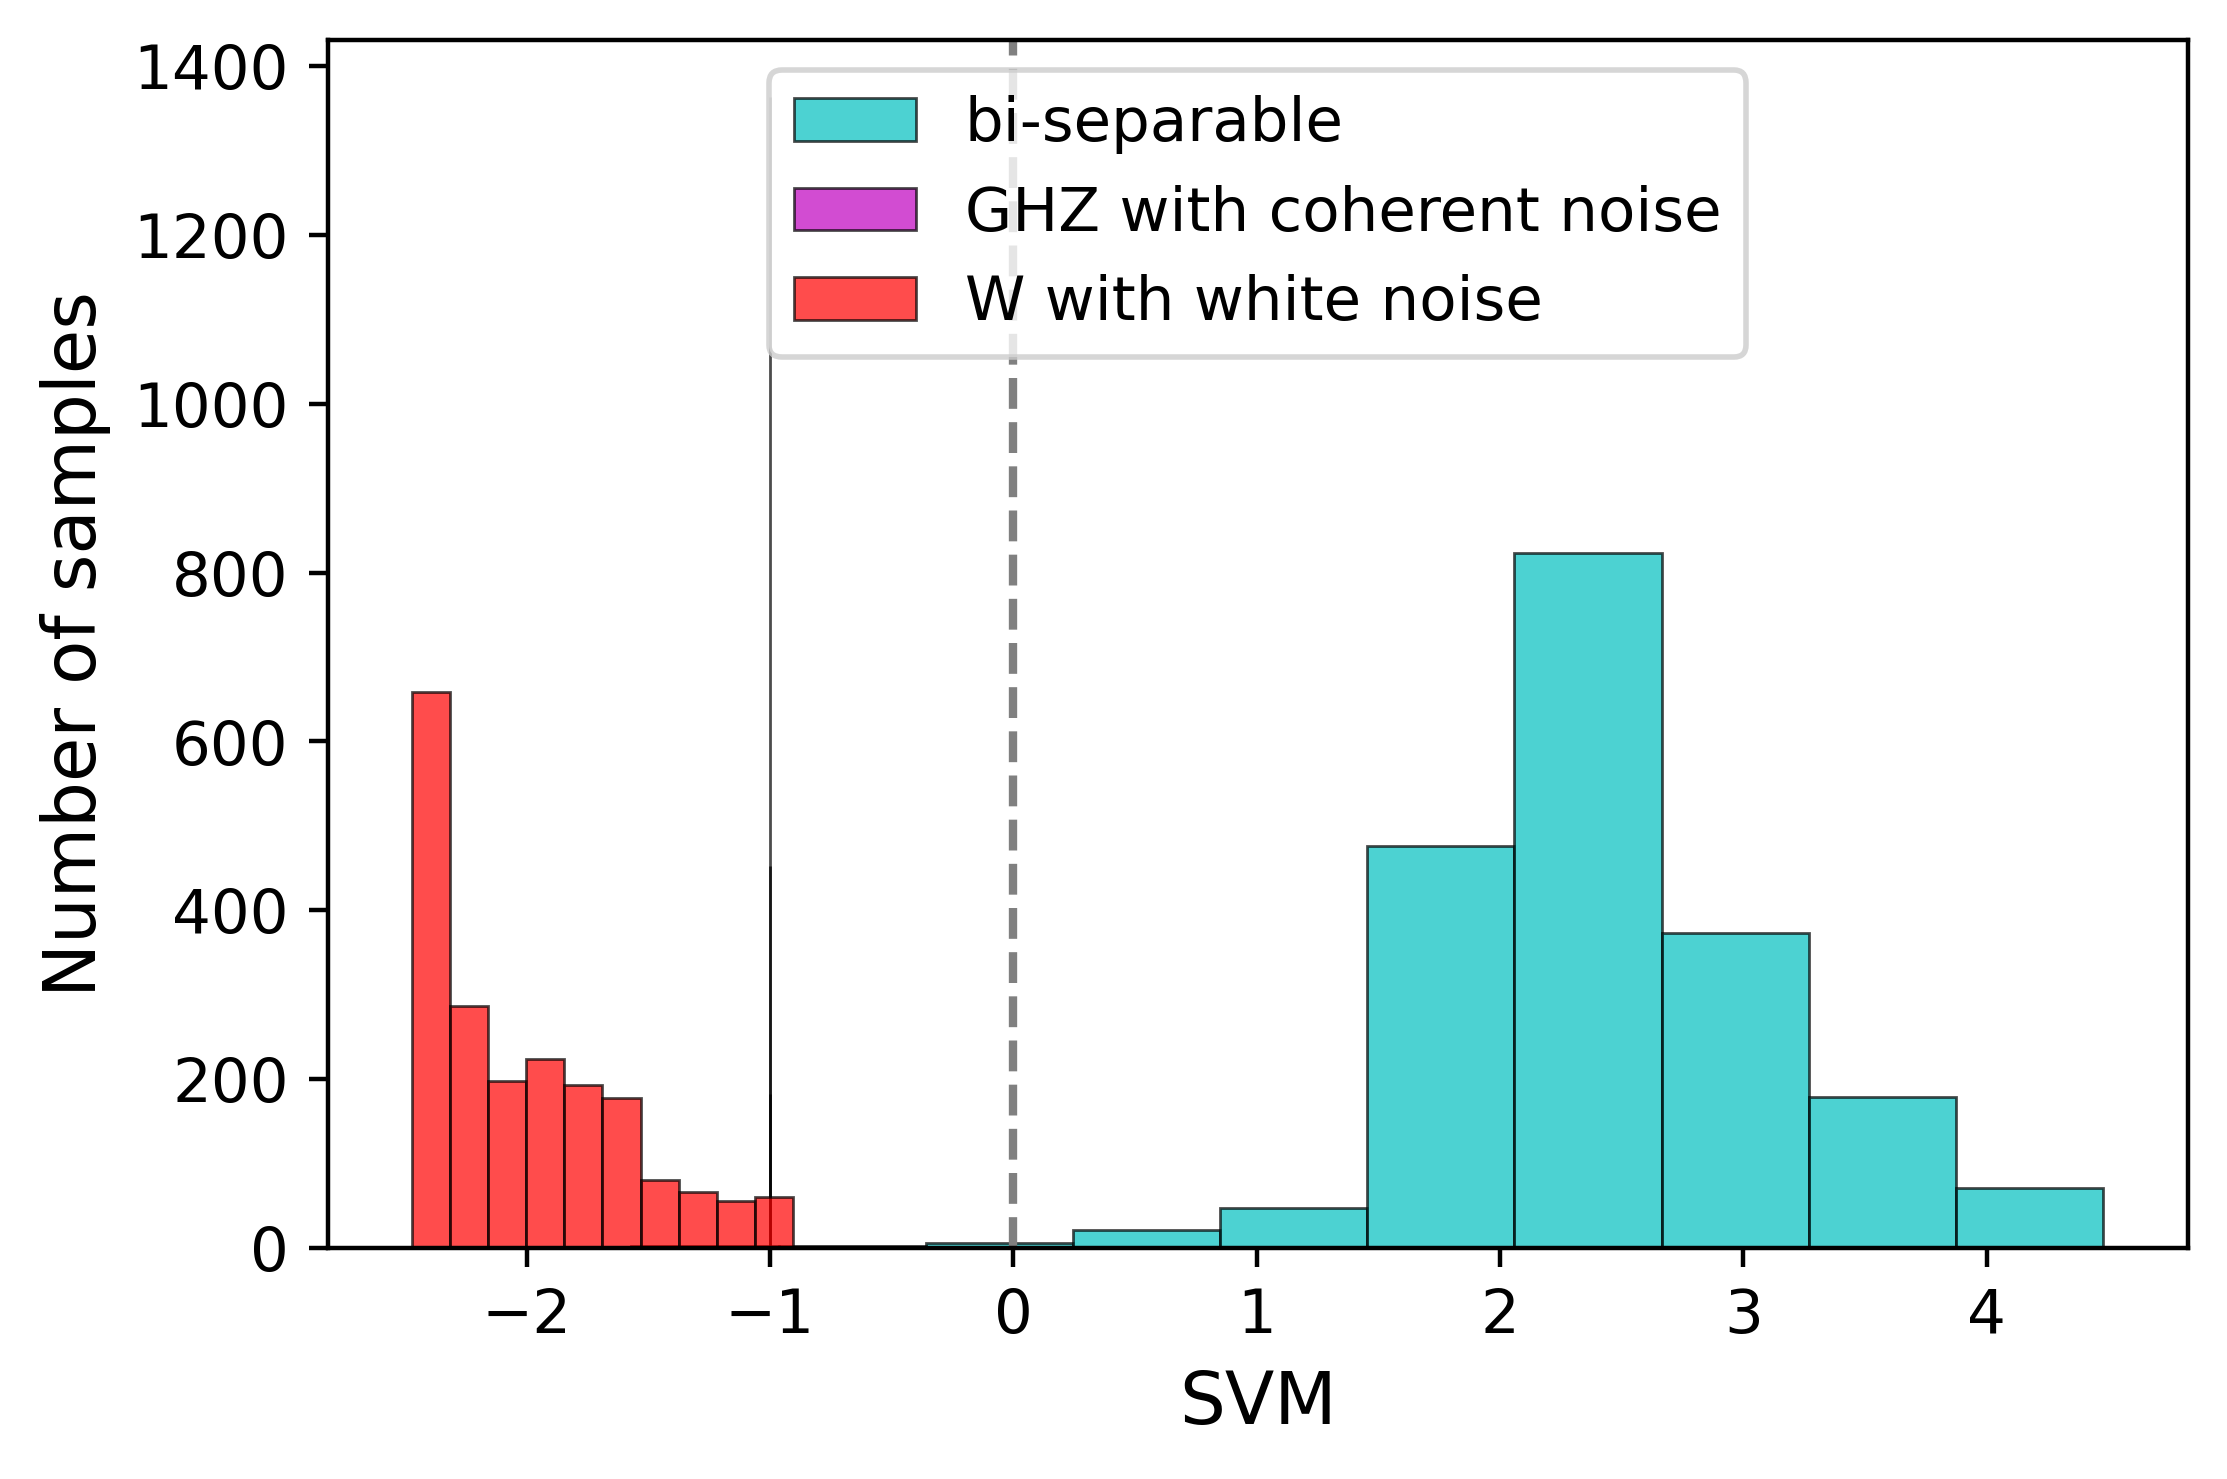
\includegraphics[width=.9\linewidth]{./Code/three_qubit_hist_ML.png}
		% 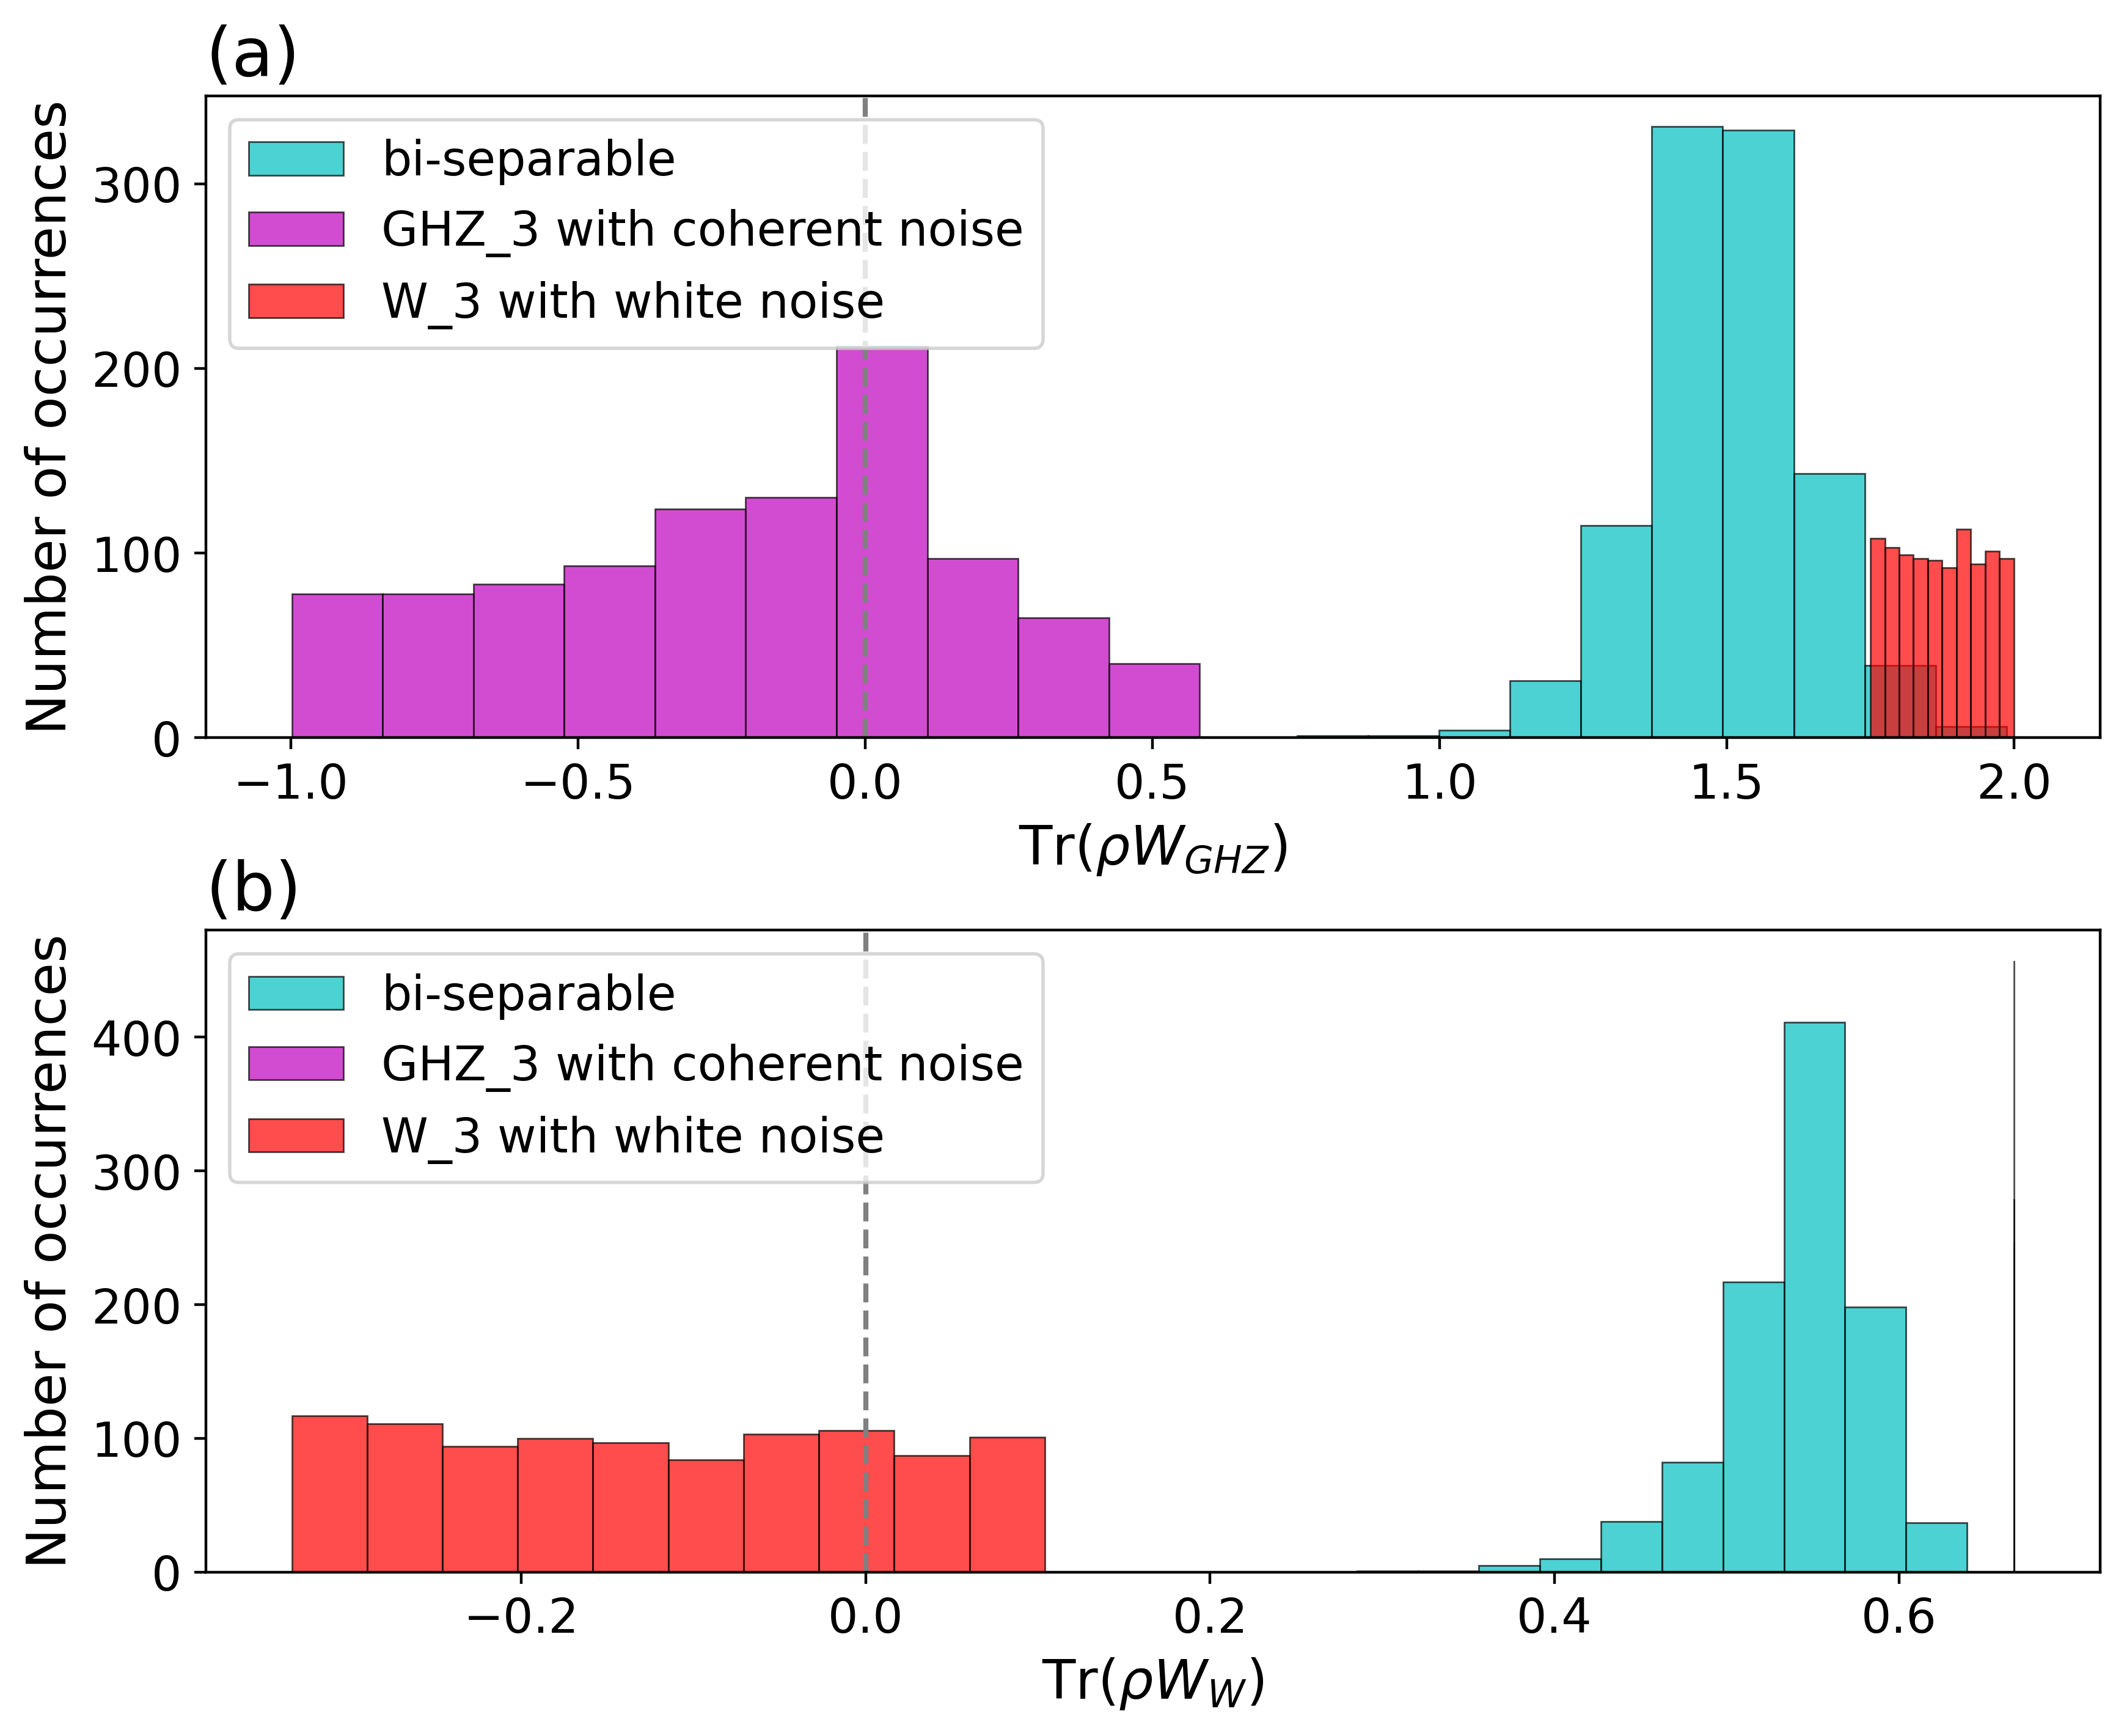
\includegraphics[width=.9\linewidth]{./Code/fidelity_witness_compare_2_long.png}
		% 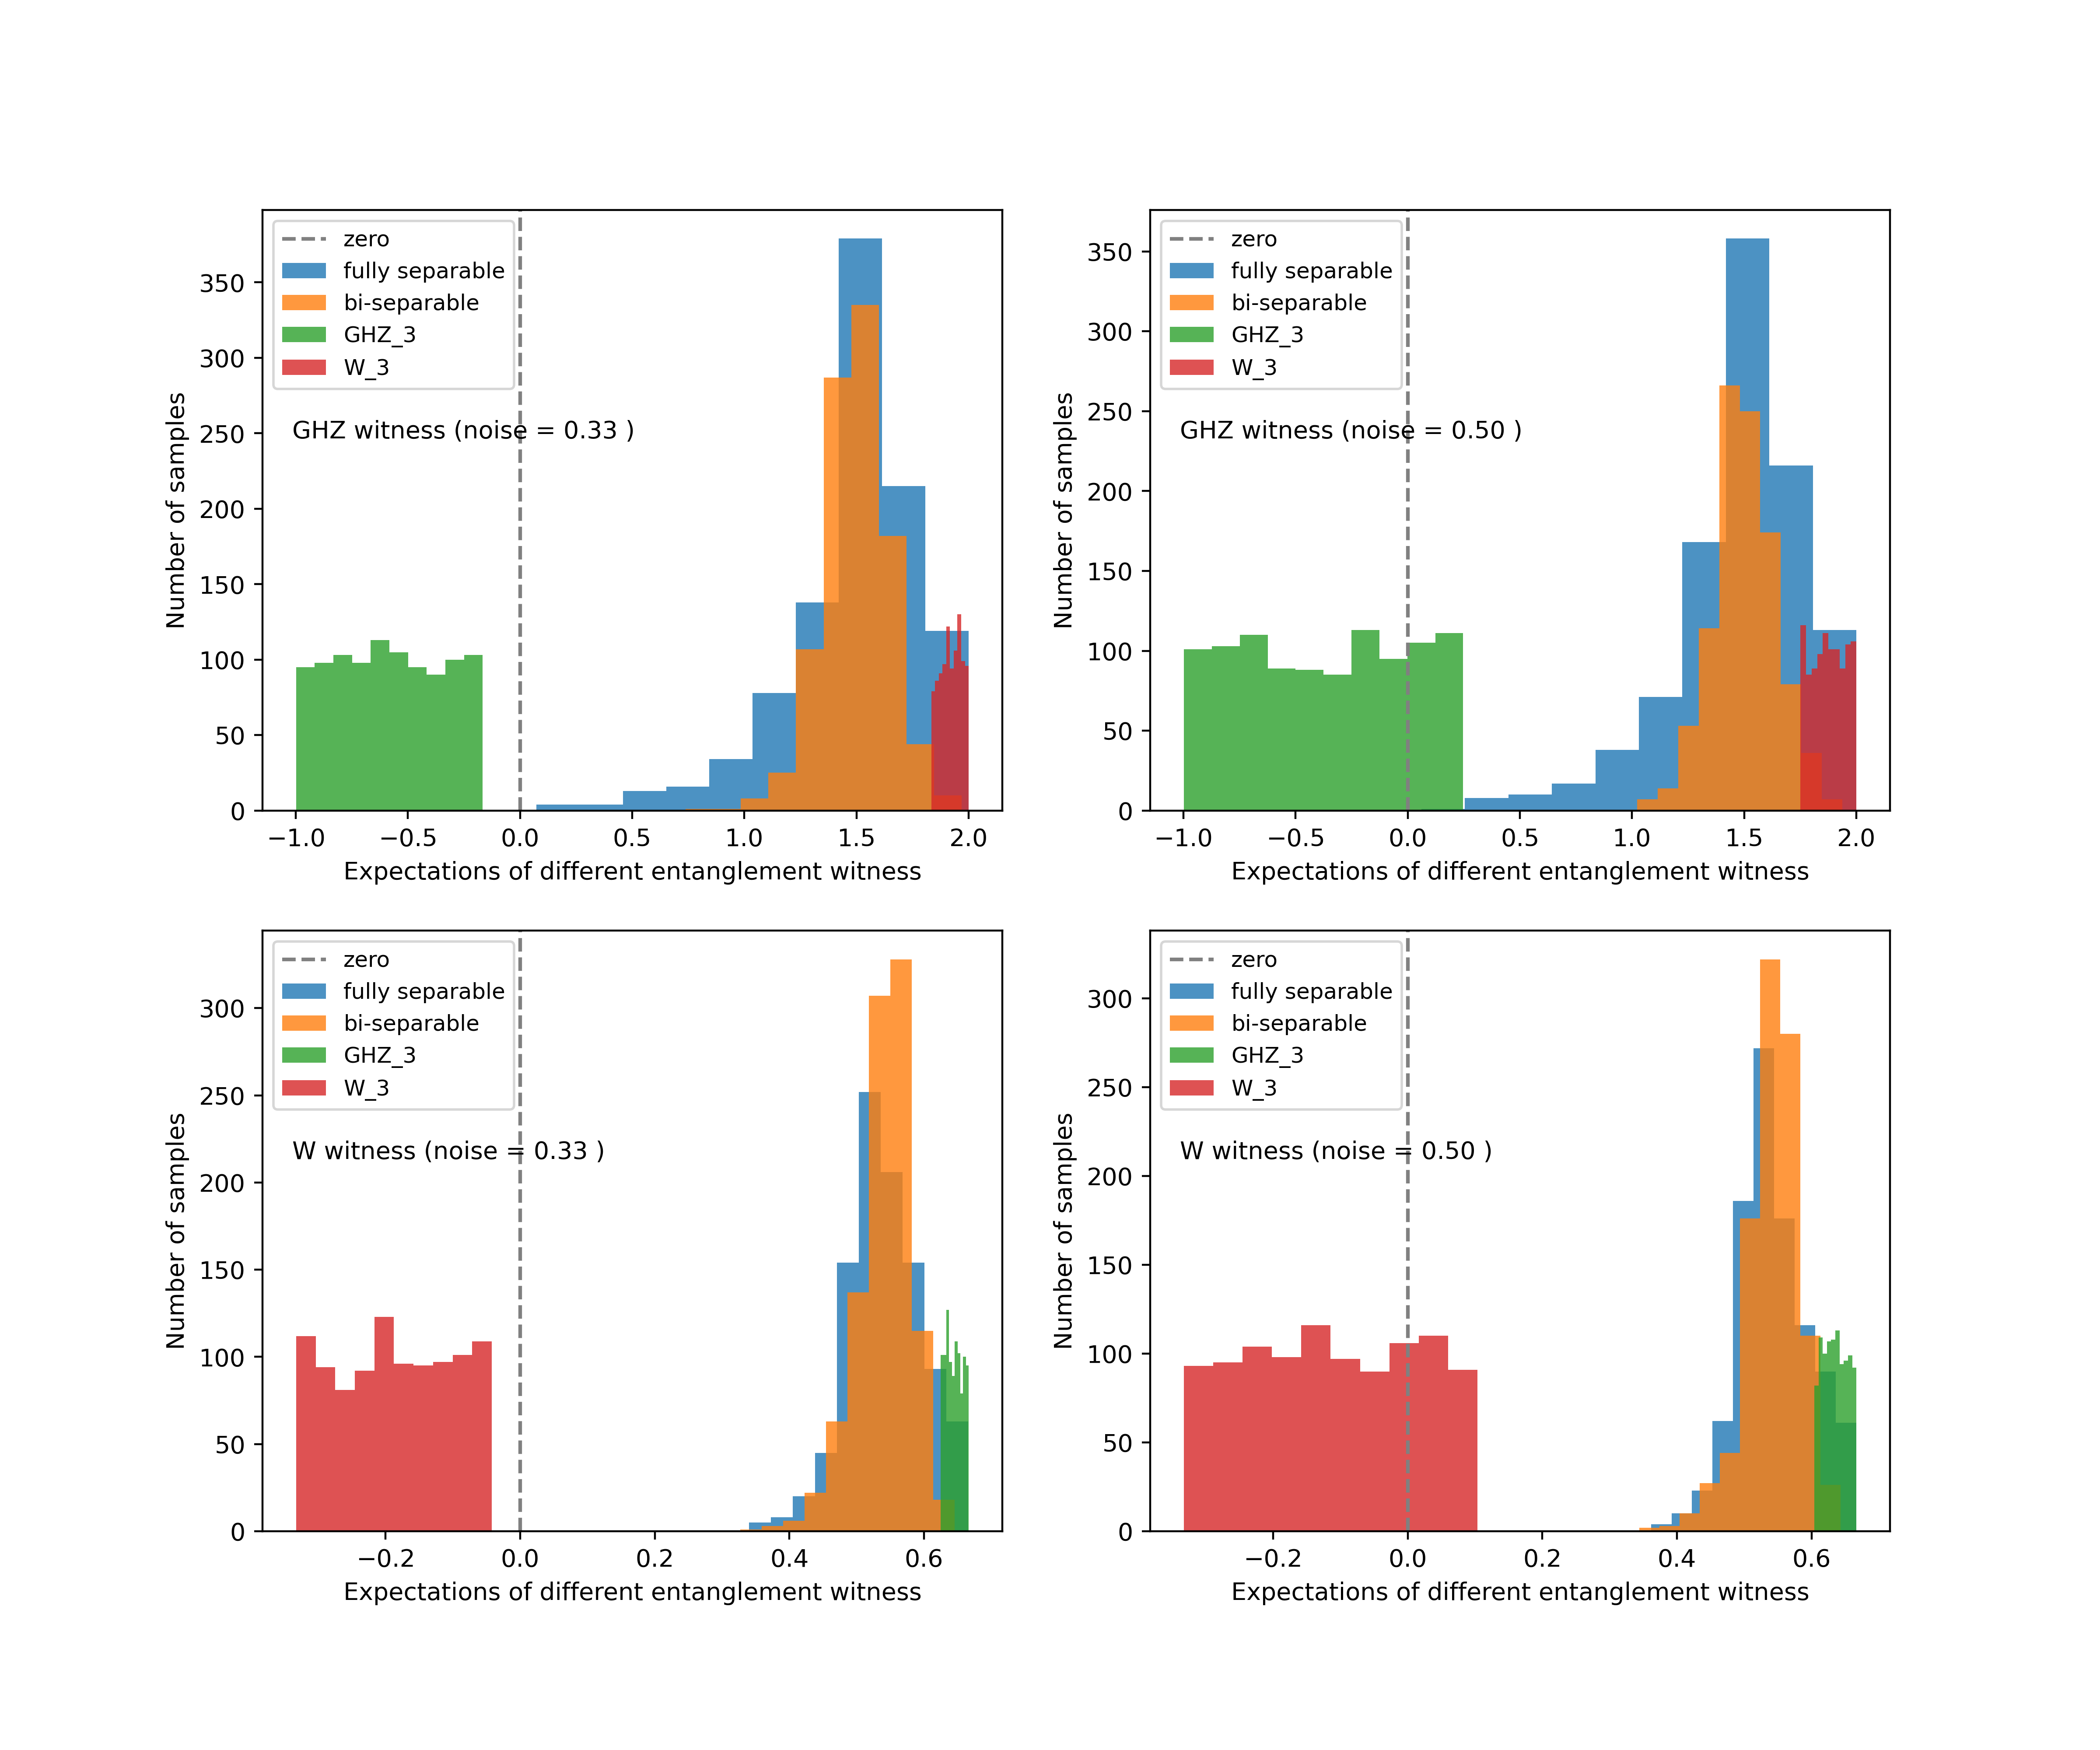
\includegraphics[width=.9\linewidth]{./Code/fidelity_witness_compare.png}
		% 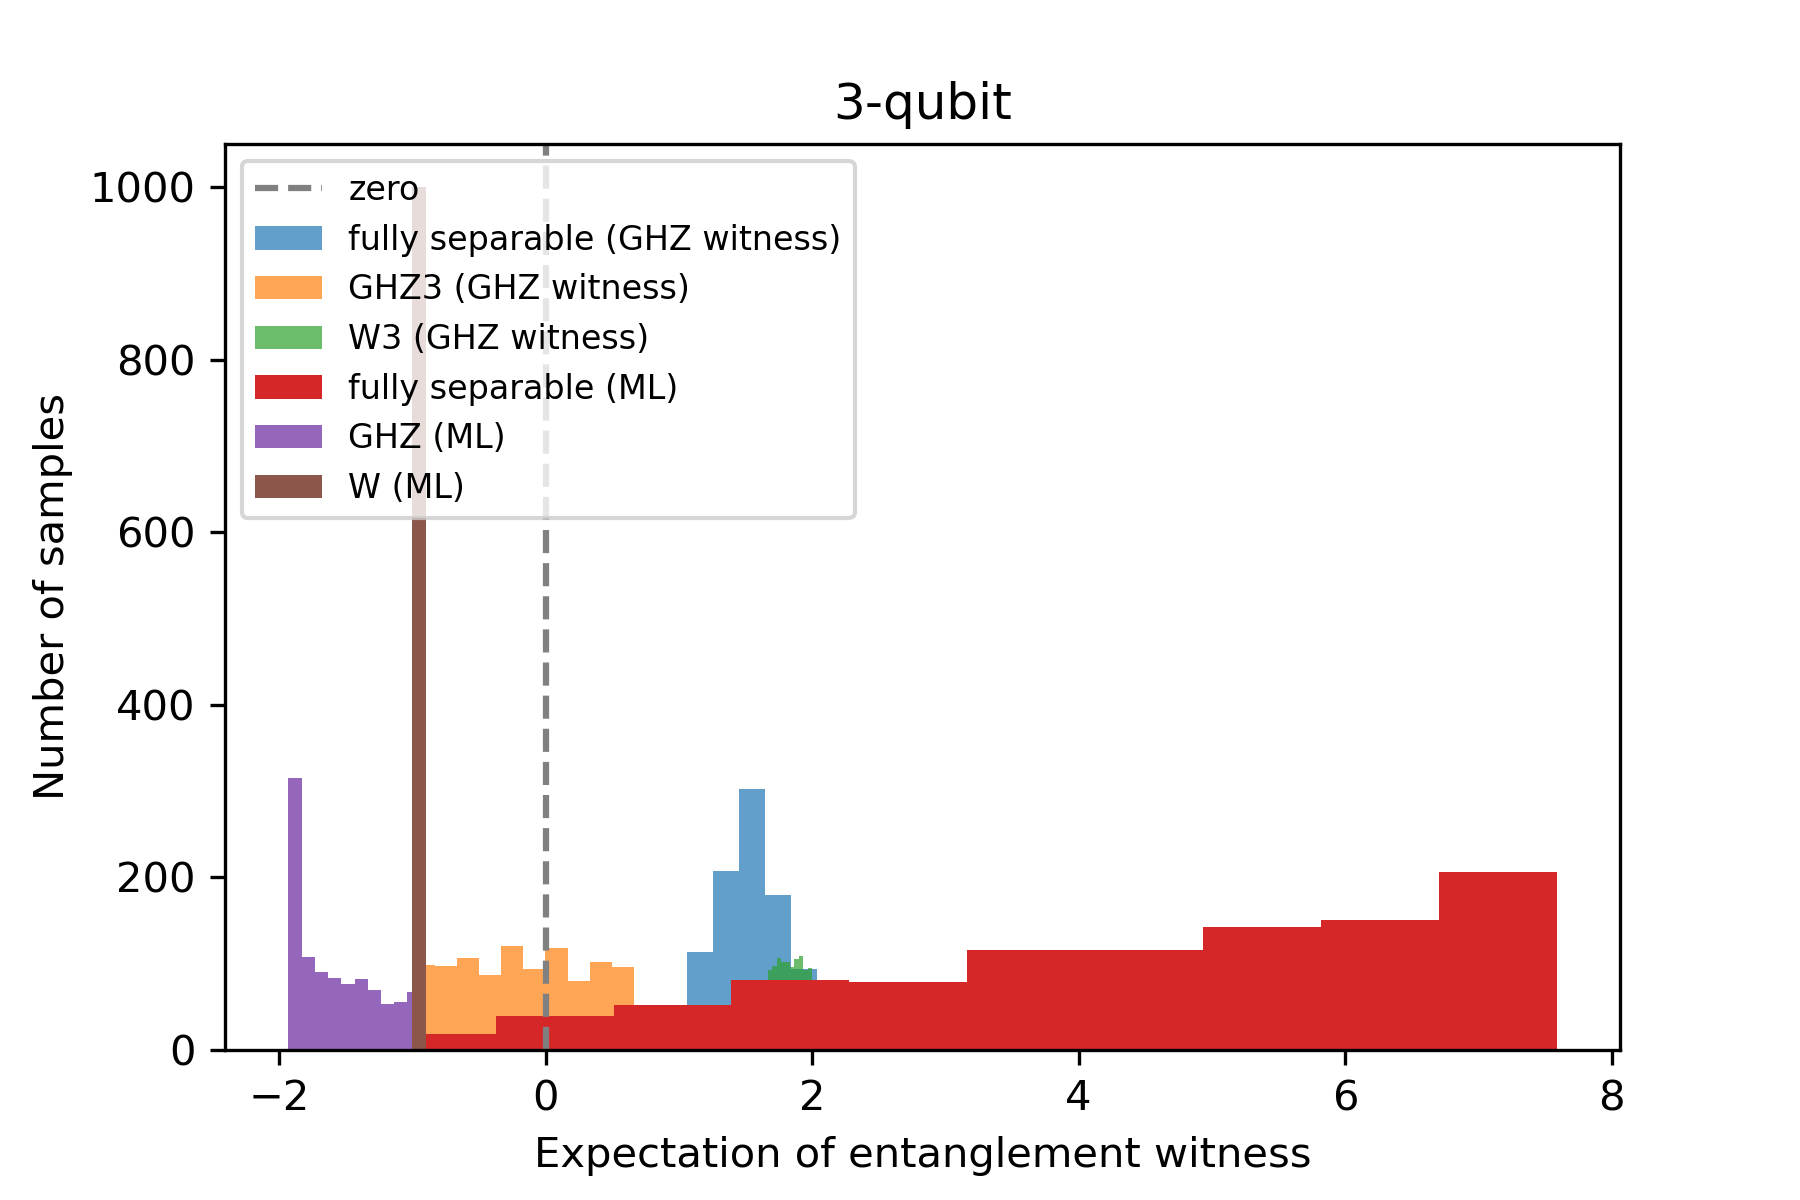
\includegraphics[width=.9\linewidth]{./notebook/three_qubit_hist.png}
		% \caption{ML witness, unfaithful}
	% \end{subfigure}
	% 	\caption{compare different methods: Bell inequality, witness, ML ansatz; different white noise limit, unfaithful state}
	\caption{The states beyond detection by fidelity witnesses (GHZ state with coherence noise $\theta\in[0,\pi/3], \phi\in[0,0.6\pi]$, and W state with large white noise $p_{\noise}\in[0,0.5]$) can be classified by the kernel SVM classifier with high accuracy.}
	\label{fig:ml_compare}
\end{figure}

One set of features found by the kernel SVM are 
$\vbx=\perm(\expval{XIIX},\expval{YIIZ},\expval{IIZZ},\expval{ZXII})$.
permutations $\perm:=[(1,2),(1,3),(1,4),(2,3),(2,4),(3,4)]$ and by symmetry of qubits of GHZ and W states....
% $\vbx=(\expval{ZZZ},\expval{XZX},\expval{ZZX},\expval{ZIZ},\expval{IZZ})$.
The error of estimating these features VS the size of shadow is shown in \cref{fig:shadow}.
\footnote{The open-source code for classical shadow with the code from \url{https://github.com/hsinyuan-huang/predicting-quantum-properties}}
(tradeoff between robustness and meaurement efficiency) 
The derandomized version performs better than randomized shadow and independent measurement.
The comparable size classical shadow has been implemented in photonic experiments  \cite{zhangExperimentalQuantumState2021}.
\begin{figure}[!ht]
	\centering
	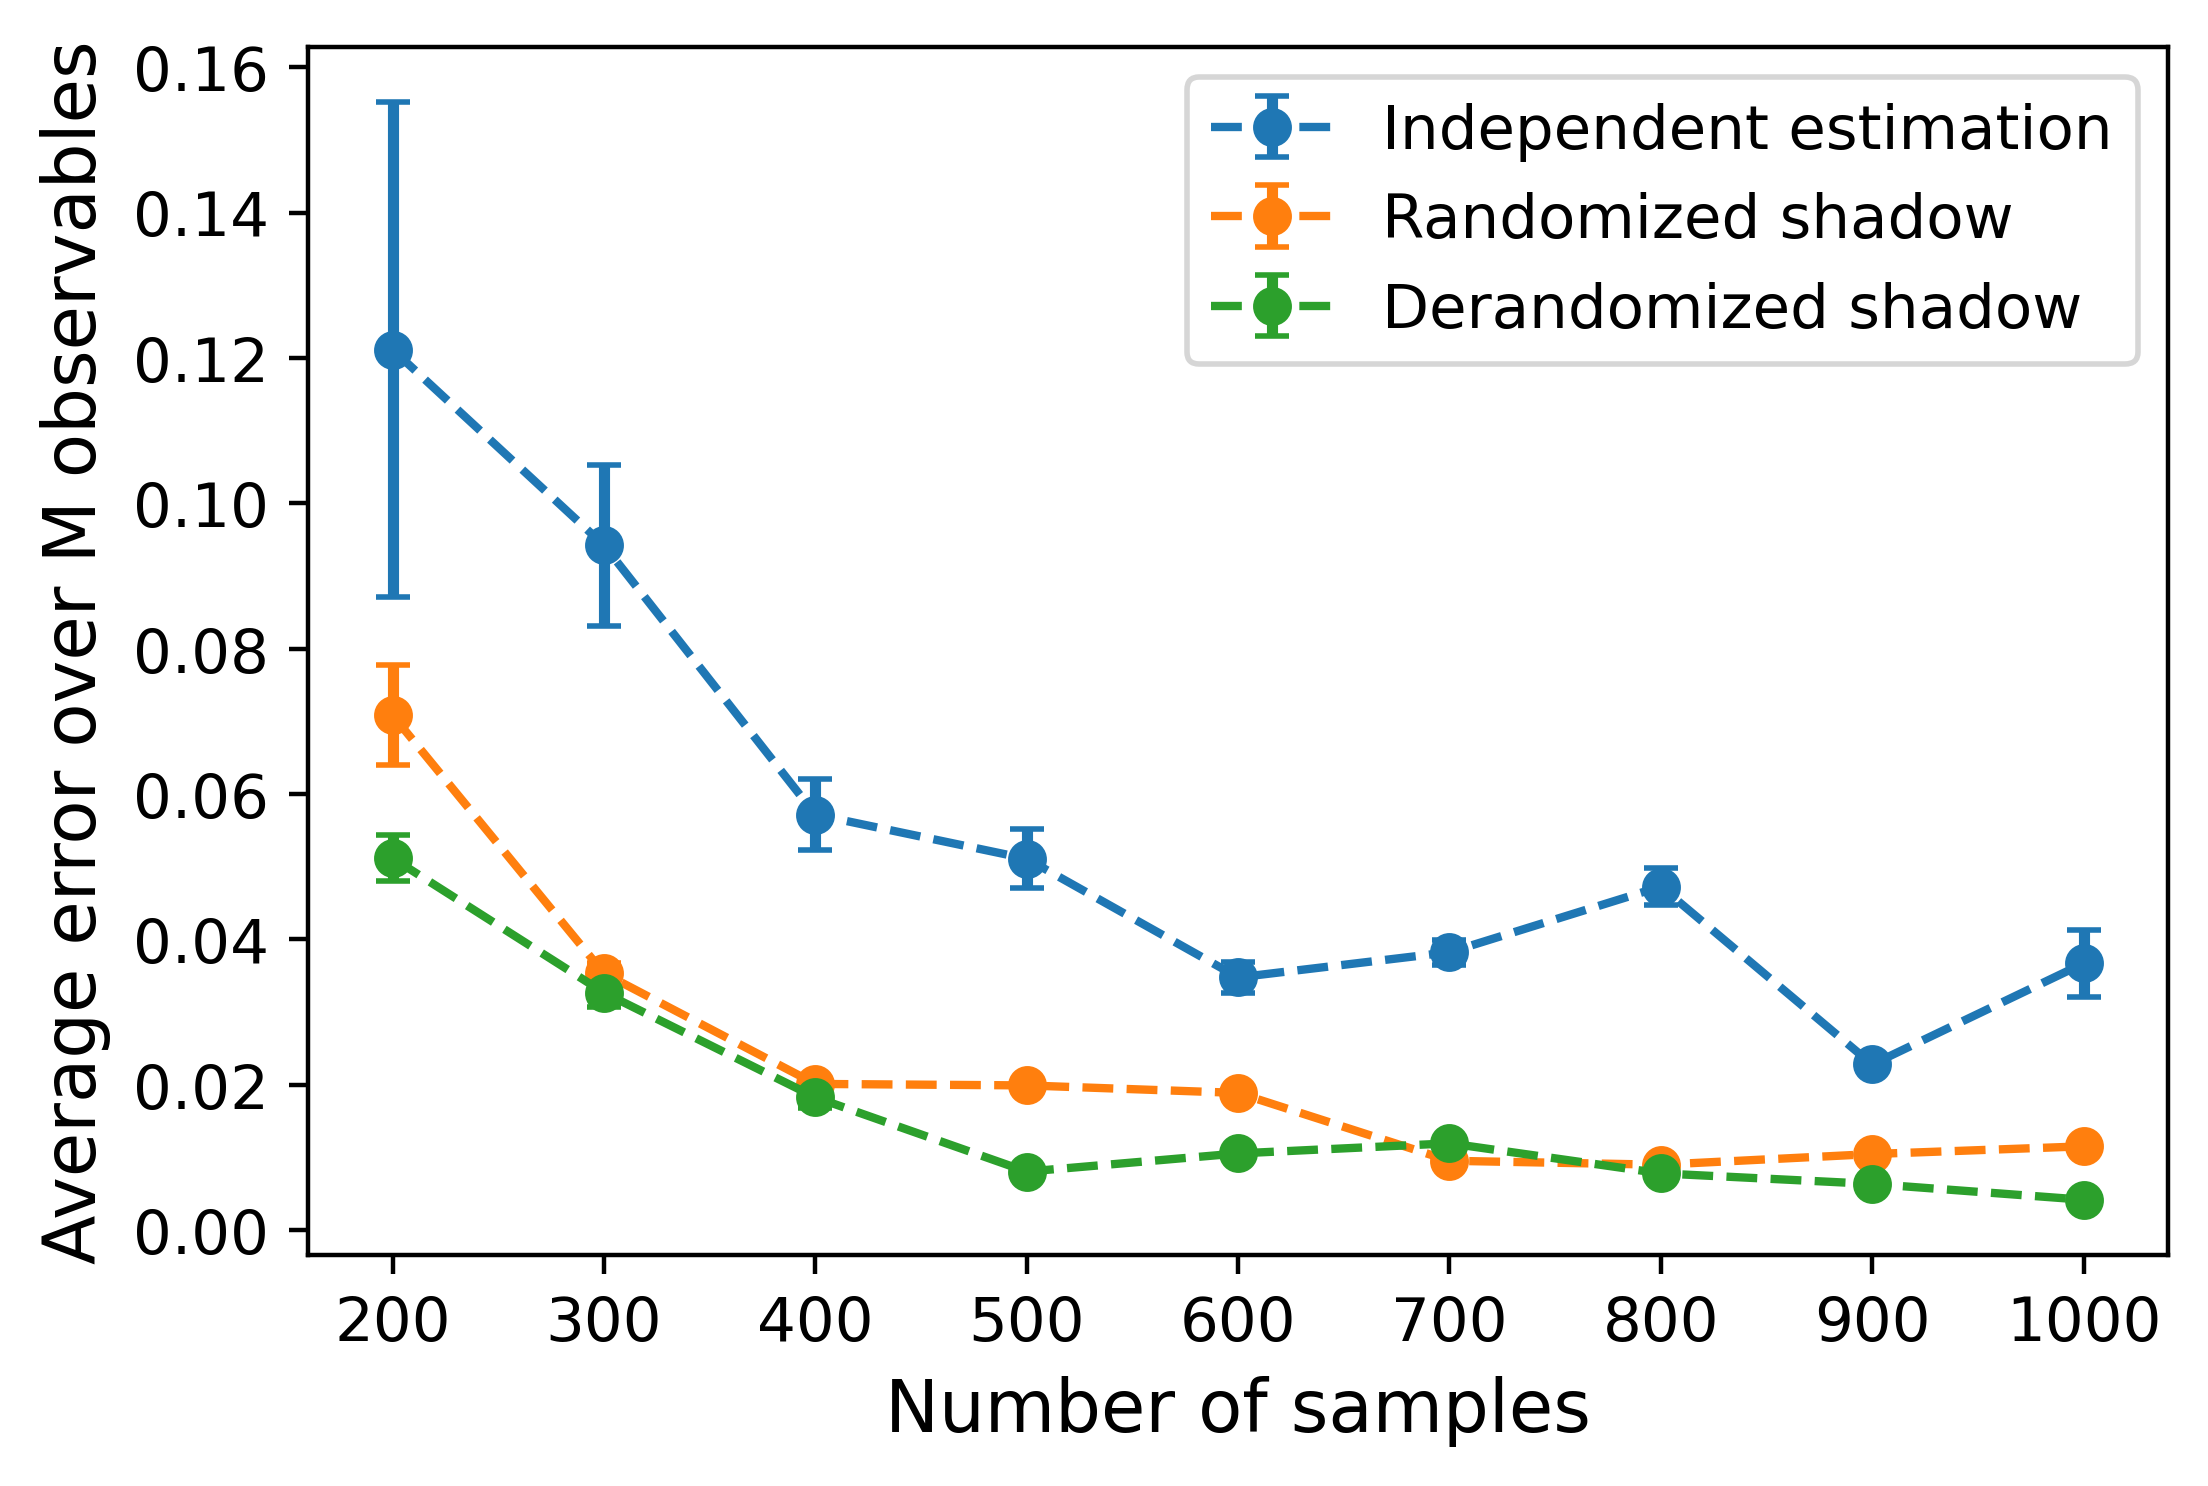
\includegraphics[width=.9\linewidth]{./Code/estimation_error_compare_methods.png}
	\caption{Average error of estimating expectation values of 30 2-local 4-qubit Pauli observables $\sum_i (o_i-\Tr(\ob_i\dm))^2/M$ by different estimation methods VS number of samples (the error bar indicates the standard deviation for each case). The blue line represents estimating each Pauli observables independently. The orange line is the estimation by the randomized classical shadow, while the green one is the derandomized version of classical shadow.}
	\label{fig:shadow}
\end{figure}

% We consider a set of different regularization parameters,...
% \begin{figure}[!ht]
% 	\centering
% 	% \includegraphics[width=1\linewidth]{.pdf}
% 	\caption{[TODO] accuracy VS dataset size, regularization parameters}
% \end{figure}


% \section{Experiments [TODO, hide]}\label{sec:experiments}
% \subsection{Experiments}
% Related experiments: photonic implementation with a few qubits (generation, verification) \cite{luEntanglementStructureEntanglement2018};
% fully entangled graph state (ring of 16 qubits) IBM by measuring negativity \cite{wang16qubitIBMUniversal2018};
% optical lattice (homogeneous, restricted measurement, detect GME, nonstabilizer) \cite{zhouSchemeCreateVerify2022};
% experiments of classical shadow and related comparison \cite{zhangExperimentalQuantumState2021};
% detect entanglement by estimating $p_3$-PPT with classical shadow \cite{elbenMixedstateEntanglementLocal2020}.
% Similar to the PPT condition, the $p_3$-PPT condition (without full tomography) applies to mixed states and is completely independent of the state in question \cite{elbenMixedstateEntanglementLocal2020}. 
% From this data set, the PT-moments $p_n=\Tr[(\dm_{AB}^{\T_A})^n]$ ($p_2=\Tr[\dm_{AB}^2]$ purity?) can be estimated without having to reconstruct the density matrix $\dm_{AB}$, and with a significantly smaller number of experimental runs $M$ than required for full quantum state tomography.
% c.f. \nameref{thm:multivariate_trace}, 
% \nameref{def:entanglement_spectroscopy}

% \section{Conclusion and discussion}\label{sec:conclusion}
% Related experiments: ....
In conclusion,
our protocol is flexible and sample-efficient in detecting entanglement around certain entangled state by training a kernel SVM classifier with a synthetic dataset.
We test our protocol for 4-qubit GHZ states with coherent noise and W states with large white noise.
We also show that the features for training such machine learned classifier can be estimated by a sample-efficient scheme....
% but no guarantee (need more research).
% The reason for choosing SVM as our machine learning technique is many-fold:
% (1) its clear geometric interpretation analoguous to entanglement witness;
% (2) the kernel SVM is powerful for classification and theoretically equivalent to Neural Network (nonlinear) in terms of neural tangent kernel \cite{jacotNeuralTangentKernel2020};
% % as they not only provide provable guarantees, but are also very flexible in the functions they can learn. 
% % For example, recent advancements in theoretical machine learning show that training neural networks with large hidden layers is equivalent to the neural tangent kernel \cite{jacotNeuralTangentKernel2020}.
% (3) the training of an SVM is convex: if a solution exists for the given target state and ansatz, the optimal SVM will be found;
% % (4) the SVM formalism allows for the programmatic elimination of features \cite{guyonGeneSelectionCancer2002}, i.e., reducing the cost of experimental measurements and copies (samples);
% % (5) only requires local (Pauli) measurements $\vbx:=\Tr(\dm\pob_{\sigma})$ even when the target state is a non-stabilizer state, such as W state, which normally need nonlocal measurements.
% % in exchange for a lower tolerance to white noise, in a manner similar 


There are also several potential directions for future research:
(1) It is of practical interest to find rigorous proof or perform numerical simulation for the dataset size and number of features (required for high training accuracy) scaling with the system size (more than 4 qubits);
(2) It is meaningful to test more kernels, such as graph kernel \cite{vishwanathanGraphKernels2010}, shadow kernel \cite{huangProvablyEfficientMachine2022}, and neural tangent kernel \cite{jacotNeuralTangentKernel2020}, for better performance of the kernel SVM.
% As a recent advancement in machine learning theory, the neural tangent kernel SVM is theoretically as powerful as Neural Network.
And quantum kernel methods \cite{schuldQuantumMachineLearning2019,schuldSupervisedQuantumMachine2021,liuRigorousRobustQuantum2021} also provide advantages over classical counterparts.
(3) 
% quantum machine learning for efficiently estimating all classical features allows for training a tomographic SVM classifier for wider range of states.
% \subsubsection{Estimate expectation by machine learning}
The task of estimating expectation values can also be achieved efficiently by both classical \cite{gaoEfficientRepresentationQuantum2017,torlaiManybodyQuantumState2018,zhuFlexibleLearningQuantum2022} and quantum machine learning \cite{huangPowerDataQuantum2021,huangProvablyEfficientMachine2022}.
% The quantum ML algorithm accesses the quantum channel $\mathcal{E}_\dm$ multiple times to obtain multiple copies of the underlying quantum state $\dm$. Each access to $\mathcal{E}_\dm$ allows us to obtain one copy of $\dm$. Then, the quantum ML algorithm performs a sequence of measurements on the copies of $\dm$ to accurately predict $\Tr(P_{\vbx} \dm ), \forall \vbx \in \qty{ I, X, Y, Z }^n$.
Huang et. al rigorously showed that, 
% for any quantum process $\mathcal{E}$, observables $\ob$, and distribution $\mathcal{D}$, and for any quantum ML model, one can always design a classical ML model achieving a similar average prediction error such that $N_C$ (number of experiments?) is larger than $N_Q$ by at worst a small polynomial factor.
% In contrast, 
for achieving accurate prediction on all $4^n-1$ Pauli observables 
% $\Tr(\dm\pob_{\sigma} ), \forall \sigma \in \qty{ I, X, Y, Z }^n$, 
the exponential quantum advantage over classical ML is possible
\cite{huangInformationtheoreticBoundsQuantum2021}.
Training a more powerful (universal) classifier with all Pauli observables as features might be interesting.
	% \footnote{
	% 	$\bigO(\log(M/\delta)\epsilon^{-4})$ copies of the unknown quantum state $\dm$.
	% 	($M=4^n$ implies linear copy for full tomography???)
	% }
	% \footnote{
	% 	% \cite{huangPowerDataQuantum2021}
	% 	the required amount of training data scales badly with $\epsilon$. This unfortunate scaling is not a shortcoming of the considered ML algorithm, but a necessary feature.
	% }
% (5) can we estimate concurrence... by quantum circuit;
% (6) quantum complexity for \nameref{prm:separability}


% \subsection*{Acknowledgements}
\begin{acknowledgments}
\end{acknowledgments}
% \thanks{The author thanks} 
% The author thanks
% TikZiT, QuTip

%\begin{appendices}
    %\chapter{}
%\end{appendices}

% %%%%%%%%%%%%%%%Reference%%%%%%%%%%%%%%%
% % \newpage
% % \printbibliography
\bibliographystyle{apsrev4-2}
%\bibliographystyle{alpha}
\bibliography{ref}

\onecolumngrid
\appendix

% \newpage
% \section{Definitions}\label{sec:definitions}

% \begin{definition}[Schmidt measure]\label{def:schmidt_measure}
% 	Consider the following bipartite pure state, written in Schmidt form:
% 	\begin{equation}
% 		\ket{\psi} = \sum_i^r \sqrt{\lambda_i} \ket{\phi_i^A}\otimes\ket{\phi_i^B}
% 		\label{eq:schmidt_decomposition}
% 	\end{equation}
% 	where $\qty{\ket{\phi_i^A}}$ is a basis for $\hilbertspace_A$ and $\qty{\ket{\phi_i^A}}$ for $\hilbertspace_B$.
% 	The strictly positive values $\sqrt{\lambda_i}$ in the Schmidt decomposition are its \emph{Schmidt coefficients}. 
% 	The number of Schmidt coefficients, counted with multiplicity, is called its \emph{Schmidt rank}, or Schmidt number. 
% 	Schmidt measure is minimum of $\log_2 r$ where $r$ is number of terms in an expansion of the state in product basis.
% 	(Schmidt rank ?? $\text{SR}^A(\psi)=\rank(\rho_{\psi}^A)$)
% \end{definition}
% \begin{remark}
% 	When a bipartite vector is written in the Schmidt basis, it is very easy to compute the partial trace of either subsystem	
% 	\begin{equation}
% 		\Tr_B(\op{\psi}) = \sum_i p_i \op{\phi_i^A}
% 	\end{equation}
% \end{remark}

% \subsubsection{Distance measures}\label{sec:distance_measure}
% \begin{definition}[fidelity]\label{def:fidelity}
% 	Given a pair of states (target $\dm$ and prepared $\dm'$), 
% 	Uhlmann fidelity $F(\dm,\dm') : = \Tr(\sqrt{\sqrt{\dm}\dm'\sqrt{\dm}})\equiv\norm{\sqrt{\dm}\sqrt{\dm'}}_1$, where $\sqrt{\dm}$ dentoes the positive semidefinite square root of the operator $\dm$. (infidelity $1-F(\dm,\dm')$)
% 	For any mixed state $\rho$ and pure state $\ket{\psi}$, $F(\dm,\op{\psi})=\sqrt{\mel{\psi}{\dm}{\psi}}\equiv \sqrt{\Tr(\dm\op{\psi})}$ which can be obtained by the Swap-test[?].
% 	linear fidelity or overlap $F(\dm,\dm'):=\tr(\dm\dm')$.
% 	% \begin{equation}
% 	% 	F(\ket{\psi},\ket{\psi'}) :=
% 	% \end{equation}
% 	% \begin{equation}
% 	% 	F(\rho,\rho') : = \Tr \sqrt{\sqrt{\rho}\rho'\sqrt{\rho}}
% 	% \end{equation}
% \end{definition}
% different distance measures \cite{badescuQuantumStateCertification2017}
% \begin{notation}[norm]\label{def:norm}
% 	Schatten p-norm $\norm{x}_p:= (\sum_i \abs{x_i}^p)^{1/p}$.
% 	Euclidean norm $l_2$ norm;
% 	Spectral (operator) norm $\norm{\vbx}_{\infty}$;
% 	Trace norm $\norm{A}_{\Tr}\equiv\norm{A}_{1}:=\Tr(\abs{A})\equiv\Tr(\sqrt{A^\dagger A})$, $\abs{A}:=\sqrt{A^\dagger A}$, $p=1$;
% 	% Frobenius norm $\norm{A}_{F}:=\sqrt{\Tr(A^\dagger A)}$, $p=2$;
% 	% Hilbert-Schmidt norm $\norm{A}_{HS}:=\sqrt{\sum_{i,j} A_{ij}^2 }=?\sum_{i\in I}\norm{Ae_i}_H^2$;
% 	% Hilbert-Schmidt inner product $\expval{A,B}_{\textup{HS}}:=\Tr(A^\dagger B)$,
% 	% Frobenius inner product $\expval{A,B}_{\textup{F}}:=\Tr(A^\dagger B)$?
% 	% (in finite-dimensionala Euclidean space, the HS norm is identical to the Frobenius norm)
% 	% Although the Hilbert-Schmidt distance is arguably not too meaningful, operationally, one can use Cauchy-Schwarz to relate it to the very natural trace distance. 
% 	% shadow norm ...
% \end{notation}
% \begin{definition}[distance]\label{def:distance}
% 	For mixed states, trace distance $d_{\tr}(\dm,\dm') : = \frac{1}{2} \norm{\dm-\dm'}_1$.
% 	For pure states, $d_{\tr}(\ket{\psi},\ket{\psi'}) : = \frac{1}{2}\norm{\op{\psi} -\op{\psi'}}_1 = \sqrt{1-\abs{\ip{\psi}{\psi'}}^2}$.
% 	% \begin{equation}
% 	% 	d_{tr}(\rho,\rho') : = \frac{1}{2} \norm{\rho-\rho'}_1
% 	% \end{equation}
% 	fidelity and trace distance are related by the inequalities
% 	$1-F\le D_{\tr}(\dm,\dm') \le \sqrt{1-F^2}$
% \end{definition}

% \section{Support Vector Machine}\label{sec:svm}

\end{document}